\documentclass[twoside]{book}

% Packages required by doxygen
\usepackage{fixltx2e}
\usepackage{calc}
\usepackage{doxygen}
\usepackage[export]{adjustbox} % also loads graphicx
\usepackage{graphicx}
\usepackage[utf8]{inputenc}
\usepackage{makeidx}
\usepackage{multicol}
\usepackage{multirow}
\PassOptionsToPackage{warn}{textcomp}
\usepackage{textcomp}
\usepackage[nointegrals]{wasysym}
\usepackage[table]{xcolor}

% Font selection
\usepackage[T1]{fontenc}
\usepackage[scaled=.90]{helvet}
\usepackage{courier}
\usepackage{amssymb}
\usepackage{sectsty}
\renewcommand{\familydefault}{\sfdefault}
\allsectionsfont{%
  \fontseries{bc}\selectfont%
  \color{darkgray}%
}
\renewcommand{\DoxyLabelFont}{%
  \fontseries{bc}\selectfont%
  \color{darkgray}%
}
\newcommand{\+}{\discretionary{\mbox{\scriptsize$\hookleftarrow$}}{}{}}

% Page & text layout
\usepackage{geometry}
\geometry{%
  a4paper,%
  top=2.5cm,%
  bottom=2.5cm,%
  left=2.5cm,%
  right=2.5cm%
}
\tolerance=750
\hfuzz=15pt
\hbadness=750
\setlength{\emergencystretch}{15pt}
\setlength{\parindent}{0cm}
\setlength{\parskip}{3ex plus 2ex minus 2ex}
\makeatletter
\renewcommand{\paragraph}{%
  \@startsection{paragraph}{4}{0ex}{-1.0ex}{1.0ex}{%
    \normalfont\normalsize\bfseries\SS@parafont%
  }%
}
\renewcommand{\subparagraph}{%
  \@startsection{subparagraph}{5}{0ex}{-1.0ex}{1.0ex}{%
    \normalfont\normalsize\bfseries\SS@subparafont%
  }%
}
\makeatother

% Headers & footers
\usepackage{fancyhdr}
\pagestyle{fancyplain}
\fancyhead[LE]{\fancyplain{}{\bfseries\thepage}}
\fancyhead[CE]{\fancyplain{}{}}
\fancyhead[RE]{\fancyplain{}{\bfseries\leftmark}}
\fancyhead[LO]{\fancyplain{}{\bfseries\rightmark}}
\fancyhead[CO]{\fancyplain{}{}}
\fancyhead[RO]{\fancyplain{}{\bfseries\thepage}}
\fancyfoot[LE]{\fancyplain{}{}}
\fancyfoot[CE]{\fancyplain{}{}}
\fancyfoot[RE]{\fancyplain{}{\bfseries\scriptsize Generated by Doxygen }}
\fancyfoot[LO]{\fancyplain{}{\bfseries\scriptsize Generated by Doxygen }}
\fancyfoot[CO]{\fancyplain{}{}}
\fancyfoot[RO]{\fancyplain{}{}}
\renewcommand{\footrulewidth}{0.4pt}
\renewcommand{\chaptermark}[1]{%
  \markboth{#1}{}%
}
\renewcommand{\sectionmark}[1]{%
  \markright{\thesection\ #1}%
}

% Indices & bibliography
\usepackage{natbib}
\usepackage[titles]{tocloft}
\setcounter{tocdepth}{3}
\setcounter{secnumdepth}{5}
\makeindex

% Hyperlinks (required, but should be loaded last)
\usepackage{ifpdf}
\ifpdf
  \usepackage[pdftex,pagebackref=true]{hyperref}
\else
  \usepackage[ps2pdf,pagebackref=true]{hyperref}
\fi
\hypersetup{%
  colorlinks=true,%
  linkcolor=blue,%
  citecolor=blue,%
  unicode%
}

% Custom commands
\newcommand{\clearemptydoublepage}{%
  \newpage{\pagestyle{empty}\cleardoublepage}%
}

\usepackage{caption}
\captionsetup{labelsep=space,justification=centering,font={bf},singlelinecheck=off,skip=4pt,position=top}

%===== C O N T E N T S =====

\begin{document}

% Titlepage & ToC
\hypersetup{pageanchor=false,
             bookmarksnumbered=true,
             pdfencoding=unicode
            }
\pagenumbering{alph}
\begin{titlepage}
\vspace*{7cm}
\begin{center}%
{\Large spmv }\\
\vspace*{1cm}
{\large Generated by Doxygen 1.8.13}\\
\end{center}
\end{titlepage}
\clearemptydoublepage
\pagenumbering{roman}
\tableofcontents
\clearemptydoublepage
\pagenumbering{arabic}
\hypersetup{pageanchor=true}

%--- Begin generated contents ---
\chapter{Build}
\label{md__home_tau_public_html_lecture_parallel_distributed_2018_parallel-distributed-handson_03spmv_README}
\Hypertarget{md__home_tau_public_html_lecture_parallel_distributed_2018_parallel-distributed-handson_03spmv_README}

\begin{DoxyCode}
$ make
g++  -Wall -Wextra -O3 -fopenmp   -c -o spmv.o spmv.cc
g++ -o spmv spmv.o  -Wall -Wextra -O3 -fopenmp 
\end{DoxyCode}


do this on the login node.

\section*{Run }

Example\+:


\begin{DoxyCode}
$ srun -p big ./spmv 
A : 100000 x 100000, 100000000 non-zeros 800000000 bytes for non-zeros
repeat : 5 times
1000000000 flops
repeat\_spmv : warm up + error check
repeat\_spmv : start
2002500000 flops in 6.514223060e+00 sec (3.074042724e-01 GFLOPS)
lambda = 5.006385423e+02
\end{DoxyCode}


srun should be used to run any executable on a compute node.

But for a very small/short run for the purpose of quick correctness check, you can directly run it on the login node.


\begin{DoxyCode}
$ ./spmv 
A : 100000 x 100000, 100000000 non-zeros 800000000 bytes for non-zeros
repeat : 5 times
1000000000 flops
repeat\_spmv : warm up + error check
repeat\_spmv : start
2002500000 flops in 6.514223060e+00 sec (3.074042724e-01 GFLOPS)
lambda = 5.006385423e+02
\end{DoxyCode}


\section*{help }

Just run


\begin{DoxyCode}
$ ./spmv -h
usage:

./spmv [options ...]

options:
  --help        show this help
  --M N         set the number of rows to N [100000]
  --N N         set the number of colums to N [0]
  --nnz N       set the number of non-zero elements to N [0]
  --repeat N    repeat N times [5]
  --format F    set sparse matrix format to F [coo]
  --algo A      set algorithm to A [serial]
  --seed S      set random seed to S [4567890123]
\end{DoxyCode}


\section*{Learn how it works }

Compile it with -\/\+O0 -\/g options and run it with small parameters inside a debugger.


\begin{DoxyCode}
$ ... modify Makefile and set -O0 and -g to cflags ...

$ make -B
g++  -Wall -Wextra -O0 -g -fopenmp   -c -o spmv.o spmv.cc
g++ -o spmv spmv.o  -Wall -Wextra -O0 -g -fopenmp

$ gdb ./spmv

   ...
Reading symbols from ./spmv...done.

(gdb) b main
Breakpoint 1 at 0x402dc8: file spmv.cc, line 790.

(gdb) run --M 10
Starting program: /home/tau/parallel-distributed-handson/00spmv/spmv --M 10
[Thread debugging using libthread\_db enabled]
Using host libthread\_db library "/lib/x86\_64-linux-gnu/libthread\_db.so.1".

Breakpoint 1, main (argc=3, argv=0x7fffffffe828) at spmv.cc:790
790     int main(int argc, char ** argv) \{
\end{DoxyCode}


If you use Emacs, it is much better to use it from within Emacs.


\begin{DoxyCode}
M-x gud-gdb
\end{DoxyCode}


and continue as before.

\section*{How to modify the file }
\chapter{Class Index}
\section{Class List}
Here are the classes, structs, unions and interfaces with brief descriptions\+:\begin{DoxyCompactList}
\item\contentsline{section}{\hyperlink{structcmdline__options__t}{cmdline\+\_\+options\+\_\+t} \\*Command line option }{\pageref{structcmdline__options__t}}{}
\item\contentsline{section}{\hyperlink{structcoo__elem__t}{coo\+\_\+elem\+\_\+t} \\*Element of coordinate list (i, j, a) }{\pageref{structcoo__elem__t}}{}
\item\contentsline{section}{\hyperlink{structcoo__t}{coo\+\_\+t} \\*Sparse matrix in coodinate list format }{\pageref{structcoo__t}}{}
\item\contentsline{section}{\hyperlink{structcsr__elem__t}{csr\+\_\+elem\+\_\+t} \\*Element of compressed sparse row }{\pageref{structcsr__elem__t}}{}
\item\contentsline{section}{\hyperlink{structcsr__t}{csr\+\_\+t} \\*Sparse matrix in compressed row format }{\pageref{structcsr__t}}{}
\item\contentsline{section}{\hyperlink{structidx__pair__t}{idx\+\_\+pair\+\_\+t} \\*Pair of two indices (i and j) }{\pageref{structidx__pair__t}}{}
\item\contentsline{section}{\hyperlink{structimage__t}{image\+\_\+t} \\*Data structure through which to convert a matrix into a gnuplot file }{\pageref{structimage__t}}{}
\item\contentsline{section}{\hyperlink{structsparse__format__table__entry__t}{sparse\+\_\+format\+\_\+table\+\_\+entry\+\_\+t} \\*Pair of the index value (sparse\+\_\+format\+\_\+t) and its name }{\pageref{structsparse__format__table__entry__t}}{}
\item\contentsline{section}{\hyperlink{structsparse__format__table__t}{sparse\+\_\+format\+\_\+table\+\_\+t} \\*Table of sparse format and their names }{\pageref{structsparse__format__table__t}}{}
\item\contentsline{section}{\hyperlink{structsparse__matrix__type__table__entry__t}{sparse\+\_\+matrix\+\_\+type\+\_\+table\+\_\+entry\+\_\+t} \\*Pair of the index value (matrix\+\_\+type\+\_\+t) and its name }{\pageref{structsparse__matrix__type__table__entry__t}}{}
\item\contentsline{section}{\hyperlink{structsparse__matrix__type__table__t}{sparse\+\_\+matrix\+\_\+type\+\_\+table\+\_\+t} \\*Table of sparse matrix types and their names }{\pageref{structsparse__matrix__type__table__t}}{}
\item\contentsline{section}{\hyperlink{structsparse__t}{sparse\+\_\+t} \\*Sparse matrix (in any format) }{\pageref{structsparse__t}}{}
\item\contentsline{section}{\hyperlink{structspmv__algo__table__entry__t}{spmv\+\_\+algo\+\_\+table\+\_\+entry\+\_\+t} \\*Pair of the index value (spmv\+\_\+algo\+\_\+t) and its name }{\pageref{structspmv__algo__table__entry__t}}{}
\item\contentsline{section}{\hyperlink{structspmv__algo__table__t}{spmv\+\_\+algo\+\_\+table\+\_\+t} \\*Table of spmv algorithms and their names }{\pageref{structspmv__algo__table__t}}{}
\item\contentsline{section}{\hyperlink{structvec__t}{vec\+\_\+t} \\*Vector }{\pageref{structvec__t}}{}
\end{DoxyCompactList}

\chapter{File Index}
\section{File List}
Here is a list of all documented files with brief descriptions\+:\begin{DoxyCompactList}
\item\contentsline{section}{/home/tau/public\+\_\+html/lecture/parallel\+\_\+distributed/2018/parallel-\/distributed-\/handson/03spmv/\hyperlink{cuda__util_8h}{cuda\+\_\+util.\+h} \\*Small utility functions for cuda }{\pageref{cuda__util_8h}}{}
\item\contentsline{section}{/home/tau/public\+\_\+html/lecture/parallel\+\_\+distributed/2018/parallel-\/distributed-\/handson/03spmv/\hyperlink{spmv_8cc}{spmv.\+cc} \\*Sparse matrix vector multiplication }{\pageref{spmv_8cc}}{}
\end{DoxyCompactList}

\chapter{Class Documentation}
\hypertarget{structcmdline__options__t}{}\section{cmdline\+\_\+options\+\_\+t Struct Reference}
\label{structcmdline__options__t}\index{cmdline\+\_\+options\+\_\+t@{cmdline\+\_\+options\+\_\+t}}


command line option  


\subsection*{Public Attributes}
\begin{DoxyCompactItemize}
\item 
\hyperlink{spmv_8cc_a8e93478a00e685bea5e6a3f617bf03a3}{idx\+\_\+t} \hyperlink{structcmdline__options__t_aeb40f98dbcd53dc727b1d7dbb566924f}{M}
\item 
\hyperlink{spmv_8cc_a8e93478a00e685bea5e6a3f617bf03a3}{idx\+\_\+t} \hyperlink{structcmdline__options__t_aa58f87808071259b5aa8f17c64bf2960}{N}
\item 
\hyperlink{spmv_8cc_a8e93478a00e685bea5e6a3f617bf03a3}{idx\+\_\+t} \hyperlink{structcmdline__options__t_aec8f7846348926cda6d62023f62d0d25}{nnz}
\item 
long \hyperlink{structcmdline__options__t_acb60cada2976487316be88bf4309e7d6}{repeat}
\item 
char $\ast$ \hyperlink{structcmdline__options__t_a16fe2748dfda1fc639d7e3321eb0e4a9}{format\+\_\+str}
\item 
\hyperlink{spmv_8cc_a8c0094893526c01b430903b2d9227256}{sparse\+\_\+format\+\_\+t} \hyperlink{structcmdline__options__t_af8a99d8cdebe0bc5fd512d2254727231}{format}
\item 
char $\ast$ \hyperlink{structcmdline__options__t_a1669264b4602341b949007ca4336dfc2}{matrix\+\_\+type\+\_\+str}
\item 
\hyperlink{spmv_8cc_a43a568fb26bc32aeaad07769cc524c45}{sparse\+\_\+matrix\+\_\+type\+\_\+t} \hyperlink{structcmdline__options__t_abc77475ac02e2e93b9f978ea22cb6244}{matrix\+\_\+type}
\item 
char $\ast$ \hyperlink{structcmdline__options__t_ae8ab407cdc87a30c1b4cdf6b424c8370}{algo\+\_\+str}
\item 
\hyperlink{spmv_8cc_ad2cf0493af54bf76c5be68b4634fcab7}{spmv\+\_\+algo\+\_\+t} \hyperlink{structcmdline__options__t_afddf83f65e6e4a14761d84a5e876e6ac}{algo}
\item 
char $\ast$ \hyperlink{structcmdline__options__t_a2db02208284cd9664c88e6f0e7140d6d}{coo\+\_\+file}
\item 
char $\ast$ \hyperlink{structcmdline__options__t_a4ae2cfd5fda7a25e302fff37c1201f93}{rmat\+\_\+str}
\item 
double \hyperlink{structcmdline__options__t_a60e05c62d3fd439c03fd26d9f8078a4b}{rmat} \mbox{[}2\mbox{]}\mbox{[}2\mbox{]}
\item 
char $\ast$ \hyperlink{structcmdline__options__t_aa4b96337328846dd1d2c0ca8eee7933f}{dump}
\item 
\hyperlink{spmv_8cc_a8e93478a00e685bea5e6a3f617bf03a3}{idx\+\_\+t} \hyperlink{structcmdline__options__t_ad1c5aa9c8877bae151ca40373f68a848}{img\+\_\+W}
\item 
\hyperlink{spmv_8cc_a8e93478a00e685bea5e6a3f617bf03a3}{idx\+\_\+t} \hyperlink{structcmdline__options__t_a463c33340772fb1baf377fb67f3d7a40}{img\+\_\+H}
\item 
long \hyperlink{structcmdline__options__t_a065412d7cdc54cdae630389c3fda266e}{seed}
\item 
int \hyperlink{structcmdline__options__t_a25f9087b240da0b93a4295fa5f173c88}{error}
\item 
int \hyperlink{structcmdline__options__t_ab02741e43bb19900e87caaec3a8dd794}{help}
\end{DoxyCompactItemize}


\subsection{Detailed Description}
command line option 

\subsection{Member Data Documentation}
\mbox{\Hypertarget{structcmdline__options__t_afddf83f65e6e4a14761d84a5e876e6ac}\label{structcmdline__options__t_afddf83f65e6e4a14761d84a5e876e6ac}} 
\index{cmdline\+\_\+options\+\_\+t@{cmdline\+\_\+options\+\_\+t}!algo@{algo}}
\index{algo@{algo}!cmdline\+\_\+options\+\_\+t@{cmdline\+\_\+options\+\_\+t}}
\subsubsection{\texorpdfstring{algo}{algo}}
{\footnotesize\ttfamily \hyperlink{spmv_8cc_ad2cf0493af54bf76c5be68b4634fcab7}{spmv\+\_\+algo\+\_\+t} cmdline\+\_\+options\+\_\+t\+::algo}

algo\+\_\+str converted to enum \mbox{\Hypertarget{structcmdline__options__t_ae8ab407cdc87a30c1b4cdf6b424c8370}\label{structcmdline__options__t_ae8ab407cdc87a30c1b4cdf6b424c8370}} 
\index{cmdline\+\_\+options\+\_\+t@{cmdline\+\_\+options\+\_\+t}!algo\+\_\+str@{algo\+\_\+str}}
\index{algo\+\_\+str@{algo\+\_\+str}!cmdline\+\_\+options\+\_\+t@{cmdline\+\_\+options\+\_\+t}}
\subsubsection{\texorpdfstring{algo\+\_\+str}{algo\_str}}
{\footnotesize\ttfamily char$\ast$ cmdline\+\_\+options\+\_\+t\+::algo\+\_\+str}

algorithm string (serial, parallel, cuda) \mbox{\Hypertarget{structcmdline__options__t_a2db02208284cd9664c88e6f0e7140d6d}\label{structcmdline__options__t_a2db02208284cd9664c88e6f0e7140d6d}} 
\index{cmdline\+\_\+options\+\_\+t@{cmdline\+\_\+options\+\_\+t}!coo\+\_\+file@{coo\+\_\+file}}
\index{coo\+\_\+file@{coo\+\_\+file}!cmdline\+\_\+options\+\_\+t@{cmdline\+\_\+options\+\_\+t}}
\subsubsection{\texorpdfstring{coo\+\_\+file}{coo\_file}}
{\footnotesize\ttfamily char$\ast$ cmdline\+\_\+options\+\_\+t\+::coo\+\_\+file}

file \mbox{\Hypertarget{structcmdline__options__t_aa4b96337328846dd1d2c0ca8eee7933f}\label{structcmdline__options__t_aa4b96337328846dd1d2c0ca8eee7933f}} 
\index{cmdline\+\_\+options\+\_\+t@{cmdline\+\_\+options\+\_\+t}!dump@{dump}}
\index{dump@{dump}!cmdline\+\_\+options\+\_\+t@{cmdline\+\_\+options\+\_\+t}}
\subsubsection{\texorpdfstring{dump}{dump}}
{\footnotesize\ttfamily char$\ast$ cmdline\+\_\+options\+\_\+t\+::dump}

file name to dump image (gnuplot) data \mbox{\Hypertarget{structcmdline__options__t_a25f9087b240da0b93a4295fa5f173c88}\label{structcmdline__options__t_a25f9087b240da0b93a4295fa5f173c88}} 
\index{cmdline\+\_\+options\+\_\+t@{cmdline\+\_\+options\+\_\+t}!error@{error}}
\index{error@{error}!cmdline\+\_\+options\+\_\+t@{cmdline\+\_\+options\+\_\+t}}
\subsubsection{\texorpdfstring{error}{error}}
{\footnotesize\ttfamily int cmdline\+\_\+options\+\_\+t\+::error}

set when we encounter an error \mbox{\Hypertarget{structcmdline__options__t_af8a99d8cdebe0bc5fd512d2254727231}\label{structcmdline__options__t_af8a99d8cdebe0bc5fd512d2254727231}} 
\index{cmdline\+\_\+options\+\_\+t@{cmdline\+\_\+options\+\_\+t}!format@{format}}
\index{format@{format}!cmdline\+\_\+options\+\_\+t@{cmdline\+\_\+options\+\_\+t}}
\subsubsection{\texorpdfstring{format}{format}}
{\footnotesize\ttfamily \hyperlink{spmv_8cc_a8c0094893526c01b430903b2d9227256}{sparse\+\_\+format\+\_\+t} cmdline\+\_\+options\+\_\+t\+::format}

format\+\_\+str converted to enum \mbox{\Hypertarget{structcmdline__options__t_a16fe2748dfda1fc639d7e3321eb0e4a9}\label{structcmdline__options__t_a16fe2748dfda1fc639d7e3321eb0e4a9}} 
\index{cmdline\+\_\+options\+\_\+t@{cmdline\+\_\+options\+\_\+t}!format\+\_\+str@{format\+\_\+str}}
\index{format\+\_\+str@{format\+\_\+str}!cmdline\+\_\+options\+\_\+t@{cmdline\+\_\+options\+\_\+t}}
\subsubsection{\texorpdfstring{format\+\_\+str}{format\_str}}
{\footnotesize\ttfamily char$\ast$ cmdline\+\_\+options\+\_\+t\+::format\+\_\+str}

format string (coo, coo\+\_\+sorted, csr) \mbox{\Hypertarget{structcmdline__options__t_ab02741e43bb19900e87caaec3a8dd794}\label{structcmdline__options__t_ab02741e43bb19900e87caaec3a8dd794}} 
\index{cmdline\+\_\+options\+\_\+t@{cmdline\+\_\+options\+\_\+t}!help@{help}}
\index{help@{help}!cmdline\+\_\+options\+\_\+t@{cmdline\+\_\+options\+\_\+t}}
\subsubsection{\texorpdfstring{help}{help}}
{\footnotesize\ttfamily int cmdline\+\_\+options\+\_\+t\+::help}

set when -\/h / --help is given \mbox{\Hypertarget{structcmdline__options__t_a463c33340772fb1baf377fb67f3d7a40}\label{structcmdline__options__t_a463c33340772fb1baf377fb67f3d7a40}} 
\index{cmdline\+\_\+options\+\_\+t@{cmdline\+\_\+options\+\_\+t}!img\+\_\+H@{img\+\_\+H}}
\index{img\+\_\+H@{img\+\_\+H}!cmdline\+\_\+options\+\_\+t@{cmdline\+\_\+options\+\_\+t}}
\subsubsection{\texorpdfstring{img\+\_\+H}{img\_H}}
{\footnotesize\ttfamily \hyperlink{spmv_8cc_a8e93478a00e685bea5e6a3f617bf03a3}{idx\+\_\+t} cmdline\+\_\+options\+\_\+t\+::img\+\_\+H}

height of the dumped image \mbox{\Hypertarget{structcmdline__options__t_ad1c5aa9c8877bae151ca40373f68a848}\label{structcmdline__options__t_ad1c5aa9c8877bae151ca40373f68a848}} 
\index{cmdline\+\_\+options\+\_\+t@{cmdline\+\_\+options\+\_\+t}!img\+\_\+W@{img\+\_\+W}}
\index{img\+\_\+W@{img\+\_\+W}!cmdline\+\_\+options\+\_\+t@{cmdline\+\_\+options\+\_\+t}}
\subsubsection{\texorpdfstring{img\+\_\+W}{img\_W}}
{\footnotesize\ttfamily \hyperlink{spmv_8cc_a8e93478a00e685bea5e6a3f617bf03a3}{idx\+\_\+t} cmdline\+\_\+options\+\_\+t\+::img\+\_\+W}

width of the dumped image \mbox{\Hypertarget{structcmdline__options__t_aeb40f98dbcd53dc727b1d7dbb566924f}\label{structcmdline__options__t_aeb40f98dbcd53dc727b1d7dbb566924f}} 
\index{cmdline\+\_\+options\+\_\+t@{cmdline\+\_\+options\+\_\+t}!M@{M}}
\index{M@{M}!cmdline\+\_\+options\+\_\+t@{cmdline\+\_\+options\+\_\+t}}
\subsubsection{\texorpdfstring{M}{M}}
{\footnotesize\ttfamily \hyperlink{spmv_8cc_a8e93478a00e685bea5e6a3f617bf03a3}{idx\+\_\+t} cmdline\+\_\+options\+\_\+t\+::M}

number of rows \mbox{\Hypertarget{structcmdline__options__t_abc77475ac02e2e93b9f978ea22cb6244}\label{structcmdline__options__t_abc77475ac02e2e93b9f978ea22cb6244}} 
\index{cmdline\+\_\+options\+\_\+t@{cmdline\+\_\+options\+\_\+t}!matrix\+\_\+type@{matrix\+\_\+type}}
\index{matrix\+\_\+type@{matrix\+\_\+type}!cmdline\+\_\+options\+\_\+t@{cmdline\+\_\+options\+\_\+t}}
\subsubsection{\texorpdfstring{matrix\+\_\+type}{matrix\_type}}
{\footnotesize\ttfamily \hyperlink{spmv_8cc_a43a568fb26bc32aeaad07769cc524c45}{sparse\+\_\+matrix\+\_\+type\+\_\+t} cmdline\+\_\+options\+\_\+t\+::matrix\+\_\+type}

matrix\+\_\+type\+\_\+str converted to enum \mbox{\Hypertarget{structcmdline__options__t_a1669264b4602341b949007ca4336dfc2}\label{structcmdline__options__t_a1669264b4602341b949007ca4336dfc2}} 
\index{cmdline\+\_\+options\+\_\+t@{cmdline\+\_\+options\+\_\+t}!matrix\+\_\+type\+\_\+str@{matrix\+\_\+type\+\_\+str}}
\index{matrix\+\_\+type\+\_\+str@{matrix\+\_\+type\+\_\+str}!cmdline\+\_\+options\+\_\+t@{cmdline\+\_\+options\+\_\+t}}
\subsubsection{\texorpdfstring{matrix\+\_\+type\+\_\+str}{matrix\_type\_str}}
{\footnotesize\ttfamily char$\ast$ cmdline\+\_\+options\+\_\+t\+::matrix\+\_\+type\+\_\+str}

matrix type (random, rmat, file) \mbox{\Hypertarget{structcmdline__options__t_aa58f87808071259b5aa8f17c64bf2960}\label{structcmdline__options__t_aa58f87808071259b5aa8f17c64bf2960}} 
\index{cmdline\+\_\+options\+\_\+t@{cmdline\+\_\+options\+\_\+t}!N@{N}}
\index{N@{N}!cmdline\+\_\+options\+\_\+t@{cmdline\+\_\+options\+\_\+t}}
\subsubsection{\texorpdfstring{N}{N}}
{\footnotesize\ttfamily \hyperlink{spmv_8cc_a8e93478a00e685bea5e6a3f617bf03a3}{idx\+\_\+t} cmdline\+\_\+options\+\_\+t\+::N}

number of columns \mbox{\Hypertarget{structcmdline__options__t_aec8f7846348926cda6d62023f62d0d25}\label{structcmdline__options__t_aec8f7846348926cda6d62023f62d0d25}} 
\index{cmdline\+\_\+options\+\_\+t@{cmdline\+\_\+options\+\_\+t}!nnz@{nnz}}
\index{nnz@{nnz}!cmdline\+\_\+options\+\_\+t@{cmdline\+\_\+options\+\_\+t}}
\subsubsection{\texorpdfstring{nnz}{nnz}}
{\footnotesize\ttfamily \hyperlink{spmv_8cc_a8e93478a00e685bea5e6a3f617bf03a3}{idx\+\_\+t} cmdline\+\_\+options\+\_\+t\+::nnz}

number of non-\/zero elements \mbox{\Hypertarget{structcmdline__options__t_acb60cada2976487316be88bf4309e7d6}\label{structcmdline__options__t_acb60cada2976487316be88bf4309e7d6}} 
\index{cmdline\+\_\+options\+\_\+t@{cmdline\+\_\+options\+\_\+t}!repeat@{repeat}}
\index{repeat@{repeat}!cmdline\+\_\+options\+\_\+t@{cmdline\+\_\+options\+\_\+t}}
\subsubsection{\texorpdfstring{repeat}{repeat}}
{\footnotesize\ttfamily long cmdline\+\_\+options\+\_\+t\+::repeat}

number of iterations (tA (Ax)) \mbox{\Hypertarget{structcmdline__options__t_a60e05c62d3fd439c03fd26d9f8078a4b}\label{structcmdline__options__t_a60e05c62d3fd439c03fd26d9f8078a4b}} 
\index{cmdline\+\_\+options\+\_\+t@{cmdline\+\_\+options\+\_\+t}!rmat@{rmat}}
\index{rmat@{rmat}!cmdline\+\_\+options\+\_\+t@{cmdline\+\_\+options\+\_\+t}}
\subsubsection{\texorpdfstring{rmat}{rmat}}
{\footnotesize\ttfamily double cmdline\+\_\+options\+\_\+t\+::rmat\mbox{[}2\mbox{]}\mbox{[}2\mbox{]}}

\{ \{ a, b \}, \{ c, d \} \} probability of rmat \mbox{\Hypertarget{structcmdline__options__t_a4ae2cfd5fda7a25e302fff37c1201f93}\label{structcmdline__options__t_a4ae2cfd5fda7a25e302fff37c1201f93}} 
\index{cmdline\+\_\+options\+\_\+t@{cmdline\+\_\+options\+\_\+t}!rmat\+\_\+str@{rmat\+\_\+str}}
\index{rmat\+\_\+str@{rmat\+\_\+str}!cmdline\+\_\+options\+\_\+t@{cmdline\+\_\+options\+\_\+t}}
\subsubsection{\texorpdfstring{rmat\+\_\+str}{rmat\_str}}
{\footnotesize\ttfamily char$\ast$ cmdline\+\_\+options\+\_\+t\+::rmat\+\_\+str}

a,b,c,d probability of rmat \mbox{\Hypertarget{structcmdline__options__t_a065412d7cdc54cdae630389c3fda266e}\label{structcmdline__options__t_a065412d7cdc54cdae630389c3fda266e}} 
\index{cmdline\+\_\+options\+\_\+t@{cmdline\+\_\+options\+\_\+t}!seed@{seed}}
\index{seed@{seed}!cmdline\+\_\+options\+\_\+t@{cmdline\+\_\+options\+\_\+t}}
\subsubsection{\texorpdfstring{seed}{seed}}
{\footnotesize\ttfamily long cmdline\+\_\+options\+\_\+t\+::seed}

random number generator seed 

The documentation for this struct was generated from the following file\+:\begin{DoxyCompactItemize}
\item 
/home/tau/public\+\_\+html/lecture/parallel\+\_\+distributed/2018/parallel-\/distributed-\/handson/03spmv/\hyperlink{spmv_8cc}{spmv.\+cc}\end{DoxyCompactItemize}

\hypertarget{structcoo__elem__t}{}\section{coo\+\_\+elem\+\_\+t Struct Reference}
\label{structcoo__elem__t}\index{coo\+\_\+elem\+\_\+t@{coo\+\_\+elem\+\_\+t}}


an element of coordinate list (i, j, a)  


\subsection*{Public Attributes}
\begin{DoxyCompactItemize}
\item 
\hyperlink{spmv_8cc_a8e93478a00e685bea5e6a3f617bf03a3}{idx\+\_\+t} \hyperlink{structcoo__elem__t_a4bba7fd2cc28e3a6dd2eea0fed6b5a06}{i}
\item 
\hyperlink{spmv_8cc_a8e93478a00e685bea5e6a3f617bf03a3}{idx\+\_\+t} \hyperlink{structcoo__elem__t_a45a4cd1c7ffe70ddd75dff7c764bbfc6}{j}
\item 
\hyperlink{spmv_8cc_a11d147c64891830c9e79b3315b1b2e21}{real} \hyperlink{structcoo__elem__t_ad835f42450aaf40546d685fdfe1f9fcf}{a}
\end{DoxyCompactItemize}


\subsection{Detailed Description}
an element of coordinate list (i, j, a) 

\subsection{Member Data Documentation}
\mbox{\Hypertarget{structcoo__elem__t_ad835f42450aaf40546d685fdfe1f9fcf}\label{structcoo__elem__t_ad835f42450aaf40546d685fdfe1f9fcf}} 
\index{coo\+\_\+elem\+\_\+t@{coo\+\_\+elem\+\_\+t}!a@{a}}
\index{a@{a}!coo\+\_\+elem\+\_\+t@{coo\+\_\+elem\+\_\+t}}
\subsubsection{\texorpdfstring{a}{a}}
{\footnotesize\ttfamily \hyperlink{spmv_8cc_a11d147c64891830c9e79b3315b1b2e21}{real} coo\+\_\+elem\+\_\+t\+::a}

element \mbox{\Hypertarget{structcoo__elem__t_a4bba7fd2cc28e3a6dd2eea0fed6b5a06}\label{structcoo__elem__t_a4bba7fd2cc28e3a6dd2eea0fed6b5a06}} 
\index{coo\+\_\+elem\+\_\+t@{coo\+\_\+elem\+\_\+t}!i@{i}}
\index{i@{i}!coo\+\_\+elem\+\_\+t@{coo\+\_\+elem\+\_\+t}}
\subsubsection{\texorpdfstring{i}{i}}
{\footnotesize\ttfamily \hyperlink{spmv_8cc_a8e93478a00e685bea5e6a3f617bf03a3}{idx\+\_\+t} coo\+\_\+elem\+\_\+t\+::i}

row \mbox{\Hypertarget{structcoo__elem__t_a45a4cd1c7ffe70ddd75dff7c764bbfc6}\label{structcoo__elem__t_a45a4cd1c7ffe70ddd75dff7c764bbfc6}} 
\index{coo\+\_\+elem\+\_\+t@{coo\+\_\+elem\+\_\+t}!j@{j}}
\index{j@{j}!coo\+\_\+elem\+\_\+t@{coo\+\_\+elem\+\_\+t}}
\subsubsection{\texorpdfstring{j}{j}}
{\footnotesize\ttfamily \hyperlink{spmv_8cc_a8e93478a00e685bea5e6a3f617bf03a3}{idx\+\_\+t} coo\+\_\+elem\+\_\+t\+::j}

column 

The documentation for this struct was generated from the following file\+:\begin{DoxyCompactItemize}
\item 
/home/tau/public\+\_\+html/lecture/parallel\+\_\+distributed/2018/ex/00spmv/\hyperlink{spmv_8cc}{spmv.\+cc}\end{DoxyCompactItemize}

\hypertarget{structcoo__t}{}\section{coo\+\_\+t Struct Reference}
\label{structcoo__t}\index{coo\+\_\+t@{coo\+\_\+t}}


sparse matrix in coodinate list format  




Collaboration diagram for coo\+\_\+t\+:\nopagebreak
\begin{figure}[H]
\begin{center}
\leavevmode
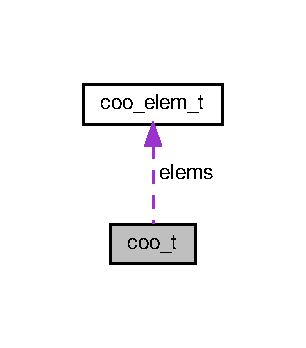
\includegraphics[width=147pt]{structcoo__t__coll__graph}
\end{center}
\end{figure}
\subsection*{Public Attributes}
\begin{DoxyCompactItemize}
\item 
\hyperlink{structcoo__elem__t}{coo\+\_\+elem\+\_\+t} $\ast$ \hyperlink{structcoo__t_a3e74f1e3dadd34e5439f859fab277b54}{elems}
\end{DoxyCompactItemize}


\subsection{Detailed Description}
sparse matrix in coodinate list format 

\subsection{Member Data Documentation}
\mbox{\Hypertarget{structcoo__t_a3e74f1e3dadd34e5439f859fab277b54}\label{structcoo__t_a3e74f1e3dadd34e5439f859fab277b54}} 
\index{coo\+\_\+t@{coo\+\_\+t}!elems@{elems}}
\index{elems@{elems}!coo\+\_\+t@{coo\+\_\+t}}
\subsubsection{\texorpdfstring{elems}{elems}}
{\footnotesize\ttfamily \hyperlink{structcoo__elem__t}{coo\+\_\+elem\+\_\+t}$\ast$ coo\+\_\+t\+::elems}

elements array 

The documentation for this struct was generated from the following file\+:\begin{DoxyCompactItemize}
\item 
/home/tau/public\+\_\+html/lecture/parallel\+\_\+distributed/2018/handson/tau/parallel-\/distributed-\/handson/03spmv/\hyperlink{spmv_8cc}{spmv.\+cc}\end{DoxyCompactItemize}

\hypertarget{structcsr__elem__t}{}\section{csr\+\_\+elem\+\_\+t Struct Reference}
\label{structcsr__elem__t}\index{csr\+\_\+elem\+\_\+t@{csr\+\_\+elem\+\_\+t}}


an element of compressed sparse row  


\subsection*{Public Attributes}
\begin{DoxyCompactItemize}
\item 
\hyperlink{spmv_8cc_a8e93478a00e685bea5e6a3f617bf03a3}{idx\+\_\+t} \hyperlink{structcsr__elem__t_a4525598ab26d6263b2242cc33511ca7f}{j}
\item 
\hyperlink{spmv_8cc_a11d147c64891830c9e79b3315b1b2e21}{real} \hyperlink{structcsr__elem__t_a55e480eefa495ee8b6e359a5f5a94a4f}{a}
\end{DoxyCompactItemize}


\subsection{Detailed Description}
an element of compressed sparse row 

\subsection{Member Data Documentation}
\mbox{\Hypertarget{structcsr__elem__t_a55e480eefa495ee8b6e359a5f5a94a4f}\label{structcsr__elem__t_a55e480eefa495ee8b6e359a5f5a94a4f}} 
\index{csr\+\_\+elem\+\_\+t@{csr\+\_\+elem\+\_\+t}!a@{a}}
\index{a@{a}!csr\+\_\+elem\+\_\+t@{csr\+\_\+elem\+\_\+t}}
\subsubsection{\texorpdfstring{a}{a}}
{\footnotesize\ttfamily \hyperlink{spmv_8cc_a11d147c64891830c9e79b3315b1b2e21}{real} csr\+\_\+elem\+\_\+t\+::a}

element \mbox{\Hypertarget{structcsr__elem__t_a4525598ab26d6263b2242cc33511ca7f}\label{structcsr__elem__t_a4525598ab26d6263b2242cc33511ca7f}} 
\index{csr\+\_\+elem\+\_\+t@{csr\+\_\+elem\+\_\+t}!j@{j}}
\index{j@{j}!csr\+\_\+elem\+\_\+t@{csr\+\_\+elem\+\_\+t}}
\subsubsection{\texorpdfstring{j}{j}}
{\footnotesize\ttfamily \hyperlink{spmv_8cc_a8e93478a00e685bea5e6a3f617bf03a3}{idx\+\_\+t} csr\+\_\+elem\+\_\+t\+::j}

column 

The documentation for this struct was generated from the following file\+:\begin{DoxyCompactItemize}
\item 
/home/tau/public\+\_\+html/lecture/parallel\+\_\+distributed/2018/parallel-\/distributed-\/handson/03spmv/\hyperlink{spmv_8cc}{spmv.\+cc}\end{DoxyCompactItemize}

\hypertarget{structcsr__t}{}\section{csr\+\_\+t Struct Reference}
\label{structcsr__t}\index{csr\+\_\+t@{csr\+\_\+t}}


sparse matrix in compressed row format  




Collaboration diagram for csr\+\_\+t\+:\nopagebreak
\begin{figure}[H]
\begin{center}
\leavevmode
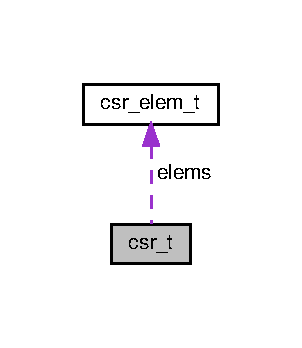
\includegraphics[width=145pt]{structcsr__t__coll__graph}
\end{center}
\end{figure}
\subsection*{Public Attributes}
\begin{DoxyCompactItemize}
\item 
\hyperlink{spmv_8cc_a8e93478a00e685bea5e6a3f617bf03a3}{idx\+\_\+t} $\ast$ \hyperlink{structcsr__t_ac52d7a1ff3a054e2b8c7fcc706e525b6}{row\+\_\+start}
\item 
\hyperlink{structcsr__elem__t}{csr\+\_\+elem\+\_\+t} $\ast$ \hyperlink{structcsr__t_a8fda532ad93e6820aad02feac6bbe04b}{elems}
\end{DoxyCompactItemize}


\subsection{Detailed Description}
sparse matrix in compressed row format 

\subsection{Member Data Documentation}
\mbox{\Hypertarget{structcsr__t_a8fda532ad93e6820aad02feac6bbe04b}\label{structcsr__t_a8fda532ad93e6820aad02feac6bbe04b}} 
\index{csr\+\_\+t@{csr\+\_\+t}!elems@{elems}}
\index{elems@{elems}!csr\+\_\+t@{csr\+\_\+t}}
\subsubsection{\texorpdfstring{elems}{elems}}
{\footnotesize\ttfamily \hyperlink{structcsr__elem__t}{csr\+\_\+elem\+\_\+t}$\ast$ csr\+\_\+t\+::elems}

elements array \mbox{\Hypertarget{structcsr__t_ac52d7a1ff3a054e2b8c7fcc706e525b6}\label{structcsr__t_ac52d7a1ff3a054e2b8c7fcc706e525b6}} 
\index{csr\+\_\+t@{csr\+\_\+t}!row\+\_\+start@{row\+\_\+start}}
\index{row\+\_\+start@{row\+\_\+start}!csr\+\_\+t@{csr\+\_\+t}}
\subsubsection{\texorpdfstring{row\+\_\+start}{row\_start}}
{\footnotesize\ttfamily \hyperlink{spmv_8cc_a8e93478a00e685bea5e6a3f617bf03a3}{idx\+\_\+t}$\ast$ csr\+\_\+t\+::row\+\_\+start}

elems\mbox{[}row\+\_\+start\mbox{[}i\mbox{]}\mbox{]} is the first element of row i 

The documentation for this struct was generated from the following file\+:\begin{DoxyCompactItemize}
\item 
/home/tau/public\+\_\+html/lecture/parallel\+\_\+distributed/2018/parallel-\/distributed-\/handson/03spmv/\hyperlink{spmv_8cc}{spmv.\+cc}\end{DoxyCompactItemize}

\hypertarget{structidx__pair__t}{}\section{idx\+\_\+pair\+\_\+t Struct Reference}
\label{structidx__pair__t}\index{idx\+\_\+pair\+\_\+t@{idx\+\_\+pair\+\_\+t}}


a pair of two indices (i and j)  


\subsection*{Public Attributes}
\begin{DoxyCompactItemize}
\item 
\hyperlink{spmv_8cc_a8e93478a00e685bea5e6a3f617bf03a3}{idx\+\_\+t} \hyperlink{structidx__pair__t_a5fc2a45497e05f6b02ae6dddd4cc5a14}{i}
\item 
\hyperlink{spmv_8cc_a8e93478a00e685bea5e6a3f617bf03a3}{idx\+\_\+t} \hyperlink{structidx__pair__t_afa260eb03684e5ae1c067c13fd33f3e0}{j}
\end{DoxyCompactItemize}


\subsection{Detailed Description}
a pair of two indices (i and j) 

\subsection{Member Data Documentation}
\mbox{\Hypertarget{structidx__pair__t_a5fc2a45497e05f6b02ae6dddd4cc5a14}\label{structidx__pair__t_a5fc2a45497e05f6b02ae6dddd4cc5a14}} 
\index{idx\+\_\+pair\+\_\+t@{idx\+\_\+pair\+\_\+t}!i@{i}}
\index{i@{i}!idx\+\_\+pair\+\_\+t@{idx\+\_\+pair\+\_\+t}}
\subsubsection{\texorpdfstring{i}{i}}
{\footnotesize\ttfamily \hyperlink{spmv_8cc_a8e93478a00e685bea5e6a3f617bf03a3}{idx\+\_\+t} idx\+\_\+pair\+\_\+t\+::i}

row number \mbox{\Hypertarget{structidx__pair__t_afa260eb03684e5ae1c067c13fd33f3e0}\label{structidx__pair__t_afa260eb03684e5ae1c067c13fd33f3e0}} 
\index{idx\+\_\+pair\+\_\+t@{idx\+\_\+pair\+\_\+t}!j@{j}}
\index{j@{j}!idx\+\_\+pair\+\_\+t@{idx\+\_\+pair\+\_\+t}}
\subsubsection{\texorpdfstring{j}{j}}
{\footnotesize\ttfamily \hyperlink{spmv_8cc_a8e93478a00e685bea5e6a3f617bf03a3}{idx\+\_\+t} idx\+\_\+pair\+\_\+t\+::j}

column number 

The documentation for this struct was generated from the following file\+:\begin{DoxyCompactItemize}
\item 
/home/tau/public\+\_\+html/lecture/parallel\+\_\+distributed/2018/parallel-\/distributed-\/handson/03spmv/\hyperlink{spmv_8cc}{spmv.\+cc}\end{DoxyCompactItemize}

\hypertarget{structimage__t}{}\section{image\+\_\+t Struct Reference}
\label{structimage__t}\index{image\+\_\+t@{image\+\_\+t}}


data structure through which to convert a matrix into a gnuplot file  


\subsection*{Public Attributes}
\begin{DoxyCompactItemize}
\item 
double $\ast$ \hyperlink{structimage__t_a2d2352a1d6c74a0df52a695bb3933d76}{a}
\item 
\hyperlink{spmv_8cc_a8e93478a00e685bea5e6a3f617bf03a3}{idx\+\_\+t} \hyperlink{structimage__t_a9ee57eb792a8c6bd1cd79efa329c728d}{M}
\item 
\hyperlink{spmv_8cc_a8e93478a00e685bea5e6a3f617bf03a3}{idx\+\_\+t} \hyperlink{structimage__t_ac6fdcfae13f4b5eccac7e9ef12502d64}{N}
\item 
\hyperlink{spmv_8cc_a8e93478a00e685bea5e6a3f617bf03a3}{idx\+\_\+t} \hyperlink{structimage__t_ae5f65c72e35caf8e730fe7962e732b0f}{img\+\_\+width}
\item 
\hyperlink{spmv_8cc_a8e93478a00e685bea5e6a3f617bf03a3}{idx\+\_\+t} \hyperlink{structimage__t_a37efb1b675fc28e5a131dca263fd2833}{img\+\_\+height}
\end{DoxyCompactItemize}


\subsection{Detailed Description}
data structure through which to convert a matrix into a gnuplot file 

\subsection{Member Data Documentation}
\mbox{\Hypertarget{structimage__t_a2d2352a1d6c74a0df52a695bb3933d76}\label{structimage__t_a2d2352a1d6c74a0df52a695bb3933d76}} 
\index{image\+\_\+t@{image\+\_\+t}!a@{a}}
\index{a@{a}!image\+\_\+t@{image\+\_\+t}}
\subsubsection{\texorpdfstring{a}{a}}
{\footnotesize\ttfamily double$\ast$ image\+\_\+t\+::a}

array of (img\+\_\+width x img\+\_\+height) elements \mbox{\Hypertarget{structimage__t_a37efb1b675fc28e5a131dca263fd2833}\label{structimage__t_a37efb1b675fc28e5a131dca263fd2833}} 
\index{image\+\_\+t@{image\+\_\+t}!img\+\_\+height@{img\+\_\+height}}
\index{img\+\_\+height@{img\+\_\+height}!image\+\_\+t@{image\+\_\+t}}
\subsubsection{\texorpdfstring{img\+\_\+height}{img\_height}}
{\footnotesize\ttfamily \hyperlink{spmv_8cc_a8e93478a00e685bea5e6a3f617bf03a3}{idx\+\_\+t} image\+\_\+t\+::img\+\_\+height}

number of vertial pixels (for M) \mbox{\Hypertarget{structimage__t_ae5f65c72e35caf8e730fe7962e732b0f}\label{structimage__t_ae5f65c72e35caf8e730fe7962e732b0f}} 
\index{image\+\_\+t@{image\+\_\+t}!img\+\_\+width@{img\+\_\+width}}
\index{img\+\_\+width@{img\+\_\+width}!image\+\_\+t@{image\+\_\+t}}
\subsubsection{\texorpdfstring{img\+\_\+width}{img\_width}}
{\footnotesize\ttfamily \hyperlink{spmv_8cc_a8e93478a00e685bea5e6a3f617bf03a3}{idx\+\_\+t} image\+\_\+t\+::img\+\_\+width}

number of horizontal pixels (for N) \mbox{\Hypertarget{structimage__t_a9ee57eb792a8c6bd1cd79efa329c728d}\label{structimage__t_a9ee57eb792a8c6bd1cd79efa329c728d}} 
\index{image\+\_\+t@{image\+\_\+t}!M@{M}}
\index{M@{M}!image\+\_\+t@{image\+\_\+t}}
\subsubsection{\texorpdfstring{M}{M}}
{\footnotesize\ttfamily \hyperlink{spmv_8cc_a8e93478a00e685bea5e6a3f617bf03a3}{idx\+\_\+t} image\+\_\+t\+::M}

the number of rows in the matrix \mbox{\Hypertarget{structimage__t_ac6fdcfae13f4b5eccac7e9ef12502d64}\label{structimage__t_ac6fdcfae13f4b5eccac7e9ef12502d64}} 
\index{image\+\_\+t@{image\+\_\+t}!N@{N}}
\index{N@{N}!image\+\_\+t@{image\+\_\+t}}
\subsubsection{\texorpdfstring{N}{N}}
{\footnotesize\ttfamily \hyperlink{spmv_8cc_a8e93478a00e685bea5e6a3f617bf03a3}{idx\+\_\+t} image\+\_\+t\+::N}

the number of columns in the matrix 

The documentation for this struct was generated from the following file\+:\begin{DoxyCompactItemize}
\item 
/home/tau/public\+\_\+html/lecture/parallel\+\_\+distributed/2018/parallel-\/distributed-\/handson/03spmv/\hyperlink{spmv_8cc}{spmv.\+cc}\end{DoxyCompactItemize}

\hypertarget{structsparse__format__table__entry__t}{}\section{sparse\+\_\+format\+\_\+table\+\_\+entry\+\_\+t Struct Reference}
\label{structsparse__format__table__entry__t}\index{sparse\+\_\+format\+\_\+table\+\_\+entry\+\_\+t@{sparse\+\_\+format\+\_\+table\+\_\+entry\+\_\+t}}


pair of the index value (sparse\+\_\+format\+\_\+t) and its name  


\subsection*{Public Attributes}
\begin{DoxyCompactItemize}
\item 
\hyperlink{spmv_8cc_a8c0094893526c01b430903b2d9227256}{sparse\+\_\+format\+\_\+t} \hyperlink{structsparse__format__table__entry__t_a1869dde0c0a30270a1f6477c01d530db}{idx}
\item 
const char $\ast$ \hyperlink{structsparse__format__table__entry__t_aff9c31fa7933890b2d4cf0f963df2d89}{name}
\end{DoxyCompactItemize}


\subsection{Detailed Description}
pair of the index value (sparse\+\_\+format\+\_\+t) and its name 

\subsection{Member Data Documentation}
\mbox{\Hypertarget{structsparse__format__table__entry__t_a1869dde0c0a30270a1f6477c01d530db}\label{structsparse__format__table__entry__t_a1869dde0c0a30270a1f6477c01d530db}} 
\index{sparse\+\_\+format\+\_\+table\+\_\+entry\+\_\+t@{sparse\+\_\+format\+\_\+table\+\_\+entry\+\_\+t}!idx@{idx}}
\index{idx@{idx}!sparse\+\_\+format\+\_\+table\+\_\+entry\+\_\+t@{sparse\+\_\+format\+\_\+table\+\_\+entry\+\_\+t}}
\subsubsection{\texorpdfstring{idx}{idx}}
{\footnotesize\ttfamily \hyperlink{spmv_8cc_a8c0094893526c01b430903b2d9227256}{sparse\+\_\+format\+\_\+t} sparse\+\_\+format\+\_\+table\+\_\+entry\+\_\+t\+::idx}

index value \mbox{\Hypertarget{structsparse__format__table__entry__t_aff9c31fa7933890b2d4cf0f963df2d89}\label{structsparse__format__table__entry__t_aff9c31fa7933890b2d4cf0f963df2d89}} 
\index{sparse\+\_\+format\+\_\+table\+\_\+entry\+\_\+t@{sparse\+\_\+format\+\_\+table\+\_\+entry\+\_\+t}!name@{name}}
\index{name@{name}!sparse\+\_\+format\+\_\+table\+\_\+entry\+\_\+t@{sparse\+\_\+format\+\_\+table\+\_\+entry\+\_\+t}}
\subsubsection{\texorpdfstring{name}{name}}
{\footnotesize\ttfamily const char$\ast$ sparse\+\_\+format\+\_\+table\+\_\+entry\+\_\+t\+::name}

name 

The documentation for this struct was generated from the following file\+:\begin{DoxyCompactItemize}
\item 
/home/tau/public\+\_\+html/lecture/parallel\+\_\+distributed/2018/parallel-\/distributed-\/handson/03spmv/\hyperlink{spmv_8cc}{spmv.\+cc}\end{DoxyCompactItemize}

\hypertarget{structsparse__format__table__t}{}\section{sparse\+\_\+format\+\_\+table\+\_\+t Struct Reference}
\label{structsparse__format__table__t}\index{sparse\+\_\+format\+\_\+table\+\_\+t@{sparse\+\_\+format\+\_\+table\+\_\+t}}


table of sparse format and their names  




Collaboration diagram for sparse\+\_\+format\+\_\+table\+\_\+t\+:\nopagebreak
\begin{figure}[H]
\begin{center}
\leavevmode
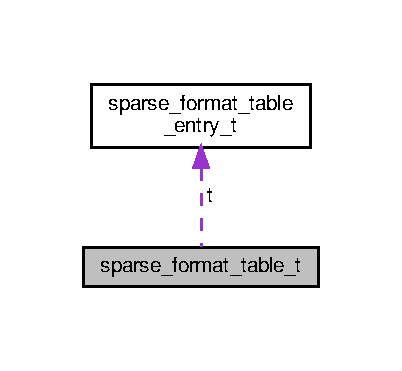
\includegraphics[width=193pt]{structsparse__format__table__t__coll__graph}
\end{center}
\end{figure}
\subsection*{Public Attributes}
\begin{DoxyCompactItemize}
\item 
\hyperlink{structsparse__format__table__entry__t}{sparse\+\_\+format\+\_\+table\+\_\+entry\+\_\+t} \hyperlink{structsparse__format__table__t_aded298a1583f5b097749cf84621c8ef4}{t} \mbox{[}\hyperlink{spmv_8cc_a8c0094893526c01b430903b2d9227256adc326179d0d559f82edc8cd35be11de5}{sparse\+\_\+format\+\_\+invalid}\mbox{]}
\end{DoxyCompactItemize}


\subsection{Detailed Description}
table of sparse format and their names 

\subsection{Member Data Documentation}
\mbox{\Hypertarget{structsparse__format__table__t_aded298a1583f5b097749cf84621c8ef4}\label{structsparse__format__table__t_aded298a1583f5b097749cf84621c8ef4}} 
\index{sparse\+\_\+format\+\_\+table\+\_\+t@{sparse\+\_\+format\+\_\+table\+\_\+t}!t@{t}}
\index{t@{t}!sparse\+\_\+format\+\_\+table\+\_\+t@{sparse\+\_\+format\+\_\+table\+\_\+t}}
\subsubsection{\texorpdfstring{t}{t}}
{\footnotesize\ttfamily \hyperlink{structsparse__format__table__entry__t}{sparse\+\_\+format\+\_\+table\+\_\+entry\+\_\+t} sparse\+\_\+format\+\_\+table\+\_\+t\+::t\mbox{[}\hyperlink{spmv_8cc_a8c0094893526c01b430903b2d9227256adc326179d0d559f82edc8cd35be11de5}{sparse\+\_\+format\+\_\+invalid}\mbox{]}}

array of index value -\/ name pairs 

The documentation for this struct was generated from the following file\+:\begin{DoxyCompactItemize}
\item 
/home/tau/public\+\_\+html/lecture/parallel\+\_\+distributed/2018/handson/tau/parallel-\/distributed-\/handson/03spmv/\hyperlink{spmv_8cc}{spmv.\+cc}\end{DoxyCompactItemize}

\hypertarget{structsparse__matrix__type__table__entry__t}{}\section{sparse\+\_\+matrix\+\_\+type\+\_\+table\+\_\+entry\+\_\+t Struct Reference}
\label{structsparse__matrix__type__table__entry__t}\index{sparse\+\_\+matrix\+\_\+type\+\_\+table\+\_\+entry\+\_\+t@{sparse\+\_\+matrix\+\_\+type\+\_\+table\+\_\+entry\+\_\+t}}


pair of the index value (matrix\+\_\+type\+\_\+t) and its name  


\subsection*{Public Attributes}
\begin{DoxyCompactItemize}
\item 
\hyperlink{spmv_8cc_a43a568fb26bc32aeaad07769cc524c45}{sparse\+\_\+matrix\+\_\+type\+\_\+t} \hyperlink{structsparse__matrix__type__table__entry__t_ae1bbdced2595c2b2e92a75b551631fc4}{idx}
\item 
const char $\ast$ \hyperlink{structsparse__matrix__type__table__entry__t_a7e2dea3171064e4ffece2e2c8a88c9ce}{name}
\end{DoxyCompactItemize}


\subsection{Detailed Description}
pair of the index value (matrix\+\_\+type\+\_\+t) and its name 

\subsection{Member Data Documentation}
\mbox{\Hypertarget{structsparse__matrix__type__table__entry__t_ae1bbdced2595c2b2e92a75b551631fc4}\label{structsparse__matrix__type__table__entry__t_ae1bbdced2595c2b2e92a75b551631fc4}} 
\index{sparse\+\_\+matrix\+\_\+type\+\_\+table\+\_\+entry\+\_\+t@{sparse\+\_\+matrix\+\_\+type\+\_\+table\+\_\+entry\+\_\+t}!idx@{idx}}
\index{idx@{idx}!sparse\+\_\+matrix\+\_\+type\+\_\+table\+\_\+entry\+\_\+t@{sparse\+\_\+matrix\+\_\+type\+\_\+table\+\_\+entry\+\_\+t}}
\subsubsection{\texorpdfstring{idx}{idx}}
{\footnotesize\ttfamily \hyperlink{spmv_8cc_a43a568fb26bc32aeaad07769cc524c45}{sparse\+\_\+matrix\+\_\+type\+\_\+t} sparse\+\_\+matrix\+\_\+type\+\_\+table\+\_\+entry\+\_\+t\+::idx}

index value \mbox{\Hypertarget{structsparse__matrix__type__table__entry__t_a7e2dea3171064e4ffece2e2c8a88c9ce}\label{structsparse__matrix__type__table__entry__t_a7e2dea3171064e4ffece2e2c8a88c9ce}} 
\index{sparse\+\_\+matrix\+\_\+type\+\_\+table\+\_\+entry\+\_\+t@{sparse\+\_\+matrix\+\_\+type\+\_\+table\+\_\+entry\+\_\+t}!name@{name}}
\index{name@{name}!sparse\+\_\+matrix\+\_\+type\+\_\+table\+\_\+entry\+\_\+t@{sparse\+\_\+matrix\+\_\+type\+\_\+table\+\_\+entry\+\_\+t}}
\subsubsection{\texorpdfstring{name}{name}}
{\footnotesize\ttfamily const char$\ast$ sparse\+\_\+matrix\+\_\+type\+\_\+table\+\_\+entry\+\_\+t\+::name}

name 

The documentation for this struct was generated from the following file\+:\begin{DoxyCompactItemize}
\item 
/home/tau/public\+\_\+html/lecture/parallel\+\_\+distributed/2018/handson/tau/parallel-\/distributed-\/handson/03spmv/\hyperlink{spmv_8cc}{spmv.\+cc}\end{DoxyCompactItemize}

\hypertarget{structsparse__matrix__type__table__t}{}\section{sparse\+\_\+matrix\+\_\+type\+\_\+table\+\_\+t Struct Reference}
\label{structsparse__matrix__type__table__t}\index{sparse\+\_\+matrix\+\_\+type\+\_\+table\+\_\+t@{sparse\+\_\+matrix\+\_\+type\+\_\+table\+\_\+t}}


table of sparse matrix types and their names  




Collaboration diagram for sparse\+\_\+matrix\+\_\+type\+\_\+table\+\_\+t\+:\nopagebreak
\begin{figure}[H]
\begin{center}
\leavevmode
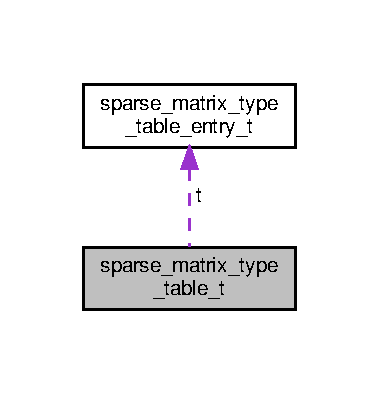
\includegraphics[width=182pt]{structsparse__matrix__type__table__t__coll__graph}
\end{center}
\end{figure}
\subsection*{Public Attributes}
\begin{DoxyCompactItemize}
\item 
\hyperlink{structsparse__matrix__type__table__entry__t}{sparse\+\_\+matrix\+\_\+type\+\_\+table\+\_\+entry\+\_\+t} \hyperlink{structsparse__matrix__type__table__t_a190c83be8b6111d25205a05ed0b23050}{t} \mbox{[}\hyperlink{spmv_8cc_a43a568fb26bc32aeaad07769cc524c45adbd59ebb0cfb220b9035a64fc2ed28dc}{sparse\+\_\+matrix\+\_\+type\+\_\+invalid}\mbox{]}
\end{DoxyCompactItemize}


\subsection{Detailed Description}
table of sparse matrix types and their names 

\subsection{Member Data Documentation}
\mbox{\Hypertarget{structsparse__matrix__type__table__t_a190c83be8b6111d25205a05ed0b23050}\label{structsparse__matrix__type__table__t_a190c83be8b6111d25205a05ed0b23050}} 
\index{sparse\+\_\+matrix\+\_\+type\+\_\+table\+\_\+t@{sparse\+\_\+matrix\+\_\+type\+\_\+table\+\_\+t}!t@{t}}
\index{t@{t}!sparse\+\_\+matrix\+\_\+type\+\_\+table\+\_\+t@{sparse\+\_\+matrix\+\_\+type\+\_\+table\+\_\+t}}
\subsubsection{\texorpdfstring{t}{t}}
{\footnotesize\ttfamily \hyperlink{structsparse__matrix__type__table__entry__t}{sparse\+\_\+matrix\+\_\+type\+\_\+table\+\_\+entry\+\_\+t} sparse\+\_\+matrix\+\_\+type\+\_\+table\+\_\+t\+::t\mbox{[}\hyperlink{spmv_8cc_a43a568fb26bc32aeaad07769cc524c45adbd59ebb0cfb220b9035a64fc2ed28dc}{sparse\+\_\+matrix\+\_\+type\+\_\+invalid}\mbox{]}}

array of index value -\/ name pairs 

The documentation for this struct was generated from the following file\+:\begin{DoxyCompactItemize}
\item 
/home/tau/public\+\_\+html/lecture/parallel\+\_\+distributed/2018/handson/tau/parallel-\/distributed-\/handson/03spmv/\hyperlink{spmv_8cc}{spmv.\+cc}\end{DoxyCompactItemize}

\hypertarget{structsparse__t}{}\section{sparse\+\_\+t Struct Reference}
\label{structsparse__t}\index{sparse\+\_\+t@{sparse\+\_\+t}}


sparse matrix (in any format)  




Collaboration diagram for sparse\+\_\+t\+:\nopagebreak
\begin{figure}[H]
\begin{center}
\leavevmode
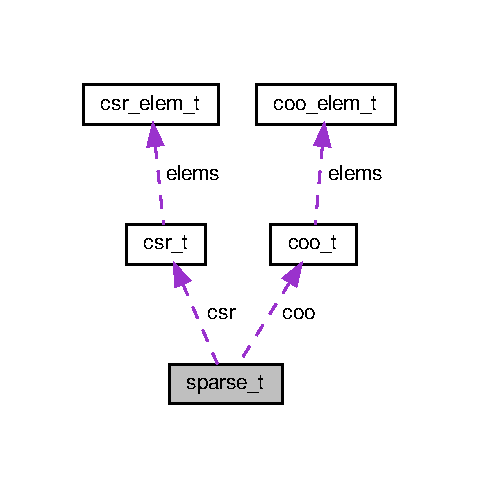
\includegraphics[width=230pt]{structsparse__t__coll__graph}
\end{center}
\end{figure}
\subsection*{Public Attributes}
\begin{DoxyCompactItemize}
\item 
\hyperlink{spmv_8cc_a8c0094893526c01b430903b2d9227256}{sparse\+\_\+format\+\_\+t} \hyperlink{structsparse__t_a1bb9e61c965f9ea814aab21f7ff77a73}{format}
\item 
\hyperlink{spmv_8cc_a8e93478a00e685bea5e6a3f617bf03a3}{idx\+\_\+t} \hyperlink{structsparse__t_a8a08bd7a16c76180afccf05e28f72a93}{M}
\item 
\hyperlink{spmv_8cc_a8e93478a00e685bea5e6a3f617bf03a3}{idx\+\_\+t} \hyperlink{structsparse__t_a418c6deef17a60f31ff11182ea94f85a}{N}
\item 
\hyperlink{spmv_8cc_a8e93478a00e685bea5e6a3f617bf03a3}{idx\+\_\+t} \hyperlink{structsparse__t_ae982d138f3904323b65975769b045a3f}{nnz}
\item 
\mbox{\Hypertarget{structsparse__t_a4d180146ce4a12b0d990cf0e803f7e64}\label{structsparse__t_a4d180146ce4a12b0d990cf0e803f7e64}} 
\begin{tabbing}
xx\=xx\=xx\=xx\=xx\=xx\=xx\=xx\=xx\=\kill
union \{\\
\>\hyperlink{structcoo__t}{coo\_t} \hyperlink{structsparse__t_ad0391f2782f49ea2eb248ed255e9d732}{coo}\\
\>\hyperlink{structcsr__t}{csr\_t} \hyperlink{structsparse__t_a68a71613181b0380d0d4d871236b2521}{csr}\\
\}; \\

\end{tabbing}\end{DoxyCompactItemize}


\subsection{Detailed Description}
sparse matrix (in any format) 

\subsection{Member Data Documentation}
\mbox{\Hypertarget{structsparse__t_ad0391f2782f49ea2eb248ed255e9d732}\label{structsparse__t_ad0391f2782f49ea2eb248ed255e9d732}} 
\index{sparse\+\_\+t@{sparse\+\_\+t}!coo@{coo}}
\index{coo@{coo}!sparse\+\_\+t@{sparse\+\_\+t}}
\subsubsection{\texorpdfstring{coo}{coo}}
{\footnotesize\ttfamily \hyperlink{structcoo__t}{coo\+\_\+t} sparse\+\_\+t\+::coo}

coo or sorted coo \mbox{\Hypertarget{structsparse__t_a68a71613181b0380d0d4d871236b2521}\label{structsparse__t_a68a71613181b0380d0d4d871236b2521}} 
\index{sparse\+\_\+t@{sparse\+\_\+t}!csr@{csr}}
\index{csr@{csr}!sparse\+\_\+t@{sparse\+\_\+t}}
\subsubsection{\texorpdfstring{csr}{csr}}
{\footnotesize\ttfamily \hyperlink{structcsr__t}{csr\+\_\+t} sparse\+\_\+t\+::csr}

csr \mbox{\Hypertarget{structsparse__t_a1bb9e61c965f9ea814aab21f7ff77a73}\label{structsparse__t_a1bb9e61c965f9ea814aab21f7ff77a73}} 
\index{sparse\+\_\+t@{sparse\+\_\+t}!format@{format}}
\index{format@{format}!sparse\+\_\+t@{sparse\+\_\+t}}
\subsubsection{\texorpdfstring{format}{format}}
{\footnotesize\ttfamily \hyperlink{spmv_8cc_a8c0094893526c01b430903b2d9227256}{sparse\+\_\+format\+\_\+t} sparse\+\_\+t\+::format}

format \mbox{\Hypertarget{structsparse__t_a8a08bd7a16c76180afccf05e28f72a93}\label{structsparse__t_a8a08bd7a16c76180afccf05e28f72a93}} 
\index{sparse\+\_\+t@{sparse\+\_\+t}!M@{M}}
\index{M@{M}!sparse\+\_\+t@{sparse\+\_\+t}}
\subsubsection{\texorpdfstring{M}{M}}
{\footnotesize\ttfamily \hyperlink{spmv_8cc_a8e93478a00e685bea5e6a3f617bf03a3}{idx\+\_\+t} sparse\+\_\+t\+::M}

number of rows \mbox{\Hypertarget{structsparse__t_a418c6deef17a60f31ff11182ea94f85a}\label{structsparse__t_a418c6deef17a60f31ff11182ea94f85a}} 
\index{sparse\+\_\+t@{sparse\+\_\+t}!N@{N}}
\index{N@{N}!sparse\+\_\+t@{sparse\+\_\+t}}
\subsubsection{\texorpdfstring{N}{N}}
{\footnotesize\ttfamily \hyperlink{spmv_8cc_a8e93478a00e685bea5e6a3f617bf03a3}{idx\+\_\+t} sparse\+\_\+t\+::N}

number of columns \mbox{\Hypertarget{structsparse__t_ae982d138f3904323b65975769b045a3f}\label{structsparse__t_ae982d138f3904323b65975769b045a3f}} 
\index{sparse\+\_\+t@{sparse\+\_\+t}!nnz@{nnz}}
\index{nnz@{nnz}!sparse\+\_\+t@{sparse\+\_\+t}}
\subsubsection{\texorpdfstring{nnz}{nnz}}
{\footnotesize\ttfamily \hyperlink{spmv_8cc_a8e93478a00e685bea5e6a3f617bf03a3}{idx\+\_\+t} sparse\+\_\+t\+::nnz}

number of non-\/zeros 

The documentation for this struct was generated from the following file\+:\begin{DoxyCompactItemize}
\item 
/home/tau/public\+\_\+html/lecture/parallel\+\_\+distributed/2018/parallel-\/distributed-\/handson/03spmv/\hyperlink{spmv_8cc}{spmv.\+cc}\end{DoxyCompactItemize}

\hypertarget{structspmv__algo__table__entry__t}{}\section{spmv\+\_\+algo\+\_\+table\+\_\+entry\+\_\+t Struct Reference}
\label{structspmv__algo__table__entry__t}\index{spmv\+\_\+algo\+\_\+table\+\_\+entry\+\_\+t@{spmv\+\_\+algo\+\_\+table\+\_\+entry\+\_\+t}}


pair of the index value (spmv\+\_\+algo\+\_\+t) and its name  


\subsection*{Public Attributes}
\begin{DoxyCompactItemize}
\item 
\hyperlink{spmv_8cc_ad2cf0493af54bf76c5be68b4634fcab7}{spmv\+\_\+algo\+\_\+t} \hyperlink{structspmv__algo__table__entry__t_a0ef60703788aaa74667e3bec5f44696d}{idx}
\item 
const char $\ast$ \hyperlink{structspmv__algo__table__entry__t_a0d9006dae288632b43113eeef8aa9f11}{name}
\end{DoxyCompactItemize}


\subsection{Detailed Description}
pair of the index value (spmv\+\_\+algo\+\_\+t) and its name 

\subsection{Member Data Documentation}
\mbox{\Hypertarget{structspmv__algo__table__entry__t_a0ef60703788aaa74667e3bec5f44696d}\label{structspmv__algo__table__entry__t_a0ef60703788aaa74667e3bec5f44696d}} 
\index{spmv\+\_\+algo\+\_\+table\+\_\+entry\+\_\+t@{spmv\+\_\+algo\+\_\+table\+\_\+entry\+\_\+t}!idx@{idx}}
\index{idx@{idx}!spmv\+\_\+algo\+\_\+table\+\_\+entry\+\_\+t@{spmv\+\_\+algo\+\_\+table\+\_\+entry\+\_\+t}}
\subsubsection{\texorpdfstring{idx}{idx}}
{\footnotesize\ttfamily \hyperlink{spmv_8cc_ad2cf0493af54bf76c5be68b4634fcab7}{spmv\+\_\+algo\+\_\+t} spmv\+\_\+algo\+\_\+table\+\_\+entry\+\_\+t\+::idx}

index value \mbox{\Hypertarget{structspmv__algo__table__entry__t_a0d9006dae288632b43113eeef8aa9f11}\label{structspmv__algo__table__entry__t_a0d9006dae288632b43113eeef8aa9f11}} 
\index{spmv\+\_\+algo\+\_\+table\+\_\+entry\+\_\+t@{spmv\+\_\+algo\+\_\+table\+\_\+entry\+\_\+t}!name@{name}}
\index{name@{name}!spmv\+\_\+algo\+\_\+table\+\_\+entry\+\_\+t@{spmv\+\_\+algo\+\_\+table\+\_\+entry\+\_\+t}}
\subsubsection{\texorpdfstring{name}{name}}
{\footnotesize\ttfamily const char$\ast$ spmv\+\_\+algo\+\_\+table\+\_\+entry\+\_\+t\+::name}

name 

The documentation for this struct was generated from the following file\+:\begin{DoxyCompactItemize}
\item 
/home/tau/public\+\_\+html/lecture/parallel\+\_\+distributed/2018/handson/tau/parallel-\/distributed-\/handson/03spmv/\hyperlink{spmv_8cc}{spmv.\+cc}\end{DoxyCompactItemize}

\hypertarget{structspmv__algo__table__t}{}\section{spmv\+\_\+algo\+\_\+table\+\_\+t Struct Reference}
\label{structspmv__algo__table__t}\index{spmv\+\_\+algo\+\_\+table\+\_\+t@{spmv\+\_\+algo\+\_\+table\+\_\+t}}


table of spmv algorithms and their names  




Collaboration diagram for spmv\+\_\+algo\+\_\+table\+\_\+t\+:\nopagebreak
\begin{figure}[H]
\begin{center}
\leavevmode
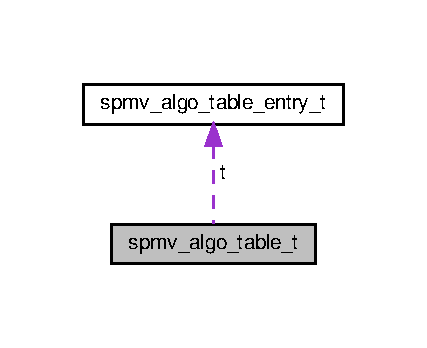
\includegraphics[width=205pt]{structspmv__algo__table__t__coll__graph}
\end{center}
\end{figure}
\subsection*{Public Attributes}
\begin{DoxyCompactItemize}
\item 
\hyperlink{structspmv__algo__table__entry__t}{spmv\+\_\+algo\+\_\+table\+\_\+entry\+\_\+t} \hyperlink{structspmv__algo__table__t_a8cc8ce6a17f236df757787d28ae93315}{t} \mbox{[}\hyperlink{spmv_8cc_ad2cf0493af54bf76c5be68b4634fcab7add2a1e0329d677ee5f5fcc7ee8077dd0}{spmv\+\_\+algo\+\_\+invalid}\mbox{]}
\end{DoxyCompactItemize}


\subsection{Detailed Description}
table of spmv algorithms and their names 

\subsection{Member Data Documentation}
\mbox{\Hypertarget{structspmv__algo__table__t_a8cc8ce6a17f236df757787d28ae93315}\label{structspmv__algo__table__t_a8cc8ce6a17f236df757787d28ae93315}} 
\index{spmv\+\_\+algo\+\_\+table\+\_\+t@{spmv\+\_\+algo\+\_\+table\+\_\+t}!t@{t}}
\index{t@{t}!spmv\+\_\+algo\+\_\+table\+\_\+t@{spmv\+\_\+algo\+\_\+table\+\_\+t}}
\subsubsection{\texorpdfstring{t}{t}}
{\footnotesize\ttfamily \hyperlink{structspmv__algo__table__entry__t}{spmv\+\_\+algo\+\_\+table\+\_\+entry\+\_\+t} spmv\+\_\+algo\+\_\+table\+\_\+t\+::t\mbox{[}\hyperlink{spmv_8cc_ad2cf0493af54bf76c5be68b4634fcab7add2a1e0329d677ee5f5fcc7ee8077dd0}{spmv\+\_\+algo\+\_\+invalid}\mbox{]}}

array of index value -\/ name pairs 

The documentation for this struct was generated from the following file\+:\begin{DoxyCompactItemize}
\item 
/home/tau/public\+\_\+html/lecture/parallel\+\_\+distributed/2018/parallel-\/distributed-\/handson/03spmv/\hyperlink{spmv_8cc}{spmv.\+cc}\end{DoxyCompactItemize}

\hypertarget{structvec__t}{}\section{vec\+\_\+t Struct Reference}
\label{structvec__t}\index{vec\+\_\+t@{vec\+\_\+t}}


vector  


\subsection*{Public Attributes}
\begin{DoxyCompactItemize}
\item 
\hyperlink{spmv_8cc_a8e93478a00e685bea5e6a3f617bf03a3}{idx\+\_\+t} \hyperlink{structvec__t_a06879ff4054298fbc680b02e3e18da7a}{n}
\item 
\hyperlink{spmv_8cc_a11d147c64891830c9e79b3315b1b2e21}{real} $\ast$ \hyperlink{structvec__t_af9bc087be96662c10187c01cf9bfc834}{elems}
\end{DoxyCompactItemize}


\subsection{Detailed Description}
vector 

\subsection{Member Data Documentation}
\mbox{\Hypertarget{structvec__t_af9bc087be96662c10187c01cf9bfc834}\label{structvec__t_af9bc087be96662c10187c01cf9bfc834}} 
\index{vec\+\_\+t@{vec\+\_\+t}!elems@{elems}}
\index{elems@{elems}!vec\+\_\+t@{vec\+\_\+t}}
\subsubsection{\texorpdfstring{elems}{elems}}
{\footnotesize\ttfamily \hyperlink{spmv_8cc_a11d147c64891830c9e79b3315b1b2e21}{real} $\ast$ vec\+\_\+t\+::elems}

array of elements \mbox{\Hypertarget{structvec__t_a06879ff4054298fbc680b02e3e18da7a}\label{structvec__t_a06879ff4054298fbc680b02e3e18da7a}} 
\index{vec\+\_\+t@{vec\+\_\+t}!n@{n}}
\index{n@{n}!vec\+\_\+t@{vec\+\_\+t}}
\subsubsection{\texorpdfstring{n}{n}}
{\footnotesize\ttfamily \hyperlink{spmv_8cc_a8e93478a00e685bea5e6a3f617bf03a3}{idx\+\_\+t} vec\+\_\+t\+::n}

number of elements 

The documentation for this struct was generated from the following files\+:\begin{DoxyCompactItemize}
\item 
/home/tau/public\+\_\+html/lecture/parallel\+\_\+distributed/2018/parallel-\/distributed-\/handson/03spmv/\hyperlink{spmv_8cc}{spmv.\+cc}\item 
/home/tau/public\+\_\+html/lecture/parallel\+\_\+distributed/2018/parallel-\/distributed-\/handson/03spmv/spmvx.\+cc\end{DoxyCompactItemize}

\chapter{File Documentation}
\hypertarget{cuda__util_8h}{}\section{/home/tau/public\+\_\+html/lecture/parallel\+\_\+distributed/2018/parallel-\/distributed-\/handson/03spmv/cuda\+\_\+util.h File Reference}
\label{cuda__util_8h}\index{/home/tau/public\+\_\+html/lecture/parallel\+\_\+distributed/2018/parallel-\/distributed-\/handson/03spmv/cuda\+\_\+util.\+h@{/home/tau/public\+\_\+html/lecture/parallel\+\_\+distributed/2018/parallel-\/distributed-\/handson/03spmv/cuda\+\_\+util.\+h}}


small utility functions for cuda  


\subsection*{Macros}
\begin{DoxyCompactItemize}
\item 
\#define \hyperlink{cuda__util_8h_ae08da20e750e9eabdf37c5cdf87a6e73}{check\+\_\+api\+\_\+error}(e)~check\+\_\+api\+\_\+error\+\_\+(e, \#e, \+\_\+\+\_\+\+F\+I\+L\+E\+\_\+\+\_\+, \+\_\+\+\_\+\+L\+I\+N\+E\+\_\+\+\_\+)
\begin{DoxyCompactList}\small\item\em check if a C\+U\+DA A\+PI invocation succeeded and show the error msg if any \end{DoxyCompactList}\item 
\#define \hyperlink{cuda__util_8h_ae8a9e1ffcd7af83a818bc9a6ec7bed78}{check\+\_\+launch\+\_\+error}(exp)~do \{ exp; check\+\_\+kernel\+\_\+error\+\_\+(\#exp, \+\_\+\+\_\+\+F\+I\+L\+E\+\_\+\+\_\+, \+\_\+\+\_\+\+L\+I\+N\+E\+\_\+\+\_\+); \} while (0)
\begin{DoxyCompactList}\small\item\em check kernel invocation error \end{DoxyCompactList}\end{DoxyCompactItemize}
\subsection*{Functions}
\begin{DoxyCompactItemize}
\item 
\mbox{\Hypertarget{cuda__util_8h_a42ba739c08e201d58f7a031d899a0e7f}\label{cuda__util_8h_a42ba739c08e201d58f7a031d899a0e7f}} 
\+\_\+\+\_\+device\+\_\+\+\_\+ uint \hyperlink{cuda__util_8h_a42ba739c08e201d58f7a031d899a0e7f}{get\+\_\+smid} (void)
\begin{DoxyCompactList}\small\item\em get SM executing the caller \end{DoxyCompactList}\item 
\mbox{\Hypertarget{cuda__util_8h_a0737678a7fc54cb0347e3c4178ad5dfa}\label{cuda__util_8h_a0737678a7fc54cb0347e3c4178ad5dfa}} 
void \hyperlink{cuda__util_8h_a0737678a7fc54cb0347e3c4178ad5dfa}{to\+\_\+host} (void $\ast$dst, void $\ast$src, size\+\_\+t sz)
\begin{DoxyCompactList}\small\item\em wrap cuda\+Memcpy to copy from device to host (and check an error if any) \end{DoxyCompactList}\item 
\mbox{\Hypertarget{cuda__util_8h_a30655f0f077528b999634c85513af4b0}\label{cuda__util_8h_a30655f0f077528b999634c85513af4b0}} 
\+\_\+\+\_\+device\+\_\+\+\_\+ int \hyperlink{cuda__util_8h_a30655f0f077528b999634c85513af4b0}{get\+\_\+thread\+\_\+id\+\_\+x} ()
\begin{DoxyCompactList}\small\item\em thread ID along x-\/dimension \end{DoxyCompactList}\item 
\mbox{\Hypertarget{cuda__util_8h_a6ea184310bf6fc2e1313127215aab5b0}\label{cuda__util_8h_a6ea184310bf6fc2e1313127215aab5b0}} 
\+\_\+\+\_\+device\+\_\+\+\_\+ int \hyperlink{cuda__util_8h_a6ea184310bf6fc2e1313127215aab5b0}{get\+\_\+thread\+\_\+id\+\_\+y} ()
\begin{DoxyCompactList}\small\item\em thread ID along y-\/dimension \end{DoxyCompactList}\item 
\mbox{\Hypertarget{cuda__util_8h_afff8c5c6d0e85b4a264786a4170ad777}\label{cuda__util_8h_afff8c5c6d0e85b4a264786a4170ad777}} 
\+\_\+\+\_\+device\+\_\+\+\_\+ int \hyperlink{cuda__util_8h_afff8c5c6d0e85b4a264786a4170ad777}{get\+\_\+thread\+\_\+id\+\_\+z} ()
\begin{DoxyCompactList}\small\item\em thread ID along z-\/dimension \end{DoxyCompactList}\item 
\mbox{\Hypertarget{cuda__util_8h_ae13980c33ac8f950ed35d613415034c0}\label{cuda__util_8h_ae13980c33ac8f950ed35d613415034c0}} 
\+\_\+\+\_\+device\+\_\+\+\_\+ int \hyperlink{cuda__util_8h_ae13980c33ac8f950ed35d613415034c0}{get\+\_\+nthreads\+\_\+x} ()
\begin{DoxyCompactList}\small\item\em number of threads along x-\/dimension \end{DoxyCompactList}\item 
\mbox{\Hypertarget{cuda__util_8h_a79fd9ff68db3a81b8b0feb446e4e9b99}\label{cuda__util_8h_a79fd9ff68db3a81b8b0feb446e4e9b99}} 
\+\_\+\+\_\+device\+\_\+\+\_\+ int \hyperlink{cuda__util_8h_a79fd9ff68db3a81b8b0feb446e4e9b99}{get\+\_\+nthreads\+\_\+y} ()
\begin{DoxyCompactList}\small\item\em number of threads along y-\/dimension \end{DoxyCompactList}\item 
\mbox{\Hypertarget{cuda__util_8h_a59cd23ec9bc1ab07e3eaac1ad3e109b4}\label{cuda__util_8h_a59cd23ec9bc1ab07e3eaac1ad3e109b4}} 
\+\_\+\+\_\+device\+\_\+\+\_\+ int \hyperlink{cuda__util_8h_a59cd23ec9bc1ab07e3eaac1ad3e109b4}{get\+\_\+nthreads\+\_\+z} ()
\begin{DoxyCompactList}\small\item\em number of threads along z-\/dimension \end{DoxyCompactList}\item 
\mbox{\Hypertarget{cuda__util_8h_ace44c6e6794929ce9e48e1122c7a3a12}\label{cuda__util_8h_ace44c6e6794929ce9e48e1122c7a3a12}} 
\+\_\+\+\_\+device\+\_\+\+\_\+ int \hyperlink{cuda__util_8h_ace44c6e6794929ce9e48e1122c7a3a12}{get\+\_\+thread\+\_\+id} ()
\begin{DoxyCompactList}\small\item\em global (x,y,z combined into an integer) thread ID \end{DoxyCompactList}\item 
\mbox{\Hypertarget{cuda__util_8h_a74d008c0d996e10f203bdd1fdee76511}\label{cuda__util_8h_a74d008c0d996e10f203bdd1fdee76511}} 
\+\_\+\+\_\+device\+\_\+\+\_\+ int \hyperlink{cuda__util_8h_a74d008c0d996e10f203bdd1fdee76511}{get\+\_\+nthreads} ()
\begin{DoxyCompactList}\small\item\em total number of threads \end{DoxyCompactList}\end{DoxyCompactItemize}


\subsection{Detailed Description}
small utility functions for cuda 

\begin{DoxyAuthor}{Author}
Kenjiro Taura 
\end{DoxyAuthor}
\begin{DoxyDate}{Date}
Oct. 14, 2018 
\end{DoxyDate}


\subsection{Macro Definition Documentation}
\mbox{\Hypertarget{cuda__util_8h_ae08da20e750e9eabdf37c5cdf87a6e73}\label{cuda__util_8h_ae08da20e750e9eabdf37c5cdf87a6e73}} 
\index{cuda\+\_\+util.\+h@{cuda\+\_\+util.\+h}!check\+\_\+api\+\_\+error@{check\+\_\+api\+\_\+error}}
\index{check\+\_\+api\+\_\+error@{check\+\_\+api\+\_\+error}!cuda\+\_\+util.\+h@{cuda\+\_\+util.\+h}}
\subsubsection{\texorpdfstring{check\+\_\+api\+\_\+error}{check\_api\_error}}
{\footnotesize\ttfamily \#define check\+\_\+api\+\_\+error(\begin{DoxyParamCaption}\item[{}]{e }\end{DoxyParamCaption})~check\+\_\+api\+\_\+error\+\_\+(e, \#e, \+\_\+\+\_\+\+F\+I\+L\+E\+\_\+\+\_\+, \+\_\+\+\_\+\+L\+I\+N\+E\+\_\+\+\_\+)}



check if a C\+U\+DA A\+PI invocation succeeded and show the error msg if any 

usage\+: check\+\_\+cuda\+\_\+error(cuda\+\_\+api\+\_\+call()). for example, check\+\_\+cuda\+\_\+error(cuda\+Malloc(\&p, size)); \mbox{\Hypertarget{cuda__util_8h_ae8a9e1ffcd7af83a818bc9a6ec7bed78}\label{cuda__util_8h_ae8a9e1ffcd7af83a818bc9a6ec7bed78}} 
\index{cuda\+\_\+util.\+h@{cuda\+\_\+util.\+h}!check\+\_\+launch\+\_\+error@{check\+\_\+launch\+\_\+error}}
\index{check\+\_\+launch\+\_\+error@{check\+\_\+launch\+\_\+error}!cuda\+\_\+util.\+h@{cuda\+\_\+util.\+h}}
\subsubsection{\texorpdfstring{check\+\_\+launch\+\_\+error}{check\_launch\_error}}
{\footnotesize\ttfamily \#define check\+\_\+launch\+\_\+error(\begin{DoxyParamCaption}\item[{}]{exp }\end{DoxyParamCaption})~do \{ exp; check\+\_\+kernel\+\_\+error\+\_\+(\#exp, \+\_\+\+\_\+\+F\+I\+L\+E\+\_\+\+\_\+, \+\_\+\+\_\+\+L\+I\+N\+E\+\_\+\+\_\+); \} while (0)}



check kernel invocation error 

usage\+: check\+\_\+kernel\+\_\+error((kernel-\/launch-\/expression)). for example, check\+\_\+kernel\+\_\+error((your\+\_\+gpu\+\_\+kernel$<$$<$$<$n\+\_\+blocks,block\+\_\+sz$>$$>$$>$(a,b,c))). note that you need to put parens around the expression. 
\hypertarget{spmv_8cc}{}\section{/home/tau/public\+\_\+html/lecture/parallel\+\_\+distributed/2018/ex/00spmv/spmv.cc File Reference}
\label{spmv_8cc}\index{/home/tau/public\+\_\+html/lecture/parallel\+\_\+distributed/2018/ex/00spmv/spmv.\+cc@{/home/tau/public\+\_\+html/lecture/parallel\+\_\+distributed/2018/ex/00spmv/spmv.\+cc}}


sparse matrix vector multiplication  


{\ttfamily \#include $<$assert.\+h$>$}\newline
{\ttfamily \#include $<$math.\+h$>$}\newline
{\ttfamily \#include $<$stdio.\+h$>$}\newline
{\ttfamily \#include $<$stdlib.\+h$>$}\newline
{\ttfamily \#include $<$string.\+h$>$}\newline
{\ttfamily \#include $<$getopt.\+h$>$}\newline
{\ttfamily \#include $<$time.\+h$>$}\newline
Include dependency graph for spmv.\+cc\+:
\nopagebreak
\begin{figure}[H]
\begin{center}
\leavevmode
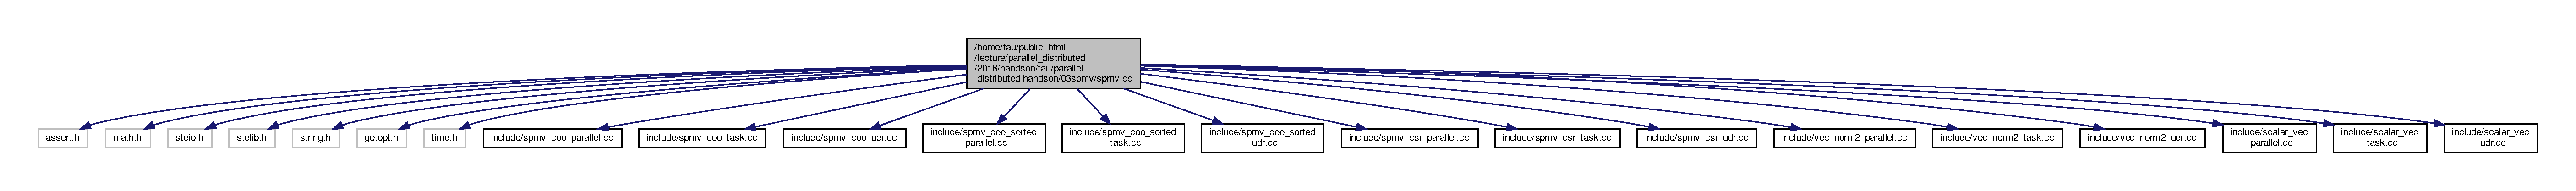
\includegraphics[width=350pt]{spmv_8cc__incl}
\end{center}
\end{figure}
\subsection*{Classes}
\begin{DoxyCompactItemize}
\item 
struct \hyperlink{structcoo__elem__t}{coo\+\_\+elem\+\_\+t}
\begin{DoxyCompactList}\small\item\em an element of coordinate list (i, j, a) \end{DoxyCompactList}\item 
struct \hyperlink{structcsr__elem__t}{csr\+\_\+elem\+\_\+t}
\begin{DoxyCompactList}\small\item\em an element of compressed sparse row \end{DoxyCompactList}\item 
struct \hyperlink{structcoo__t}{coo\+\_\+t}
\begin{DoxyCompactList}\small\item\em sparse matrix in coodinate list format \end{DoxyCompactList}\item 
struct \hyperlink{structcsr__t}{csr\+\_\+t}
\begin{DoxyCompactList}\small\item\em sparse matrix in compressed row format \end{DoxyCompactList}\item 
struct \hyperlink{structsparse__t}{sparse\+\_\+t}
\begin{DoxyCompactList}\small\item\em sparse matrix (in any format) \end{DoxyCompactList}\item 
struct \hyperlink{structvec__t}{vec\+\_\+t}
\begin{DoxyCompactList}\small\item\em vector \end{DoxyCompactList}\item 
struct \hyperlink{structcmdline__options__t}{cmdline\+\_\+options\+\_\+t}
\begin{DoxyCompactList}\small\item\em command line option \end{DoxyCompactList}\end{DoxyCompactItemize}
\subsection*{Typedefs}
\begin{DoxyCompactItemize}
\item 
\mbox{\Hypertarget{spmv_8cc_a8e93478a00e685bea5e6a3f617bf03a3}\label{spmv_8cc_a8e93478a00e685bea5e6a3f617bf03a3}} 
typedef int \hyperlink{spmv_8cc_a8e93478a00e685bea5e6a3f617bf03a3}{idx\+\_\+t}
\begin{DoxyCompactList}\small\item\em type of matrix index (i,j,...) \end{DoxyCompactList}\item 
\mbox{\Hypertarget{spmv_8cc_a11d147c64891830c9e79b3315b1b2e21}\label{spmv_8cc_a11d147c64891830c9e79b3315b1b2e21}} 
typedef double \hyperlink{spmv_8cc_a11d147c64891830c9e79b3315b1b2e21}{real}
\begin{DoxyCompactList}\small\item\em type of a matrix element \end{DoxyCompactList}\end{DoxyCompactItemize}
\subsection*{Enumerations}
\begin{DoxyCompactItemize}
\item 
enum \hyperlink{spmv_8cc_a8c0094893526c01b430903b2d9227256}{sparse\+\_\+format\+\_\+t} \{ \hyperlink{spmv_8cc_a8c0094893526c01b430903b2d9227256a3873dfc9b4303f69130d325bb9d5d3d9}{sparse\+\_\+format\+\_\+coo}, 
\hyperlink{spmv_8cc_a8c0094893526c01b430903b2d9227256ae622b3c6575c5efae6930339af50e076}{sparse\+\_\+format\+\_\+coo\+\_\+sorted}, 
\hyperlink{spmv_8cc_a8c0094893526c01b430903b2d9227256a8d3a61cb0ac76c8b5334c24c7618c4c7}{sparse\+\_\+format\+\_\+csr}, 
\hyperlink{spmv_8cc_a8c0094893526c01b430903b2d9227256adc326179d0d559f82edc8cd35be11de5}{sparse\+\_\+format\+\_\+invalid}
 \}\begin{DoxyCompactList}\small\item\em sparse matrix storage format \end{DoxyCompactList}
\item 
enum \hyperlink{spmv_8cc_ad2cf0493af54bf76c5be68b4634fcab7}{spmv\+\_\+algo\+\_\+t} \{ \hyperlink{spmv_8cc_ad2cf0493af54bf76c5be68b4634fcab7a8239a128e5970e7f36aec71d6265d78a}{spmv\+\_\+algo\+\_\+serial}, 
\hyperlink{spmv_8cc_ad2cf0493af54bf76c5be68b4634fcab7abbdcd58ce962bc8134af08a7f4310f81}{spmv\+\_\+algo\+\_\+parallel}, 
{\bfseries spmv\+\_\+algo\+\_\+invalid}
 \}\begin{DoxyCompactList}\small\item\em spmv matrix algorithm \end{DoxyCompactList}
\end{DoxyCompactItemize}
\subsection*{Functions}
\begin{DoxyCompactItemize}
\item 
\mbox{\Hypertarget{spmv_8cc_a79a33f2f3ea6bfd4bd5fc8bc1c026a5b}\label{spmv_8cc_a79a33f2f3ea6bfd4bd5fc8bc1c026a5b}} 
void $\ast$ \hyperlink{spmv_8cc_a79a33f2f3ea6bfd4bd5fc8bc1c026a5b}{xalloc} (size\+\_\+t sz)
\begin{DoxyCompactList}\small\item\em malloc + check \end{DoxyCompactList}\item 
\mbox{\Hypertarget{spmv_8cc_a3ef938bd87c574f4deb4e5b05de27fc2}\label{spmv_8cc_a3ef938bd87c574f4deb4e5b05de27fc2}} 
void \hyperlink{spmv_8cc_a3ef938bd87c574f4deb4e5b05de27fc2}{xfree} (void $\ast$a)
\begin{DoxyCompactList}\small\item\em wrap free \end{DoxyCompactList}\item 
\mbox{\Hypertarget{spmv_8cc_a886d462f047a9680c3a5b9359a082469}\label{spmv_8cc_a886d462f047a9680c3a5b9359a082469}} 
void \hyperlink{spmv_8cc_a886d462f047a9680c3a5b9359a082469}{coo\+\_\+destroy} (\hyperlink{structsparse__t}{sparse\+\_\+t} A)
\begin{DoxyCompactList}\small\item\em destroy coo \end{DoxyCompactList}\item 
\mbox{\Hypertarget{spmv_8cc_a3ae3b530bd4c6af7148b8d6f0350d5b7}\label{spmv_8cc_a3ae3b530bd4c6af7148b8d6f0350d5b7}} 
void \hyperlink{spmv_8cc_a3ae3b530bd4c6af7148b8d6f0350d5b7}{csr\+\_\+destroy} (\hyperlink{structsparse__t}{sparse\+\_\+t} A)
\begin{DoxyCompactList}\small\item\em destroy csr \end{DoxyCompactList}\item 
\mbox{\Hypertarget{spmv_8cc_a9743d89de22a2978402684c73921c2f7}\label{spmv_8cc_a9743d89de22a2978402684c73921c2f7}} 
void \hyperlink{spmv_8cc_a9743d89de22a2978402684c73921c2f7}{sparse\+\_\+destroy} (\hyperlink{structsparse__t}{sparse\+\_\+t} A)
\begin{DoxyCompactList}\small\item\em destroy sparse matrix in any format \end{DoxyCompactList}\item 
\mbox{\Hypertarget{spmv_8cc_a174b34f4428f02a25bcaf8bb40309198}\label{spmv_8cc_a174b34f4428f02a25bcaf8bb40309198}} 
void \hyperlink{spmv_8cc_a174b34f4428f02a25bcaf8bb40309198}{vec\+\_\+destroy} (\hyperlink{structvec__t}{vec\+\_\+t} x)
\begin{DoxyCompactList}\small\item\em destroy vector \end{DoxyCompactList}\item 
\mbox{\Hypertarget{spmv_8cc_ab4eb7b1ede09476134c12ed6a60687b5}\label{spmv_8cc_ab4eb7b1ede09476134c12ed6a60687b5}} 
\hyperlink{structsparse__t}{sparse\+\_\+t} \hyperlink{spmv_8cc_ab4eb7b1ede09476134c12ed6a60687b5}{mk\+\_\+coo\+\_\+random} (\hyperlink{spmv_8cc_a8e93478a00e685bea5e6a3f617bf03a3}{idx\+\_\+t} M, \hyperlink{spmv_8cc_a8e93478a00e685bea5e6a3f617bf03a3}{idx\+\_\+t} N, \hyperlink{spmv_8cc_a8e93478a00e685bea5e6a3f617bf03a3}{idx\+\_\+t} nnz, unsigned short rg\mbox{[}3\mbox{]})
\begin{DoxyCompactList}\small\item\em make a random coo matrix \end{DoxyCompactList}\item 
\mbox{\Hypertarget{spmv_8cc_a2429d70711dfd86b1a7ed6f5b72be673}\label{spmv_8cc_a2429d70711dfd86b1a7ed6f5b72be673}} 
int \hyperlink{spmv_8cc_a2429d70711dfd86b1a7ed6f5b72be673}{coo\+\_\+elem\+\_\+cmp} (const void $\ast$a\+\_\+, const void $\ast$b\+\_\+)
\begin{DoxyCompactList}\small\item\em compare two coo elements \end{DoxyCompactList}\item 
\mbox{\Hypertarget{spmv_8cc_ae3c168861ef8e87bf6189ae4d2e24883}\label{spmv_8cc_ae3c168861ef8e87bf6189ae4d2e24883}} 
\hyperlink{structsparse__t}{sparse\+\_\+t} \hyperlink{spmv_8cc_ae3c168861ef8e87bf6189ae4d2e24883}{coo\+\_\+to\+\_\+coo\+\_\+sorted} (\hyperlink{structsparse__t}{sparse\+\_\+t} A, int in\+\_\+place)
\begin{DoxyCompactList}\small\item\em convert A to coo\+\_\+sorted format. if in\+\_\+place is true, update elements of A in place. \end{DoxyCompactList}\item 
\mbox{\Hypertarget{spmv_8cc_a54b858a5780a6aa5027b9dae5fb7906b}\label{spmv_8cc_a54b858a5780a6aa5027b9dae5fb7906b}} 
\hyperlink{structsparse__t}{sparse\+\_\+t} \hyperlink{spmv_8cc_a54b858a5780a6aa5027b9dae5fb7906b}{mk\+\_\+coo\+\_\+sorted\+\_\+random} (\hyperlink{spmv_8cc_a8e93478a00e685bea5e6a3f617bf03a3}{idx\+\_\+t} M, \hyperlink{spmv_8cc_a8e93478a00e685bea5e6a3f617bf03a3}{idx\+\_\+t} N, \hyperlink{spmv_8cc_a8e93478a00e685bea5e6a3f617bf03a3}{idx\+\_\+t} nnz, unsigned short rg\mbox{[}3\mbox{]})
\begin{DoxyCompactList}\small\item\em make a random coo matrix, with elements sorted in the dictionary order of (i, j) \end{DoxyCompactList}\item 
\hyperlink{structsparse__t}{sparse\+\_\+t} \hyperlink{spmv_8cc_a92703aefc64c5c8929dc483a0434c637}{coo\+\_\+to\+\_\+csr} (\hyperlink{structsparse__t}{sparse\+\_\+t} A, int update\+\_\+A)
\begin{DoxyCompactList}\small\item\em coo -\/$>$ csr \end{DoxyCompactList}\item 
\mbox{\Hypertarget{spmv_8cc_af13023640a314474736dfc03be80b500}\label{spmv_8cc_af13023640a314474736dfc03be80b500}} 
\hyperlink{structsparse__t}{sparse\+\_\+t} \hyperlink{spmv_8cc_af13023640a314474736dfc03be80b500}{csr\+\_\+to\+\_\+coo} (\hyperlink{structsparse__t}{sparse\+\_\+t} A)
\begin{DoxyCompactList}\small\item\em csr -\/$>$ coo \end{DoxyCompactList}\item 
\mbox{\Hypertarget{spmv_8cc_ab5e761ffaea4d448caa367585792f23c}\label{spmv_8cc_ab5e761ffaea4d448caa367585792f23c}} 
\hyperlink{structsparse__t}{sparse\+\_\+t} \hyperlink{spmv_8cc_ab5e761ffaea4d448caa367585792f23c}{mk\+\_\+csr\+\_\+random} (\hyperlink{spmv_8cc_a8e93478a00e685bea5e6a3f617bf03a3}{idx\+\_\+t} M, \hyperlink{spmv_8cc_a8e93478a00e685bea5e6a3f617bf03a3}{idx\+\_\+t} N, \hyperlink{spmv_8cc_a8e93478a00e685bea5e6a3f617bf03a3}{idx\+\_\+t} nnz, unsigned short rg\mbox{[}3\mbox{]})
\begin{DoxyCompactList}\small\item\em make a random csr matrix \end{DoxyCompactList}\item 
\mbox{\Hypertarget{spmv_8cc_a9936542a2f858311996f17bdf8996264}\label{spmv_8cc_a9936542a2f858311996f17bdf8996264}} 
\hyperlink{structsparse__t}{sparse\+\_\+t} \hyperlink{spmv_8cc_a9936542a2f858311996f17bdf8996264}{mk\+\_\+sparse\+\_\+random} (\hyperlink{spmv_8cc_a8c0094893526c01b430903b2d9227256}{sparse\+\_\+format\+\_\+t} format, \hyperlink{spmv_8cc_a8e93478a00e685bea5e6a3f617bf03a3}{idx\+\_\+t} M, \hyperlink{spmv_8cc_a8e93478a00e685bea5e6a3f617bf03a3}{idx\+\_\+t} N, \hyperlink{spmv_8cc_a8e93478a00e685bea5e6a3f617bf03a3}{idx\+\_\+t} nnz, unsigned short rg\mbox{[}3\mbox{]})
\begin{DoxyCompactList}\small\item\em make a random sparse matrix of kind (coo, csr, etc.) \end{DoxyCompactList}\item 
\mbox{\Hypertarget{spmv_8cc_aef0dc6d491152684cdeba40fa8a98010}\label{spmv_8cc_aef0dc6d491152684cdeba40fa8a98010}} 
\hyperlink{structsparse__t}{sparse\+\_\+t} \hyperlink{spmv_8cc_aef0dc6d491152684cdeba40fa8a98010}{coo\+\_\+transpose} (\hyperlink{structsparse__t}{sparse\+\_\+t} A, int in\+\_\+place)
\begin{DoxyCompactList}\small\item\em transpose a matrix in coordinate list format \end{DoxyCompactList}\item 
\mbox{\Hypertarget{spmv_8cc_ad530dc3dbde6b6ee8e075bb82e38a0a5}\label{spmv_8cc_ad530dc3dbde6b6ee8e075bb82e38a0a5}} 
\hyperlink{structsparse__t}{sparse\+\_\+t} \hyperlink{spmv_8cc_ad530dc3dbde6b6ee8e075bb82e38a0a5}{sparse\+\_\+transpose} (\hyperlink{structsparse__t}{sparse\+\_\+t} A)
\begin{DoxyCompactList}\small\item\em transpose a matrix in any format \end{DoxyCompactList}\item 
\mbox{\Hypertarget{spmv_8cc_a8a1ce86dfa6920a65796860f1b7fd858}\label{spmv_8cc_a8a1ce86dfa6920a65796860f1b7fd858}} 
long \hyperlink{spmv_8cc_a8a1ce86dfa6920a65796860f1b7fd858}{spmv\+\_\+coo\+\_\+serial} (\hyperlink{structsparse__t}{sparse\+\_\+t} A, \hyperlink{structvec__t}{vec\+\_\+t} vx, \hyperlink{structvec__t}{vec\+\_\+t} vy)
\begin{DoxyCompactList}\small\item\em y = A $\ast$ x in serial for coordinate list format \end{DoxyCompactList}\item 
\mbox{\Hypertarget{spmv_8cc_ab5f800ac71c8b2ffded8bb69e4f584fe}\label{spmv_8cc_ab5f800ac71c8b2ffded8bb69e4f584fe}} 
long \hyperlink{spmv_8cc_ab5f800ac71c8b2ffded8bb69e4f584fe}{spmv\+\_\+coo\+\_\+parallel} (\hyperlink{structsparse__t}{sparse\+\_\+t} A, \hyperlink{structvec__t}{vec\+\_\+t} vx, \hyperlink{structvec__t}{vec\+\_\+t} vy)
\begin{DoxyCompactList}\small\item\em y = A $\ast$ x in parallel for coordinate list format \end{DoxyCompactList}\item 
\mbox{\Hypertarget{spmv_8cc_a2c2f88615681aac89eb9a972b2ef24c3}\label{spmv_8cc_a2c2f88615681aac89eb9a972b2ef24c3}} 
long \hyperlink{spmv_8cc_a2c2f88615681aac89eb9a972b2ef24c3}{spmv\+\_\+coo} (\hyperlink{spmv_8cc_ad2cf0493af54bf76c5be68b4634fcab7}{spmv\+\_\+algo\+\_\+t} algo, \hyperlink{structsparse__t}{sparse\+\_\+t} A, \hyperlink{structvec__t}{vec\+\_\+t} x, \hyperlink{structvec__t}{vec\+\_\+t} y)
\begin{DoxyCompactList}\small\item\em y = A $\ast$ x for coordinate list format \end{DoxyCompactList}\item 
\mbox{\Hypertarget{spmv_8cc_ac028553adb9a6c59a82109179f5e8d51}\label{spmv_8cc_ac028553adb9a6c59a82109179f5e8d51}} 
long \hyperlink{spmv_8cc_ac028553adb9a6c59a82109179f5e8d51}{spmv\+\_\+csr\+\_\+serial} (\hyperlink{structsparse__t}{sparse\+\_\+t} A, \hyperlink{structvec__t}{vec\+\_\+t} vx, \hyperlink{structvec__t}{vec\+\_\+t} vy)
\begin{DoxyCompactList}\small\item\em y = A $\ast$ x in serial for csr format \end{DoxyCompactList}\item 
\mbox{\Hypertarget{spmv_8cc_a0a599d46a47b7019b7083f2aa3847ac1}\label{spmv_8cc_a0a599d46a47b7019b7083f2aa3847ac1}} 
long \hyperlink{spmv_8cc_a0a599d46a47b7019b7083f2aa3847ac1}{spmv\+\_\+csr\+\_\+parallel} (\hyperlink{structsparse__t}{sparse\+\_\+t} A, \hyperlink{structvec__t}{vec\+\_\+t} vx, \hyperlink{structvec__t}{vec\+\_\+t} vy)
\begin{DoxyCompactList}\small\item\em y = A $\ast$ x in parallel for csr format \end{DoxyCompactList}\item 
\mbox{\Hypertarget{spmv_8cc_a2a769e363b1cf135e05e68c57e070eba}\label{spmv_8cc_a2a769e363b1cf135e05e68c57e070eba}} 
long \hyperlink{spmv_8cc_a2a769e363b1cf135e05e68c57e070eba}{spmv\+\_\+csr} (\hyperlink{spmv_8cc_ad2cf0493af54bf76c5be68b4634fcab7}{spmv\+\_\+algo\+\_\+t} algo, \hyperlink{structsparse__t}{sparse\+\_\+t} A, \hyperlink{structvec__t}{vec\+\_\+t} x, \hyperlink{structvec__t}{vec\+\_\+t} y)
\begin{DoxyCompactList}\small\item\em y = A $\ast$ x for csr format \end{DoxyCompactList}\item 
\mbox{\Hypertarget{spmv_8cc_ad8db62e7d883972f292708fd2d963714}\label{spmv_8cc_ad8db62e7d883972f292708fd2d963714}} 
long \hyperlink{spmv_8cc_ad8db62e7d883972f292708fd2d963714}{spmv} (\hyperlink{spmv_8cc_ad2cf0493af54bf76c5be68b4634fcab7}{spmv\+\_\+algo\+\_\+t} algo, \hyperlink{structsparse__t}{sparse\+\_\+t} A, \hyperlink{structvec__t}{vec\+\_\+t} x, \hyperlink{structvec__t}{vec\+\_\+t} y)
\begin{DoxyCompactList}\small\item\em y = A $\ast$ x \end{DoxyCompactList}\item 
\mbox{\Hypertarget{spmv_8cc_a3f92724879c2d612bf5310ab707724cd}\label{spmv_8cc_a3f92724879c2d612bf5310ab707724cd}} 
\hyperlink{spmv_8cc_a11d147c64891830c9e79b3315b1b2e21}{real} \hyperlink{spmv_8cc_a3f92724879c2d612bf5310ab707724cd}{vec\+\_\+norm2} (\hyperlink{structvec__t}{vec\+\_\+t} v)
\begin{DoxyCompactList}\small\item\em square norm of a vector \end{DoxyCompactList}\item 
\mbox{\Hypertarget{spmv_8cc_a131c8ac0a310b45de83d8ba4aee5daa2}\label{spmv_8cc_a131c8ac0a310b45de83d8ba4aee5daa2}} 
\hyperlink{spmv_8cc_a11d147c64891830c9e79b3315b1b2e21}{real} \hyperlink{spmv_8cc_a131c8ac0a310b45de83d8ba4aee5daa2}{vec\+\_\+normalize} (\hyperlink{structvec__t}{vec\+\_\+t} v)
\begin{DoxyCompactList}\small\item\em normalize a vector \end{DoxyCompactList}\item 
\mbox{\Hypertarget{spmv_8cc_a1cf75d2ce89a2cc6dd553506b6ac7fae}\label{spmv_8cc_a1cf75d2ce89a2cc6dd553506b6ac7fae}} 
long \hyperlink{spmv_8cc_a1cf75d2ce89a2cc6dd553506b6ac7fae}{cur\+\_\+time\+\_\+ns} ()
\begin{DoxyCompactList}\small\item\em current time in nano second \end{DoxyCompactList}\item 
\mbox{\Hypertarget{spmv_8cc_aec765aa23a1aa4d745c881c2c35622cf}\label{spmv_8cc_aec765aa23a1aa4d745c881c2c35622cf}} 
\hyperlink{spmv_8cc_a11d147c64891830c9e79b3315b1b2e21}{real} \hyperlink{spmv_8cc_aec765aa23a1aa4d745c881c2c35622cf}{repeat\+\_\+spmv} (\hyperlink{spmv_8cc_ad2cf0493af54bf76c5be68b4634fcab7}{spmv\+\_\+algo\+\_\+t} algo, \hyperlink{structsparse__t}{sparse\+\_\+t} A, \hyperlink{structsparse__t}{sparse\+\_\+t} tA, \hyperlink{structvec__t}{vec\+\_\+t} x, \hyperlink{structvec__t}{vec\+\_\+t} y, \hyperlink{spmv_8cc_a8e93478a00e685bea5e6a3f617bf03a3}{idx\+\_\+t} repeat)
\begin{DoxyCompactList}\small\item\em repeat y = A x; x = tA y; many times \end{DoxyCompactList}\item 
\mbox{\Hypertarget{spmv_8cc_ad7949349d6b359f1fe6350b4d46fadb8}\label{spmv_8cc_ad7949349d6b359f1fe6350b4d46fadb8}} 
\hyperlink{structvec__t}{vec\+\_\+t} \hyperlink{spmv_8cc_ad7949349d6b359f1fe6350b4d46fadb8}{mk\+\_\+vec\+\_\+random} (\hyperlink{spmv_8cc_a8e93478a00e685bea5e6a3f617bf03a3}{idx\+\_\+t} n, unsigned short rg\mbox{[}3\mbox{]})
\begin{DoxyCompactList}\small\item\em make a random vector \end{DoxyCompactList}\item 
\mbox{\Hypertarget{spmv_8cc_a7087e5f081d6e211cbca607dc03aedfa}\label{spmv_8cc_a7087e5f081d6e211cbca607dc03aedfa}} 
\hyperlink{structvec__t}{vec\+\_\+t} \hyperlink{spmv_8cc_a7087e5f081d6e211cbca607dc03aedfa}{mk\+\_\+vec\+\_\+unit\+\_\+random} (\hyperlink{spmv_8cc_a8e93478a00e685bea5e6a3f617bf03a3}{idx\+\_\+t} n, unsigned short rg\mbox{[}3\mbox{]})
\begin{DoxyCompactList}\small\item\em make a unit-\/length random vector \end{DoxyCompactList}\item 
\mbox{\Hypertarget{spmv_8cc_a22ac9fee564d3ed893e7a57af08d65b9}\label{spmv_8cc_a22ac9fee564d3ed893e7a57af08d65b9}} 
\hyperlink{structvec__t}{vec\+\_\+t} \hyperlink{spmv_8cc_a22ac9fee564d3ed893e7a57af08d65b9}{mk\+\_\+vec\+\_\+zero} (\hyperlink{spmv_8cc_a8e93478a00e685bea5e6a3f617bf03a3}{idx\+\_\+t} n)
\begin{DoxyCompactList}\small\item\em make a zero vector \end{DoxyCompactList}\item 
\mbox{\Hypertarget{spmv_8cc_a09b8e85d2892697f77b3b0eeae5de59a}\label{spmv_8cc_a09b8e85d2892697f77b3b0eeae5de59a}} 
\hyperlink{structcmdline__options__t}{cmdline\+\_\+options\+\_\+t} \hyperlink{spmv_8cc_a09b8e85d2892697f77b3b0eeae5de59a}{default\+\_\+opts} ()
\begin{DoxyCompactList}\small\item\em default values for command line options \end{DoxyCompactList}\item 
\mbox{\Hypertarget{spmv_8cc_a10ca6251cec6f3b812ec1a3ee9a81501}\label{spmv_8cc_a10ca6251cec6f3b812ec1a3ee9a81501}} 
\hyperlink{spmv_8cc_a8c0094893526c01b430903b2d9227256}{sparse\+\_\+format\+\_\+t} \hyperlink{spmv_8cc_a10ca6251cec6f3b812ec1a3ee9a81501}{parse\+\_\+sparse\+\_\+format} (char $\ast$s)
\begin{DoxyCompactList}\small\item\em parse a string for matrix format and return an enum value \end{DoxyCompactList}\item 
\mbox{\Hypertarget{spmv_8cc_aefe1c65fa2eb16b63ce6663af0f07af6}\label{spmv_8cc_aefe1c65fa2eb16b63ce6663af0f07af6}} 
\hyperlink{spmv_8cc_ad2cf0493af54bf76c5be68b4634fcab7}{spmv\+\_\+algo\+\_\+t} \hyperlink{spmv_8cc_aefe1c65fa2eb16b63ce6663af0f07af6}{parse\+\_\+spmv\+\_\+algo} (char $\ast$s)
\begin{DoxyCompactList}\small\item\em parse a string for spmv algo and return an enum value \end{DoxyCompactList}\item 
\mbox{\Hypertarget{spmv_8cc_a9da0c69919e3b08e9df0bf1affb54804}\label{spmv_8cc_a9da0c69919e3b08e9df0bf1affb54804}} 
void \hyperlink{spmv_8cc_a9da0c69919e3b08e9df0bf1affb54804}{cmdline\+\_\+options\+\_\+destroy} (\hyperlink{structcmdline__options__t}{cmdline\+\_\+options\+\_\+t} opt)
\begin{DoxyCompactList}\small\item\em release memory for cmdline\+\_\+options \end{DoxyCompactList}\item 
\mbox{\Hypertarget{spmv_8cc_a364112f4dc61f0649eec6b78e586509d}\label{spmv_8cc_a364112f4dc61f0649eec6b78e586509d}} 
void \hyperlink{spmv_8cc_a364112f4dc61f0649eec6b78e586509d}{usage} (const char $\ast$prog)
\begin{DoxyCompactList}\small\item\em usage \end{DoxyCompactList}\item 
\mbox{\Hypertarget{spmv_8cc_ae46c60a3daf9f5acbb90a2d9c412c550}\label{spmv_8cc_ae46c60a3daf9f5acbb90a2d9c412c550}} 
\hyperlink{structcmdline__options__t}{cmdline\+\_\+options\+\_\+t} \hyperlink{spmv_8cc_ae46c60a3daf9f5acbb90a2d9c412c550}{parse\+\_\+args} (int argc, char $\ast$$\ast$argv)
\begin{DoxyCompactList}\small\item\em parse command line args \end{DoxyCompactList}\item 
\mbox{\Hypertarget{spmv_8cc_a3c04138a5bfe5d72780bb7e82a18e627}\label{spmv_8cc_a3c04138a5bfe5d72780bb7e82a18e627}} 
int \hyperlink{spmv_8cc_a3c04138a5bfe5d72780bb7e82a18e627}{main} (int argc, char $\ast$$\ast$argv)
\begin{DoxyCompactList}\small\item\em main \end{DoxyCompactList}\end{DoxyCompactItemize}
\subsection*{Variables}
\begin{DoxyCompactItemize}
\item 
struct option \hyperlink{spmv_8cc_ab5b68aa8f898c499ca2c3092ecd9e552}{long\+\_\+options} \mbox{[}$\,$\mbox{]}
\begin{DoxyCompactList}\small\item\em command line options \end{DoxyCompactList}\end{DoxyCompactItemize}


\subsection{Detailed Description}
sparse matrix vector multiplication 

\begin{DoxyAuthor}{Author}
Kenjiro Taura 
\end{DoxyAuthor}
\begin{DoxyDate}{Date}
Oct. 14, 2018 
\end{DoxyDate}


\subsection{Enumeration Type Documentation}
\mbox{\Hypertarget{spmv_8cc_a8c0094893526c01b430903b2d9227256}\label{spmv_8cc_a8c0094893526c01b430903b2d9227256}} 
\index{spmv.\+cc@{spmv.\+cc}!sparse\+\_\+format\+\_\+t@{sparse\+\_\+format\+\_\+t}}
\index{sparse\+\_\+format\+\_\+t@{sparse\+\_\+format\+\_\+t}!spmv.\+cc@{spmv.\+cc}}
\subsubsection{\texorpdfstring{sparse\+\_\+format\+\_\+t}{sparse\_format\_t}}
{\footnotesize\ttfamily enum \hyperlink{spmv_8cc_a8c0094893526c01b430903b2d9227256}{sparse\+\_\+format\+\_\+t}}



sparse matrix storage format 

\begin{DoxyEnumFields}{Enumerator}
\raisebox{\heightof{T}}[0pt][0pt]{\index{sparse\+\_\+format\+\_\+coo@{sparse\+\_\+format\+\_\+coo}!spmv.\+cc@{spmv.\+cc}}\index{spmv.\+cc@{spmv.\+cc}!sparse\+\_\+format\+\_\+coo@{sparse\+\_\+format\+\_\+coo}}}\mbox{\Hypertarget{spmv_8cc_a8c0094893526c01b430903b2d9227256a3873dfc9b4303f69130d325bb9d5d3d9}\label{spmv_8cc_a8c0094893526c01b430903b2d9227256a3873dfc9b4303f69130d325bb9d5d3d9}} 
sparse\+\_\+format\+\_\+coo&coordinate list \\
\hline

\raisebox{\heightof{T}}[0pt][0pt]{\index{sparse\+\_\+format\+\_\+coo\+\_\+sorted@{sparse\+\_\+format\+\_\+coo\+\_\+sorted}!spmv.\+cc@{spmv.\+cc}}\index{spmv.\+cc@{spmv.\+cc}!sparse\+\_\+format\+\_\+coo\+\_\+sorted@{sparse\+\_\+format\+\_\+coo\+\_\+sorted}}}\mbox{\Hypertarget{spmv_8cc_a8c0094893526c01b430903b2d9227256ae622b3c6575c5efae6930339af50e076}\label{spmv_8cc_a8c0094893526c01b430903b2d9227256ae622b3c6575c5efae6930339af50e076}} 
sparse\+\_\+format\+\_\+coo\+\_\+sorted&sorted coordinate list \\
\hline

\raisebox{\heightof{T}}[0pt][0pt]{\index{sparse\+\_\+format\+\_\+csr@{sparse\+\_\+format\+\_\+csr}!spmv.\+cc@{spmv.\+cc}}\index{spmv.\+cc@{spmv.\+cc}!sparse\+\_\+format\+\_\+csr@{sparse\+\_\+format\+\_\+csr}}}\mbox{\Hypertarget{spmv_8cc_a8c0094893526c01b430903b2d9227256a8d3a61cb0ac76c8b5334c24c7618c4c7}\label{spmv_8cc_a8c0094893526c01b430903b2d9227256a8d3a61cb0ac76c8b5334c24c7618c4c7}} 
sparse\+\_\+format\+\_\+csr&compressed sparse row \\
\hline

\raisebox{\heightof{T}}[0pt][0pt]{\index{sparse\+\_\+format\+\_\+invalid@{sparse\+\_\+format\+\_\+invalid}!spmv.\+cc@{spmv.\+cc}}\index{spmv.\+cc@{spmv.\+cc}!sparse\+\_\+format\+\_\+invalid@{sparse\+\_\+format\+\_\+invalid}}}\mbox{\Hypertarget{spmv_8cc_a8c0094893526c01b430903b2d9227256adc326179d0d559f82edc8cd35be11de5}\label{spmv_8cc_a8c0094893526c01b430903b2d9227256adc326179d0d559f82edc8cd35be11de5}} 
sparse\+\_\+format\+\_\+invalid&invalid \\
\hline

\end{DoxyEnumFields}
\mbox{\Hypertarget{spmv_8cc_ad2cf0493af54bf76c5be68b4634fcab7}\label{spmv_8cc_ad2cf0493af54bf76c5be68b4634fcab7}} 
\index{spmv.\+cc@{spmv.\+cc}!spmv\+\_\+algo\+\_\+t@{spmv\+\_\+algo\+\_\+t}}
\index{spmv\+\_\+algo\+\_\+t@{spmv\+\_\+algo\+\_\+t}!spmv.\+cc@{spmv.\+cc}}
\subsubsection{\texorpdfstring{spmv\+\_\+algo\+\_\+t}{spmv\_algo\_t}}
{\footnotesize\ttfamily enum \hyperlink{spmv_8cc_ad2cf0493af54bf76c5be68b4634fcab7}{spmv\+\_\+algo\+\_\+t}}



spmv matrix algorithm 

\begin{DoxyEnumFields}{Enumerator}
\raisebox{\heightof{T}}[0pt][0pt]{\index{spmv\+\_\+algo\+\_\+serial@{spmv\+\_\+algo\+\_\+serial}!spmv.\+cc@{spmv.\+cc}}\index{spmv.\+cc@{spmv.\+cc}!spmv\+\_\+algo\+\_\+serial@{spmv\+\_\+algo\+\_\+serial}}}\mbox{\Hypertarget{spmv_8cc_ad2cf0493af54bf76c5be68b4634fcab7a8239a128e5970e7f36aec71d6265d78a}\label{spmv_8cc_ad2cf0493af54bf76c5be68b4634fcab7a8239a128e5970e7f36aec71d6265d78a}} 
spmv\+\_\+algo\+\_\+serial&serial \\
\hline

\raisebox{\heightof{T}}[0pt][0pt]{\index{spmv\+\_\+algo\+\_\+parallel@{spmv\+\_\+algo\+\_\+parallel}!spmv.\+cc@{spmv.\+cc}}\index{spmv.\+cc@{spmv.\+cc}!spmv\+\_\+algo\+\_\+parallel@{spmv\+\_\+algo\+\_\+parallel}}}\mbox{\Hypertarget{spmv_8cc_ad2cf0493af54bf76c5be68b4634fcab7abbdcd58ce962bc8134af08a7f4310f81}\label{spmv_8cc_ad2cf0493af54bf76c5be68b4634fcab7abbdcd58ce962bc8134af08a7f4310f81}} 
spmv\+\_\+algo\+\_\+parallel&simple parallel \\
\hline

\end{DoxyEnumFields}


\subsection{Function Documentation}
\mbox{\Hypertarget{spmv_8cc_a92703aefc64c5c8929dc483a0434c637}\label{spmv_8cc_a92703aefc64c5c8929dc483a0434c637}} 
\index{spmv.\+cc@{spmv.\+cc}!coo\+\_\+to\+\_\+csr@{coo\+\_\+to\+\_\+csr}}
\index{coo\+\_\+to\+\_\+csr@{coo\+\_\+to\+\_\+csr}!spmv.\+cc@{spmv.\+cc}}
\subsubsection{\texorpdfstring{coo\+\_\+to\+\_\+csr()}{coo\_to\_csr()}}
{\footnotesize\ttfamily \hyperlink{structsparse__t}{sparse\+\_\+t} coo\+\_\+to\+\_\+csr (\begin{DoxyParamCaption}\item[{\hyperlink{structsparse__t}{sparse\+\_\+t}}]{A,  }\item[{int}]{update\+\_\+A }\end{DoxyParamCaption})}



coo -\/$>$ csr 

if update\+\_\+A is true, A\textquotesingle{}s elements will become sorted in place as a side effect 

\subsection{Variable Documentation}
\mbox{\Hypertarget{spmv_8cc_ab5b68aa8f898c499ca2c3092ecd9e552}\label{spmv_8cc_ab5b68aa8f898c499ca2c3092ecd9e552}} 
\index{spmv.\+cc@{spmv.\+cc}!long\+\_\+options@{long\+\_\+options}}
\index{long\+\_\+options@{long\+\_\+options}!spmv.\+cc@{spmv.\+cc}}
\subsubsection{\texorpdfstring{long\+\_\+options}{long\_options}}
{\footnotesize\ttfamily struct option long\+\_\+options\mbox{[}$\,$\mbox{]}}

{\bfseries Initial value\+:}
\begin{DoxyCode}
= \{
  \{\textcolor{stringliteral}{"M"},         required\_argument, 0,  \textcolor{charliteral}{'M'} \},
  \{\textcolor{stringliteral}{"N"},         required\_argument, 0,  \textcolor{charliteral}{'N'} \},
  \{\textcolor{stringliteral}{"nnz"},       required\_argument, 0,  \textcolor{charliteral}{'z'} \},
  \{\textcolor{stringliteral}{"repeat"},    required\_argument, 0,  \textcolor{charliteral}{'r'} \},
  \{\textcolor{stringliteral}{"format"},    required\_argument, 0,  \textcolor{charliteral}{'f'} \},
  \{\textcolor{stringliteral}{"algo"},      required\_argument, 0,  \textcolor{charliteral}{'a'} \},
  \{\textcolor{stringliteral}{"seed"},      required\_argument, 0,  \textcolor{charliteral}{'s'}\},
  \{\textcolor{stringliteral}{"help"},      required\_argument, 0,  \textcolor{charliteral}{'h'}\},
  \{0,           0,                 0,  0 \}
\}
\end{DoxyCode}


command line options 


\hypertarget{coo__to__dev_8cc}{}\section{/home/tau/public\+\_\+html/lecture/parallel\+\_\+distributed/2018/parallel-\/distributed-\/handson/03spmv/include/coo\+\_\+to\+\_\+dev.cc File Reference}
\label{coo__to__dev_8cc}\index{/home/tau/public\+\_\+html/lecture/parallel\+\_\+distributed/2018/parallel-\/distributed-\/handson/03spmv/include/coo\+\_\+to\+\_\+dev.\+cc@{/home/tau/public\+\_\+html/lecture/parallel\+\_\+distributed/2018/parallel-\/distributed-\/handson/03spmv/include/coo\+\_\+to\+\_\+dev.\+cc}}


make a deivce copy of a sparse matrix in coo format  


\subsection*{Functions}
\begin{DoxyCompactItemize}
\item 
static int \hyperlink{coo__to__dev_8cc_ab0c33415be097ee3c3d142d348d656c3}{coo\+\_\+to\+\_\+dev} (\hyperlink{structsparse__t}{sparse\+\_\+t} \&A)
\begin{DoxyCompactList}\small\item\em make a deivce copy of a sparse matrix in coo format. \end{DoxyCompactList}\end{DoxyCompactItemize}


\subsection{Detailed Description}
make a deivce copy of a sparse matrix in coo format 



\subsection{Function Documentation}
\mbox{\Hypertarget{coo__to__dev_8cc_ab0c33415be097ee3c3d142d348d656c3}\label{coo__to__dev_8cc_ab0c33415be097ee3c3d142d348d656c3}} 
\index{coo\+\_\+to\+\_\+dev.\+cc@{coo\+\_\+to\+\_\+dev.\+cc}!coo\+\_\+to\+\_\+dev@{coo\+\_\+to\+\_\+dev}}
\index{coo\+\_\+to\+\_\+dev@{coo\+\_\+to\+\_\+dev}!coo\+\_\+to\+\_\+dev.\+cc@{coo\+\_\+to\+\_\+dev.\+cc}}
\subsubsection{\texorpdfstring{coo\+\_\+to\+\_\+dev()}{coo\_to\_dev()}}
{\footnotesize\ttfamily static int coo\+\_\+to\+\_\+dev (\begin{DoxyParamCaption}\item[{\hyperlink{structsparse__t}{sparse\+\_\+t} \&}]{A }\end{DoxyParamCaption})\hspace{0.3cm}{\ttfamily [static]}}



make a deivce copy of a sparse matrix in coo format. 


\begin{DoxyParams}{Parameters}
{\em (\+A)} & the reference to a matrix whose elems\+\_\+dev has not been set (i.\+e., = N\+U\+LL) \\
\hline
\end{DoxyParams}
\begin{DoxyReturn}{Returns}
1 if succeed. 0 if failed.
\end{DoxyReturn}
this function allocates memory on the device and transfers A\textquotesingle{}s non-\/zero elements in the allocated memory. it also should set A\textquotesingle{}s elems\+\_\+dev to the address of the allocated memory, so that if you pass A as an argument of a kernel launch, the device code can obtain all necessary information of A from the parameter. \begin{DoxySeeAlso}{See also}
sparse\+\_\+to\+\_\+dev 
\end{DoxySeeAlso}

\hypertarget{csr__to__dev_8cc}{}\section{/home/tau/public\+\_\+html/lecture/parallel\+\_\+distributed/2018/handson/tau/parallel-\/distributed-\/handson/03spmv/include/csr\+\_\+to\+\_\+dev.cc File Reference}
\label{csr__to__dev_8cc}\index{/home/tau/public\+\_\+html/lecture/parallel\+\_\+distributed/2018/handson/tau/parallel-\/distributed-\/handson/03spmv/include/csr\+\_\+to\+\_\+dev.\+cc@{/home/tau/public\+\_\+html/lecture/parallel\+\_\+distributed/2018/handson/tau/parallel-\/distributed-\/handson/03spmv/include/csr\+\_\+to\+\_\+dev.\+cc}}


make a deivce copy of a sparse matrix in csr format  


\subsection*{Functions}
\begin{DoxyCompactItemize}
\item 
static int \hyperlink{csr__to__dev_8cc_a6fae0ec490809d89e56593b0aba9da82}{csr\+\_\+to\+\_\+dev} (\hyperlink{structsparse__t}{sparse\+\_\+t} \&A)
\begin{DoxyCompactList}\small\item\em make a deivce copy of a sparse matrix in csr format. \end{DoxyCompactList}\end{DoxyCompactItemize}


\subsection{Detailed Description}
make a deivce copy of a sparse matrix in csr format 



\subsection{Function Documentation}
\mbox{\Hypertarget{csr__to__dev_8cc_a6fae0ec490809d89e56593b0aba9da82}\label{csr__to__dev_8cc_a6fae0ec490809d89e56593b0aba9da82}} 
\index{csr\+\_\+to\+\_\+dev.\+cc@{csr\+\_\+to\+\_\+dev.\+cc}!csr\+\_\+to\+\_\+dev@{csr\+\_\+to\+\_\+dev}}
\index{csr\+\_\+to\+\_\+dev@{csr\+\_\+to\+\_\+dev}!csr\+\_\+to\+\_\+dev.\+cc@{csr\+\_\+to\+\_\+dev.\+cc}}
\subsubsection{\texorpdfstring{csr\+\_\+to\+\_\+dev()}{csr\_to\_dev()}}
{\footnotesize\ttfamily static int csr\+\_\+to\+\_\+dev (\begin{DoxyParamCaption}\item[{\hyperlink{structsparse__t}{sparse\+\_\+t} \&}]{A }\end{DoxyParamCaption})\hspace{0.3cm}{\ttfamily [static]}}



make a deivce copy of a sparse matrix in csr format. 


\begin{DoxyParams}{Parameters}
{\em (\+A)} & the reference to a matrix whose elems\+\_\+dev has not been set (i.\+e., = N\+U\+LL) \\
\hline
\end{DoxyParams}
\begin{DoxyReturn}{Returns}
1 if succeed. 0 if failed.
\end{DoxyReturn}
this function allocates memory blocks on the device and transfers A\textquotesingle{}s row\+\_\+start array and non-\/zero elements in the allocated blocks. it also should set A\textquotesingle{}s elems\+\_\+dev and row\+\_\+start\+\_\+dev to the addresses of the allocated blocks, so that if you pass A as an argument of a kernel launch, the device code can obtain all necessary information of A from the parameter. \begin{DoxySeeAlso}{See also}
sparse\+\_\+to\+\_\+dev 
\end{DoxySeeAlso}

\hypertarget{scalar__vec__cuda_8cc}{}\section{/home/tau/public\+\_\+html/lecture/parallel\+\_\+distributed/2018/parallel-\/distributed-\/handson/03spmv/include/scalar\+\_\+vec\+\_\+cuda.cc File Reference}
\label{scalar__vec__cuda_8cc}\index{/home/tau/public\+\_\+html/lecture/parallel\+\_\+distributed/2018/parallel-\/distributed-\/handson/03spmv/include/scalar\+\_\+vec\+\_\+cuda.\+cc@{/home/tau/public\+\_\+html/lecture/parallel\+\_\+distributed/2018/parallel-\/distributed-\/handson/03spmv/include/scalar\+\_\+vec\+\_\+cuda.\+cc}}


scalar x vector multiply with cuda  


\subsection*{Functions}
\begin{DoxyCompactItemize}
\item 
\+\_\+\+\_\+global\+\_\+\+\_\+ void \hyperlink{scalar__vec__cuda_8cc_a34eb85affb310250923e68a6c7ae361f}{scalar\+\_\+vec\+\_\+dev} (\hyperlink{spmv_8cc_a11d147c64891830c9e79b3315b1b2e21}{real} k, \hyperlink{structvec__t}{vec\+\_\+t} v)
\begin{DoxyCompactList}\small\item\em the device procedure for k x v in parallel with cuda \end{DoxyCompactList}\item 
static int \hyperlink{scalar__vec__cuda_8cc_a79a39db6a0400b471d1a5922696cf476}{scalar\+\_\+vec\+\_\+cuda} (\hyperlink{spmv_8cc_a11d147c64891830c9e79b3315b1b2e21}{real} k, \hyperlink{structvec__t}{vec\+\_\+t} v)
\begin{DoxyCompactList}\small\item\em k x v in parallel with cuda \end{DoxyCompactList}\end{DoxyCompactItemize}


\subsection{Detailed Description}
scalar x vector multiply with cuda 



\subsection{Function Documentation}
\mbox{\Hypertarget{scalar__vec__cuda_8cc_a79a39db6a0400b471d1a5922696cf476}\label{scalar__vec__cuda_8cc_a79a39db6a0400b471d1a5922696cf476}} 
\index{scalar\+\_\+vec\+\_\+cuda.\+cc@{scalar\+\_\+vec\+\_\+cuda.\+cc}!scalar\+\_\+vec\+\_\+cuda@{scalar\+\_\+vec\+\_\+cuda}}
\index{scalar\+\_\+vec\+\_\+cuda@{scalar\+\_\+vec\+\_\+cuda}!scalar\+\_\+vec\+\_\+cuda.\+cc@{scalar\+\_\+vec\+\_\+cuda.\+cc}}
\subsubsection{\texorpdfstring{scalar\+\_\+vec\+\_\+cuda()}{scalar\_vec\_cuda()}}
{\footnotesize\ttfamily static int scalar\+\_\+vec\+\_\+cuda (\begin{DoxyParamCaption}\item[{\hyperlink{spmv_8cc_a11d147c64891830c9e79b3315b1b2e21}{real}}]{k,  }\item[{\hyperlink{structvec__t}{vec\+\_\+t}}]{v }\end{DoxyParamCaption})\hspace{0.3cm}{\ttfamily [static]}}



k x v in parallel with cuda 


\begin{DoxyParams}{Parameters}
{\em (k)} & a scalar \\
\hline
{\em (v)} & a vector\\
\hline
\end{DoxyParams}
multiply each element of v by k \mbox{\Hypertarget{scalar__vec__cuda_8cc_a34eb85affb310250923e68a6c7ae361f}\label{scalar__vec__cuda_8cc_a34eb85affb310250923e68a6c7ae361f}} 
\index{scalar\+\_\+vec\+\_\+cuda.\+cc@{scalar\+\_\+vec\+\_\+cuda.\+cc}!scalar\+\_\+vec\+\_\+dev@{scalar\+\_\+vec\+\_\+dev}}
\index{scalar\+\_\+vec\+\_\+dev@{scalar\+\_\+vec\+\_\+dev}!scalar\+\_\+vec\+\_\+cuda.\+cc@{scalar\+\_\+vec\+\_\+cuda.\+cc}}
\subsubsection{\texorpdfstring{scalar\+\_\+vec\+\_\+dev()}{scalar\_vec\_dev()}}
{\footnotesize\ttfamily \+\_\+\+\_\+global\+\_\+\+\_\+ void scalar\+\_\+vec\+\_\+dev (\begin{DoxyParamCaption}\item[{\hyperlink{spmv_8cc_a11d147c64891830c9e79b3315b1b2e21}{real}}]{k,  }\item[{\hyperlink{structvec__t}{vec\+\_\+t}}]{v }\end{DoxyParamCaption})}



the device procedure for k x v in parallel with cuda 


\begin{DoxyParams}{Parameters}
{\em (k)} & a scalar \\
\hline
{\em (v)} & a vector\\
\hline
\end{DoxyParams}
multiply each element of v by k 
\hypertarget{scalar__vec__parallel_8cc}{}\section{/home/tau/public\+\_\+html/lecture/parallel\+\_\+distributed/2018/parallel-\/distributed-\/handson/03spmv/include/scalar\+\_\+vec\+\_\+parallel.cc File Reference}
\label{scalar__vec__parallel_8cc}\index{/home/tau/public\+\_\+html/lecture/parallel\+\_\+distributed/2018/parallel-\/distributed-\/handson/03spmv/include/scalar\+\_\+vec\+\_\+parallel.\+cc@{/home/tau/public\+\_\+html/lecture/parallel\+\_\+distributed/2018/parallel-\/distributed-\/handson/03spmv/include/scalar\+\_\+vec\+\_\+parallel.\+cc}}


scalar x vector multiply with parallel for  


This graph shows which files directly or indirectly include this file\+:\nopagebreak
\begin{figure}[H]
\begin{center}
\leavevmode
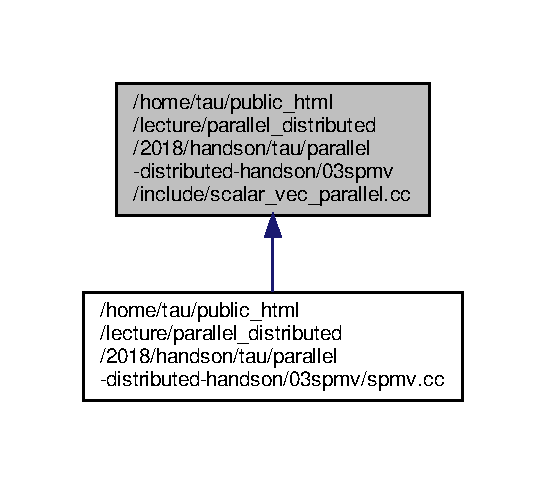
\includegraphics[width=237pt]{scalar__vec__parallel_8cc__dep__incl}
\end{center}
\end{figure}
\subsection*{Functions}
\begin{DoxyCompactItemize}
\item 
static int \hyperlink{scalar__vec__parallel_8cc_a26ccc7c1a9ee3268853441b1d0ce8f98}{scalar\+\_\+vec\+\_\+parallel} (\hyperlink{spmv_8cc_a11d147c64891830c9e79b3315b1b2e21}{real} k, \hyperlink{structvec__t}{vec\+\_\+t} v)
\begin{DoxyCompactList}\small\item\em k x v in parallel \end{DoxyCompactList}\end{DoxyCompactItemize}


\subsection{Detailed Description}
scalar x vector multiply with parallel for 



\subsection{Function Documentation}
\mbox{\Hypertarget{scalar__vec__parallel_8cc_a26ccc7c1a9ee3268853441b1d0ce8f98}\label{scalar__vec__parallel_8cc_a26ccc7c1a9ee3268853441b1d0ce8f98}} 
\index{scalar\+\_\+vec\+\_\+parallel.\+cc@{scalar\+\_\+vec\+\_\+parallel.\+cc}!scalar\+\_\+vec\+\_\+parallel@{scalar\+\_\+vec\+\_\+parallel}}
\index{scalar\+\_\+vec\+\_\+parallel@{scalar\+\_\+vec\+\_\+parallel}!scalar\+\_\+vec\+\_\+parallel.\+cc@{scalar\+\_\+vec\+\_\+parallel.\+cc}}
\subsubsection{\texorpdfstring{scalar\+\_\+vec\+\_\+parallel()}{scalar\_vec\_parallel()}}
{\footnotesize\ttfamily static int scalar\+\_\+vec\+\_\+parallel (\begin{DoxyParamCaption}\item[{\hyperlink{spmv_8cc_a11d147c64891830c9e79b3315b1b2e21}{real}}]{k,  }\item[{\hyperlink{structvec__t}{vec\+\_\+t}}]{v }\end{DoxyParamCaption})\hspace{0.3cm}{\ttfamily [static]}}



k x v in parallel 


\begin{DoxyParams}{Parameters}
{\em (k)} & a scalar \\
\hline
{\em (v)} & a vector \\
\hline
\end{DoxyParams}
\begin{DoxyReturn}{Returns}
1
\end{DoxyReturn}
multiply each element of v by k 
\hypertarget{scalar__vec__task_8cc}{}\section{/home/tau/public\+\_\+html/lecture/parallel\+\_\+distributed/2018/handson/tau/parallel-\/distributed-\/handson/03spmv/include/scalar\+\_\+vec\+\_\+task.cc File Reference}
\label{scalar__vec__task_8cc}\index{/home/tau/public\+\_\+html/lecture/parallel\+\_\+distributed/2018/handson/tau/parallel-\/distributed-\/handson/03spmv/include/scalar\+\_\+vec\+\_\+task.\+cc@{/home/tau/public\+\_\+html/lecture/parallel\+\_\+distributed/2018/handson/tau/parallel-\/distributed-\/handson/03spmv/include/scalar\+\_\+vec\+\_\+task.\+cc}}


scalar x vector multiply with tasks  


This graph shows which files directly or indirectly include this file\+:\nopagebreak
\begin{figure}[H]
\begin{center}
\leavevmode
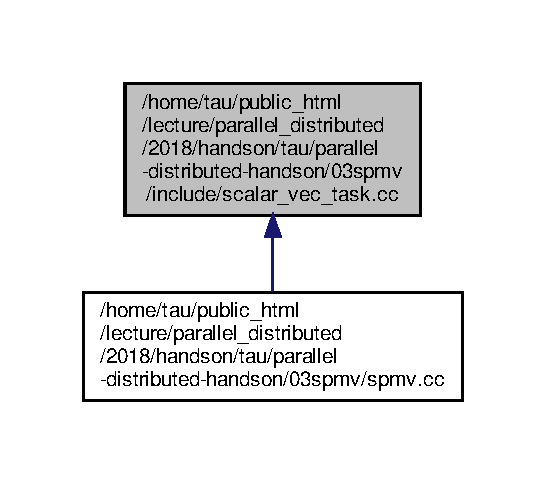
\includegraphics[width=262pt]{scalar__vec__task_8cc__dep__incl}
\end{center}
\end{figure}
\subsection*{Functions}
\begin{DoxyCompactItemize}
\item 
static int \hyperlink{scalar__vec__task_8cc_a7c173a211213a6c320853217b58e3a11}{scalar\+\_\+vec\+\_\+task} (\hyperlink{spmv_8cc_a11d147c64891830c9e79b3315b1b2e21}{real} k, \hyperlink{structvec__t}{vec\+\_\+t} v)
\begin{DoxyCompactList}\small\item\em k x v in parallel with tasks \end{DoxyCompactList}\end{DoxyCompactItemize}


\subsection{Detailed Description}
scalar x vector multiply with tasks 



\subsection{Function Documentation}
\mbox{\Hypertarget{scalar__vec__task_8cc_a7c173a211213a6c320853217b58e3a11}\label{scalar__vec__task_8cc_a7c173a211213a6c320853217b58e3a11}} 
\index{scalar\+\_\+vec\+\_\+task.\+cc@{scalar\+\_\+vec\+\_\+task.\+cc}!scalar\+\_\+vec\+\_\+task@{scalar\+\_\+vec\+\_\+task}}
\index{scalar\+\_\+vec\+\_\+task@{scalar\+\_\+vec\+\_\+task}!scalar\+\_\+vec\+\_\+task.\+cc@{scalar\+\_\+vec\+\_\+task.\+cc}}
\subsubsection{\texorpdfstring{scalar\+\_\+vec\+\_\+task()}{scalar\_vec\_task()}}
{\footnotesize\ttfamily static int scalar\+\_\+vec\+\_\+task (\begin{DoxyParamCaption}\item[{\hyperlink{spmv_8cc_a11d147c64891830c9e79b3315b1b2e21}{real}}]{k,  }\item[{\hyperlink{structvec__t}{vec\+\_\+t}}]{v }\end{DoxyParamCaption})\hspace{0.3cm}{\ttfamily [static]}}



k x v in parallel with tasks 


\begin{DoxyParams}{Parameters}
{\em (k)} & a scalar \\
\hline
{\em (v)} & a vector \\
\hline
\end{DoxyParams}
\begin{DoxyReturn}{Returns}
1
\end{DoxyReturn}
multiply each element of v by k 
\hypertarget{scalar__vec__udr_8cc}{}\section{/home/tau/public\+\_\+html/lecture/parallel\+\_\+distributed/2018/handson/tau/parallel-\/distributed-\/handson/03spmv/include/scalar\+\_\+vec\+\_\+udr.cc File Reference}
\label{scalar__vec__udr_8cc}\index{/home/tau/public\+\_\+html/lecture/parallel\+\_\+distributed/2018/handson/tau/parallel-\/distributed-\/handson/03spmv/include/scalar\+\_\+vec\+\_\+udr.\+cc@{/home/tau/public\+\_\+html/lecture/parallel\+\_\+distributed/2018/handson/tau/parallel-\/distributed-\/handson/03spmv/include/scalar\+\_\+vec\+\_\+udr.\+cc}}


scalar x vector multiply with parallel for + user-\/defined reductions  


This graph shows which files directly or indirectly include this file\+:\nopagebreak
\begin{figure}[H]
\begin{center}
\leavevmode
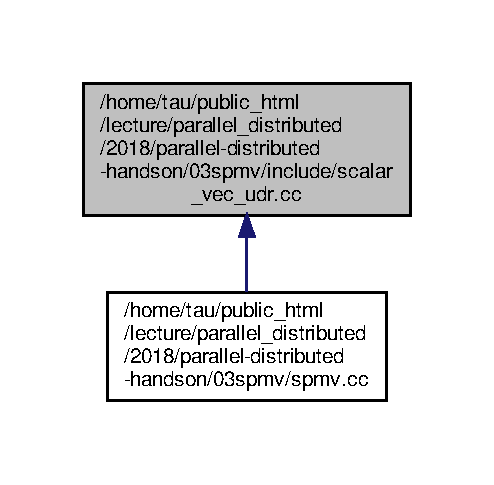
\includegraphics[width=262pt]{scalar__vec__udr_8cc__dep__incl}
\end{center}
\end{figure}
\subsection*{Functions}
\begin{DoxyCompactItemize}
\item 
static int \hyperlink{scalar__vec__udr_8cc_ad1461b5cf447013b133c040882692d3c}{scalar\+\_\+vec\+\_\+udr} (\hyperlink{spmv_8cc_a11d147c64891830c9e79b3315b1b2e21}{real} k, \hyperlink{structvec__t}{vec\+\_\+t} v)
\begin{DoxyCompactList}\small\item\em k x v in parallel with user-\/defined reductions \end{DoxyCompactList}\end{DoxyCompactItemize}


\subsection{Detailed Description}
scalar x vector multiply with parallel for + user-\/defined reductions 



\subsection{Function Documentation}
\mbox{\Hypertarget{scalar__vec__udr_8cc_ad1461b5cf447013b133c040882692d3c}\label{scalar__vec__udr_8cc_ad1461b5cf447013b133c040882692d3c}} 
\index{scalar\+\_\+vec\+\_\+udr.\+cc@{scalar\+\_\+vec\+\_\+udr.\+cc}!scalar\+\_\+vec\+\_\+udr@{scalar\+\_\+vec\+\_\+udr}}
\index{scalar\+\_\+vec\+\_\+udr@{scalar\+\_\+vec\+\_\+udr}!scalar\+\_\+vec\+\_\+udr.\+cc@{scalar\+\_\+vec\+\_\+udr.\+cc}}
\subsubsection{\texorpdfstring{scalar\+\_\+vec\+\_\+udr()}{scalar\_vec\_udr()}}
{\footnotesize\ttfamily static int scalar\+\_\+vec\+\_\+udr (\begin{DoxyParamCaption}\item[{\hyperlink{spmv_8cc_a11d147c64891830c9e79b3315b1b2e21}{real}}]{k,  }\item[{\hyperlink{structvec__t}{vec\+\_\+t}}]{v }\end{DoxyParamCaption})\hspace{0.3cm}{\ttfamily [static]}}



k x v in parallel with user-\/defined reductions 


\begin{DoxyParams}{Parameters}
{\em (k)} & a scalar \\
\hline
{\em (v)} & a vector \\
\hline
\end{DoxyParams}
\begin{DoxyReturn}{Returns}
1
\end{DoxyReturn}
multiply each element of v by k 
\hypertarget{spmv__coo__cuda_8cc}{}\section{/home/tau/public\+\_\+html/lecture/parallel\+\_\+distributed/2018/parallel-\/distributed-\/handson/03spmv/include/spmv\+\_\+coo\+\_\+cuda.cc File Reference}
\label{spmv__coo__cuda_8cc}\index{/home/tau/public\+\_\+html/lecture/parallel\+\_\+distributed/2018/parallel-\/distributed-\/handson/03spmv/include/spmv\+\_\+coo\+\_\+cuda.\+cc@{/home/tau/public\+\_\+html/lecture/parallel\+\_\+distributed/2018/parallel-\/distributed-\/handson/03spmv/include/spmv\+\_\+coo\+\_\+cuda.\+cc}}


y = A $\ast$ x for coo with cuda  


\subsection*{Functions}
\begin{DoxyCompactItemize}
\item 
\+\_\+\+\_\+global\+\_\+\+\_\+ void \hyperlink{spmv__coo__cuda_8cc_a38bf40a7fad355ba53f168a00c1f6b5a}{init\+\_\+const\+\_\+dev} (\hyperlink{structvec__t}{vec\+\_\+t} v, \hyperlink{spmv_8cc_a11d147c64891830c9e79b3315b1b2e21}{real} c)
\begin{DoxyCompactList}\small\item\em the device procedure to initialize all elements of v with a constant c \end{DoxyCompactList}\item 
\+\_\+\+\_\+global\+\_\+\+\_\+ void \hyperlink{spmv__coo__cuda_8cc_aa8b36d14695c5599ff6a2e724711101f}{spmv\+\_\+coo\+\_\+dev} (\hyperlink{structsparse__t}{sparse\+\_\+t} A, \hyperlink{structvec__t}{vec\+\_\+t} vx, \hyperlink{structvec__t}{vec\+\_\+t} vy)
\begin{DoxyCompactList}\small\item\em the device procedure to do spmv in coo format \end{DoxyCompactList}\item 
static int \hyperlink{spmv__coo__cuda_8cc_a0f69fc3347f24b8d0dff47851ba19aa4}{spmv\+\_\+coo\+\_\+cuda} (\hyperlink{structsparse__t}{sparse\+\_\+t} A, \hyperlink{structvec__t}{vec\+\_\+t} vx, \hyperlink{structvec__t}{vec\+\_\+t} vy)
\begin{DoxyCompactList}\small\item\em y = A $\ast$ x for coo with cuda \end{DoxyCompactList}\end{DoxyCompactItemize}


\subsection{Detailed Description}
y = A $\ast$ x for coo with cuda 



\subsection{Function Documentation}
\mbox{\Hypertarget{spmv__coo__cuda_8cc_a38bf40a7fad355ba53f168a00c1f6b5a}\label{spmv__coo__cuda_8cc_a38bf40a7fad355ba53f168a00c1f6b5a}} 
\index{spmv\+\_\+coo\+\_\+cuda.\+cc@{spmv\+\_\+coo\+\_\+cuda.\+cc}!init\+\_\+const\+\_\+dev@{init\+\_\+const\+\_\+dev}}
\index{init\+\_\+const\+\_\+dev@{init\+\_\+const\+\_\+dev}!spmv\+\_\+coo\+\_\+cuda.\+cc@{spmv\+\_\+coo\+\_\+cuda.\+cc}}
\subsubsection{\texorpdfstring{init\+\_\+const\+\_\+dev()}{init\_const\_dev()}}
{\footnotesize\ttfamily \+\_\+\+\_\+global\+\_\+\+\_\+ void init\+\_\+const\+\_\+dev (\begin{DoxyParamCaption}\item[{\hyperlink{structvec__t}{vec\+\_\+t}}]{v,  }\item[{\hyperlink{spmv_8cc_a11d147c64891830c9e79b3315b1b2e21}{real}}]{c }\end{DoxyParamCaption})}



the device procedure to initialize all elements of v with a constant c 


\begin{DoxyParams}{Parameters}
{\em (v)} & a vector \\
\hline
{\em (c)} & the value to initialize all v\textquotesingle{}s elements with \\
\hline
\end{DoxyParams}
\mbox{\Hypertarget{spmv__coo__cuda_8cc_a0f69fc3347f24b8d0dff47851ba19aa4}\label{spmv__coo__cuda_8cc_a0f69fc3347f24b8d0dff47851ba19aa4}} 
\index{spmv\+\_\+coo\+\_\+cuda.\+cc@{spmv\+\_\+coo\+\_\+cuda.\+cc}!spmv\+\_\+coo\+\_\+cuda@{spmv\+\_\+coo\+\_\+cuda}}
\index{spmv\+\_\+coo\+\_\+cuda@{spmv\+\_\+coo\+\_\+cuda}!spmv\+\_\+coo\+\_\+cuda.\+cc@{spmv\+\_\+coo\+\_\+cuda.\+cc}}
\subsubsection{\texorpdfstring{spmv\+\_\+coo\+\_\+cuda()}{spmv\_coo\_cuda()}}
{\footnotesize\ttfamily static int spmv\+\_\+coo\+\_\+cuda (\begin{DoxyParamCaption}\item[{\hyperlink{structsparse__t}{sparse\+\_\+t}}]{A,  }\item[{\hyperlink{structvec__t}{vec\+\_\+t}}]{vx,  }\item[{\hyperlink{structvec__t}{vec\+\_\+t}}]{vy }\end{DoxyParamCaption})\hspace{0.3cm}{\ttfamily [static]}}



y = A $\ast$ x for coo with cuda 


\begin{DoxyParams}{Parameters}
{\em (\+A)} & a sparse matrix in coo format \\
\hline
{\em (vx)} & a vector \\
\hline
{\em (vy)} & a vector \\
\hline
\end{DoxyParams}
\begin{DoxyReturn}{Returns}
1 if succeed, 0 if failed 
\end{DoxyReturn}
\mbox{\Hypertarget{spmv__coo__cuda_8cc_aa8b36d14695c5599ff6a2e724711101f}\label{spmv__coo__cuda_8cc_aa8b36d14695c5599ff6a2e724711101f}} 
\index{spmv\+\_\+coo\+\_\+cuda.\+cc@{spmv\+\_\+coo\+\_\+cuda.\+cc}!spmv\+\_\+coo\+\_\+dev@{spmv\+\_\+coo\+\_\+dev}}
\index{spmv\+\_\+coo\+\_\+dev@{spmv\+\_\+coo\+\_\+dev}!spmv\+\_\+coo\+\_\+cuda.\+cc@{spmv\+\_\+coo\+\_\+cuda.\+cc}}
\subsubsection{\texorpdfstring{spmv\+\_\+coo\+\_\+dev()}{spmv\_coo\_dev()}}
{\footnotesize\ttfamily \+\_\+\+\_\+global\+\_\+\+\_\+ void spmv\+\_\+coo\+\_\+dev (\begin{DoxyParamCaption}\item[{\hyperlink{structsparse__t}{sparse\+\_\+t}}]{A,  }\item[{\hyperlink{structvec__t}{vec\+\_\+t}}]{vx,  }\item[{\hyperlink{structvec__t}{vec\+\_\+t}}]{vy }\end{DoxyParamCaption})}



the device procedure to do spmv in coo format 


\begin{DoxyParams}{Parameters}
{\em (\+A)} & a sparse matrix \\
\hline
{\em (vx)} & a vector \\
\hline
{\em (vy)} & a vector\\
\hline
\end{DoxyParams}
assume A, vx, vy must have their elems\+\_\+dev already set. 
\hypertarget{spmv__coo__parallel_8cc}{}\section{/home/tau/public\+\_\+html/lecture/parallel\+\_\+distributed/2018/parallel-\/distributed-\/handson/03spmv/include/spmv\+\_\+coo\+\_\+parallel.cc File Reference}
\label{spmv__coo__parallel_8cc}\index{/home/tau/public\+\_\+html/lecture/parallel\+\_\+distributed/2018/parallel-\/distributed-\/handson/03spmv/include/spmv\+\_\+coo\+\_\+parallel.\+cc@{/home/tau/public\+\_\+html/lecture/parallel\+\_\+distributed/2018/parallel-\/distributed-\/handson/03spmv/include/spmv\+\_\+coo\+\_\+parallel.\+cc}}


y = A $\ast$ x for coo with parallel for  


This graph shows which files directly or indirectly include this file\+:\nopagebreak
\begin{figure}[H]
\begin{center}
\leavevmode
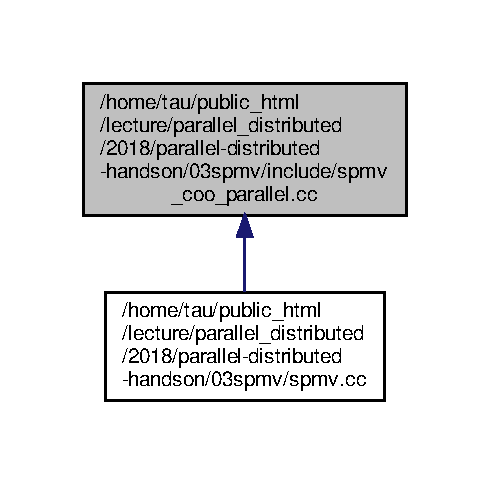
\includegraphics[width=235pt]{spmv__coo__parallel_8cc__dep__incl}
\end{center}
\end{figure}
\subsection*{Functions}
\begin{DoxyCompactItemize}
\item 
static int \hyperlink{spmv__coo__parallel_8cc_ada3d431757871be30e0fe48b89a33973}{spmv\+\_\+coo\+\_\+parallel} (\hyperlink{structsparse__t}{sparse\+\_\+t} A, \hyperlink{structvec__t}{vec\+\_\+t} vx, \hyperlink{structvec__t}{vec\+\_\+t} vy)
\begin{DoxyCompactList}\small\item\em y = A $\ast$ x for coo with parallel for \end{DoxyCompactList}\end{DoxyCompactItemize}


\subsection{Detailed Description}
y = A $\ast$ x for coo with parallel for 



\subsection{Function Documentation}
\mbox{\Hypertarget{spmv__coo__parallel_8cc_ada3d431757871be30e0fe48b89a33973}\label{spmv__coo__parallel_8cc_ada3d431757871be30e0fe48b89a33973}} 
\index{spmv\+\_\+coo\+\_\+parallel.\+cc@{spmv\+\_\+coo\+\_\+parallel.\+cc}!spmv\+\_\+coo\+\_\+parallel@{spmv\+\_\+coo\+\_\+parallel}}
\index{spmv\+\_\+coo\+\_\+parallel@{spmv\+\_\+coo\+\_\+parallel}!spmv\+\_\+coo\+\_\+parallel.\+cc@{spmv\+\_\+coo\+\_\+parallel.\+cc}}
\subsubsection{\texorpdfstring{spmv\+\_\+coo\+\_\+parallel()}{spmv\_coo\_parallel()}}
{\footnotesize\ttfamily static int spmv\+\_\+coo\+\_\+parallel (\begin{DoxyParamCaption}\item[{\hyperlink{structsparse__t}{sparse\+\_\+t}}]{A,  }\item[{\hyperlink{structvec__t}{vec\+\_\+t}}]{vx,  }\item[{\hyperlink{structvec__t}{vec\+\_\+t}}]{vy }\end{DoxyParamCaption})\hspace{0.3cm}{\ttfamily [static]}}



y = A $\ast$ x for coo with parallel for 


\begin{DoxyParams}{Parameters}
{\em (\+A)} & a sparse matrix \\
\hline
{\em (vx)} & a vector \\
\hline
{\em (vy)} & a vector \\
\hline
\end{DoxyParams}
\begin{DoxyReturn}{Returns}
1 if succeed, 0 if failed 
\end{DoxyReturn}

\hypertarget{spmv__coo__sorted__cuda_8cc}{}\section{/home/tau/public\+\_\+html/lecture/parallel\+\_\+distributed/2018/parallel-\/distributed-\/handson/03spmv/include/spmv\+\_\+coo\+\_\+sorted\+\_\+cuda.cc File Reference}
\label{spmv__coo__sorted__cuda_8cc}\index{/home/tau/public\+\_\+html/lecture/parallel\+\_\+distributed/2018/parallel-\/distributed-\/handson/03spmv/include/spmv\+\_\+coo\+\_\+sorted\+\_\+cuda.\+cc@{/home/tau/public\+\_\+html/lecture/parallel\+\_\+distributed/2018/parallel-\/distributed-\/handson/03spmv/include/spmv\+\_\+coo\+\_\+sorted\+\_\+cuda.\+cc}}


y = A $\ast$ x for coo\+\_\+sorted with cuda  


\subsection*{Functions}
\begin{DoxyCompactItemize}
\item 
static int \hyperlink{spmv__coo__sorted__cuda_8cc_a0c7f09dff7ec7a603acd26a19a44450d}{spmv\+\_\+coo\+\_\+sorted\+\_\+cuda} (\hyperlink{structsparse__t}{sparse\+\_\+t} A, \hyperlink{structvec__t}{vec\+\_\+t} vx, \hyperlink{structvec__t}{vec\+\_\+t} vy)
\begin{DoxyCompactList}\small\item\em y = A $\ast$ x for coo\+\_\+sorted with cuda \end{DoxyCompactList}\end{DoxyCompactItemize}


\subsection{Detailed Description}
y = A $\ast$ x for coo\+\_\+sorted with cuda 



\subsection{Function Documentation}
\mbox{\Hypertarget{spmv__coo__sorted__cuda_8cc_a0c7f09dff7ec7a603acd26a19a44450d}\label{spmv__coo__sorted__cuda_8cc_a0c7f09dff7ec7a603acd26a19a44450d}} 
\index{spmv\+\_\+coo\+\_\+sorted\+\_\+cuda.\+cc@{spmv\+\_\+coo\+\_\+sorted\+\_\+cuda.\+cc}!spmv\+\_\+coo\+\_\+sorted\+\_\+cuda@{spmv\+\_\+coo\+\_\+sorted\+\_\+cuda}}
\index{spmv\+\_\+coo\+\_\+sorted\+\_\+cuda@{spmv\+\_\+coo\+\_\+sorted\+\_\+cuda}!spmv\+\_\+coo\+\_\+sorted\+\_\+cuda.\+cc@{spmv\+\_\+coo\+\_\+sorted\+\_\+cuda.\+cc}}
\subsubsection{\texorpdfstring{spmv\+\_\+coo\+\_\+sorted\+\_\+cuda()}{spmv\_coo\_sorted\_cuda()}}
{\footnotesize\ttfamily static int spmv\+\_\+coo\+\_\+sorted\+\_\+cuda (\begin{DoxyParamCaption}\item[{\hyperlink{structsparse__t}{sparse\+\_\+t}}]{A,  }\item[{\hyperlink{structvec__t}{vec\+\_\+t}}]{vx,  }\item[{\hyperlink{structvec__t}{vec\+\_\+t}}]{vy }\end{DoxyParamCaption})\hspace{0.3cm}{\ttfamily [static]}}



y = A $\ast$ x for coo\+\_\+sorted with cuda 


\begin{DoxyParams}{Parameters}
{\em (\+A)} & a sparse matrix \\
\hline
{\em (vx)} & a vector \\
\hline
{\em (vy)} & a vector \\
\hline
\end{DoxyParams}
\begin{DoxyReturn}{Returns}
1 if succeed, 0 if failed 
\end{DoxyReturn}

\hypertarget{spmv__coo__sorted__parallel_8cc}{}\section{/home/tau/public\+\_\+html/lecture/parallel\+\_\+distributed/2018/parallel-\/distributed-\/handson/03spmv/include/spmv\+\_\+coo\+\_\+sorted\+\_\+parallel.cc File Reference}
\label{spmv__coo__sorted__parallel_8cc}\index{/home/tau/public\+\_\+html/lecture/parallel\+\_\+distributed/2018/parallel-\/distributed-\/handson/03spmv/include/spmv\+\_\+coo\+\_\+sorted\+\_\+parallel.\+cc@{/home/tau/public\+\_\+html/lecture/parallel\+\_\+distributed/2018/parallel-\/distributed-\/handson/03spmv/include/spmv\+\_\+coo\+\_\+sorted\+\_\+parallel.\+cc}}


y = A $\ast$ x for coo\+\_\+sorted with parallel for  


This graph shows which files directly or indirectly include this file\+:\nopagebreak
\begin{figure}[H]
\begin{center}
\leavevmode
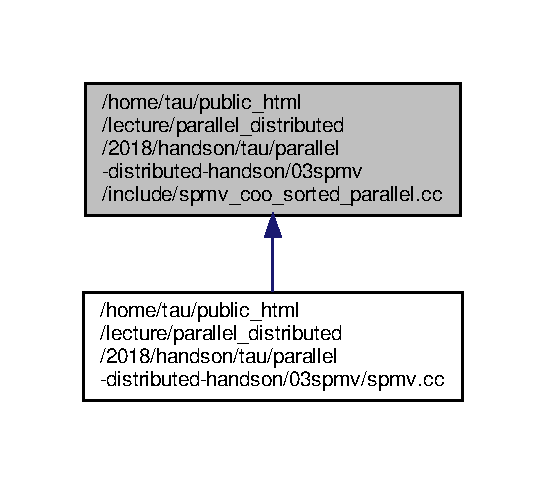
\includegraphics[width=235pt]{spmv__coo__sorted__parallel_8cc__dep__incl}
\end{center}
\end{figure}
\subsection*{Functions}
\begin{DoxyCompactItemize}
\item 
static int \hyperlink{spmv__coo__sorted__parallel_8cc_a288772ff3dade2ab26450de5349b2d10}{spmv\+\_\+coo\+\_\+sorted\+\_\+parallel} (\hyperlink{structsparse__t}{sparse\+\_\+t} A, \hyperlink{structvec__t}{vec\+\_\+t} vx, \hyperlink{structvec__t}{vec\+\_\+t} vy)
\begin{DoxyCompactList}\small\item\em y = A $\ast$ x for coo\+\_\+sorted with parallel for \end{DoxyCompactList}\end{DoxyCompactItemize}


\subsection{Detailed Description}
y = A $\ast$ x for coo\+\_\+sorted with parallel for 



\subsection{Function Documentation}
\mbox{\Hypertarget{spmv__coo__sorted__parallel_8cc_a288772ff3dade2ab26450de5349b2d10}\label{spmv__coo__sorted__parallel_8cc_a288772ff3dade2ab26450de5349b2d10}} 
\index{spmv\+\_\+coo\+\_\+sorted\+\_\+parallel.\+cc@{spmv\+\_\+coo\+\_\+sorted\+\_\+parallel.\+cc}!spmv\+\_\+coo\+\_\+sorted\+\_\+parallel@{spmv\+\_\+coo\+\_\+sorted\+\_\+parallel}}
\index{spmv\+\_\+coo\+\_\+sorted\+\_\+parallel@{spmv\+\_\+coo\+\_\+sorted\+\_\+parallel}!spmv\+\_\+coo\+\_\+sorted\+\_\+parallel.\+cc@{spmv\+\_\+coo\+\_\+sorted\+\_\+parallel.\+cc}}
\subsubsection{\texorpdfstring{spmv\+\_\+coo\+\_\+sorted\+\_\+parallel()}{spmv\_coo\_sorted\_parallel()}}
{\footnotesize\ttfamily static int spmv\+\_\+coo\+\_\+sorted\+\_\+parallel (\begin{DoxyParamCaption}\item[{\hyperlink{structsparse__t}{sparse\+\_\+t}}]{A,  }\item[{\hyperlink{structvec__t}{vec\+\_\+t}}]{vx,  }\item[{\hyperlink{structvec__t}{vec\+\_\+t}}]{vy }\end{DoxyParamCaption})\hspace{0.3cm}{\ttfamily [static]}}



y = A $\ast$ x for coo\+\_\+sorted with parallel for 


\begin{DoxyParams}{Parameters}
{\em (\+A)} & a sparse matrix \\
\hline
{\em (vx)} & a vector \\
\hline
{\em (vy)} & a vector \\
\hline
\end{DoxyParams}
\begin{DoxyReturn}{Returns}
1 if succeed, 0 if failed 
\end{DoxyReturn}

\hypertarget{spmv__coo__sorted__task_8cc}{}\section{/home/tau/public\+\_\+html/lecture/parallel\+\_\+distributed/2018/handson/tau/parallel-\/distributed-\/handson/03spmv/include/spmv\+\_\+coo\+\_\+sorted\+\_\+task.cc File Reference}
\label{spmv__coo__sorted__task_8cc}\index{/home/tau/public\+\_\+html/lecture/parallel\+\_\+distributed/2018/handson/tau/parallel-\/distributed-\/handson/03spmv/include/spmv\+\_\+coo\+\_\+sorted\+\_\+task.\+cc@{/home/tau/public\+\_\+html/lecture/parallel\+\_\+distributed/2018/handson/tau/parallel-\/distributed-\/handson/03spmv/include/spmv\+\_\+coo\+\_\+sorted\+\_\+task.\+cc}}


y = A $\ast$ x with tasks for coo\+\_\+sorted  


This graph shows which files directly or indirectly include this file\+:\nopagebreak
\begin{figure}[H]
\begin{center}
\leavevmode
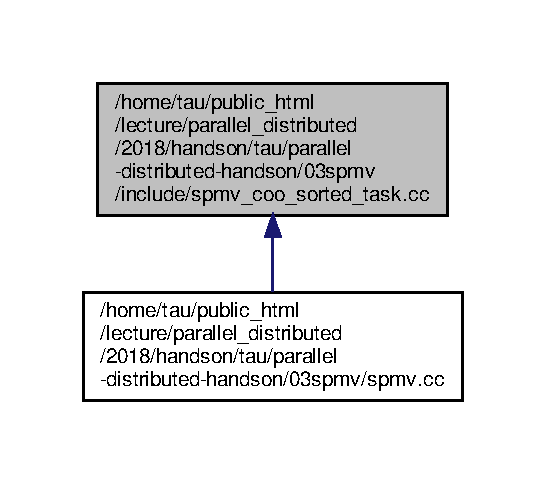
\includegraphics[width=262pt]{spmv__coo__sorted__task_8cc__dep__incl}
\end{center}
\end{figure}
\subsection*{Functions}
\begin{DoxyCompactItemize}
\item 
static int \hyperlink{spmv__coo__sorted__task_8cc_a54003161e4ed3de194a75c43ae8338d4}{spmv\+\_\+coo\+\_\+sorted\+\_\+task} (\hyperlink{structsparse__t}{sparse\+\_\+t} A, \hyperlink{structvec__t}{vec\+\_\+t} vx, \hyperlink{structvec__t}{vec\+\_\+t} vy)
\begin{DoxyCompactList}\small\item\em y = A $\ast$ x with tasks for coo\+\_\+sorted \end{DoxyCompactList}\end{DoxyCompactItemize}


\subsection{Detailed Description}
y = A $\ast$ x with tasks for coo\+\_\+sorted 



\subsection{Function Documentation}
\mbox{\Hypertarget{spmv__coo__sorted__task_8cc_a54003161e4ed3de194a75c43ae8338d4}\label{spmv__coo__sorted__task_8cc_a54003161e4ed3de194a75c43ae8338d4}} 
\index{spmv\+\_\+coo\+\_\+sorted\+\_\+task.\+cc@{spmv\+\_\+coo\+\_\+sorted\+\_\+task.\+cc}!spmv\+\_\+coo\+\_\+sorted\+\_\+task@{spmv\+\_\+coo\+\_\+sorted\+\_\+task}}
\index{spmv\+\_\+coo\+\_\+sorted\+\_\+task@{spmv\+\_\+coo\+\_\+sorted\+\_\+task}!spmv\+\_\+coo\+\_\+sorted\+\_\+task.\+cc@{spmv\+\_\+coo\+\_\+sorted\+\_\+task.\+cc}}
\subsubsection{\texorpdfstring{spmv\+\_\+coo\+\_\+sorted\+\_\+task()}{spmv\_coo\_sorted\_task()}}
{\footnotesize\ttfamily static int spmv\+\_\+coo\+\_\+sorted\+\_\+task (\begin{DoxyParamCaption}\item[{\hyperlink{structsparse__t}{sparse\+\_\+t}}]{A,  }\item[{\hyperlink{structvec__t}{vec\+\_\+t}}]{vx,  }\item[{\hyperlink{structvec__t}{vec\+\_\+t}}]{vy }\end{DoxyParamCaption})\hspace{0.3cm}{\ttfamily [static]}}



y = A $\ast$ x with tasks for coo\+\_\+sorted 


\begin{DoxyParams}{Parameters}
{\em (\+A)} & a sparse matrix \\
\hline
{\em (vx)} & a vector \\
\hline
{\em (vy)} & a vector \\
\hline
\end{DoxyParams}
\begin{DoxyReturn}{Returns}
1 if succeed, 0 if failed 
\end{DoxyReturn}

\hypertarget{spmv__coo__sorted__udr_8cc}{}\section{/home/tau/public\+\_\+html/lecture/parallel\+\_\+distributed/2018/handson/tau/parallel-\/distributed-\/handson/03spmv/include/spmv\+\_\+coo\+\_\+sorted\+\_\+udr.cc File Reference}
\label{spmv__coo__sorted__udr_8cc}\index{/home/tau/public\+\_\+html/lecture/parallel\+\_\+distributed/2018/handson/tau/parallel-\/distributed-\/handson/03spmv/include/spmv\+\_\+coo\+\_\+sorted\+\_\+udr.\+cc@{/home/tau/public\+\_\+html/lecture/parallel\+\_\+distributed/2018/handson/tau/parallel-\/distributed-\/handson/03spmv/include/spmv\+\_\+coo\+\_\+sorted\+\_\+udr.\+cc}}


y = A $\ast$ x for coo\+\_\+sorted with parallel for + user-\/defined reductions  


This graph shows which files directly or indirectly include this file\+:\nopagebreak
\begin{figure}[H]
\begin{center}
\leavevmode
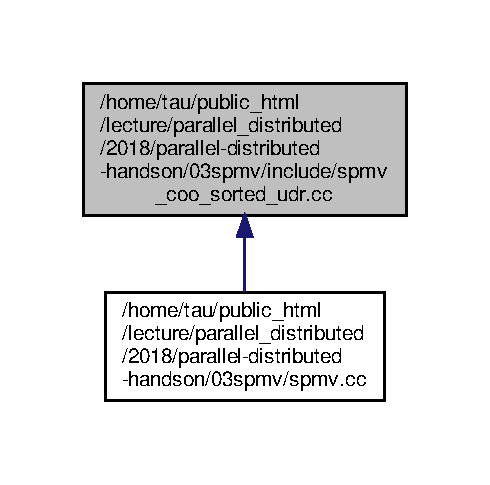
\includegraphics[width=262pt]{spmv__coo__sorted__udr_8cc__dep__incl}
\end{center}
\end{figure}
\subsection*{Functions}
\begin{DoxyCompactItemize}
\item 
static int \hyperlink{spmv__coo__sorted__udr_8cc_acd8cf86cbdc5f244e2e28364e73e4ce9}{spmv\+\_\+coo\+\_\+sorted\+\_\+udr} (\hyperlink{structsparse__t}{sparse\+\_\+t} A, \hyperlink{structvec__t}{vec\+\_\+t} vx, \hyperlink{structvec__t}{vec\+\_\+t} vy)
\begin{DoxyCompactList}\small\item\em y = A $\ast$ x for coo\+\_\+sorted with parallel for + user-\/defined reductions \end{DoxyCompactList}\end{DoxyCompactItemize}


\subsection{Detailed Description}
y = A $\ast$ x for coo\+\_\+sorted with parallel for + user-\/defined reductions 



\subsection{Function Documentation}
\mbox{\Hypertarget{spmv__coo__sorted__udr_8cc_acd8cf86cbdc5f244e2e28364e73e4ce9}\label{spmv__coo__sorted__udr_8cc_acd8cf86cbdc5f244e2e28364e73e4ce9}} 
\index{spmv\+\_\+coo\+\_\+sorted\+\_\+udr.\+cc@{spmv\+\_\+coo\+\_\+sorted\+\_\+udr.\+cc}!spmv\+\_\+coo\+\_\+sorted\+\_\+udr@{spmv\+\_\+coo\+\_\+sorted\+\_\+udr}}
\index{spmv\+\_\+coo\+\_\+sorted\+\_\+udr@{spmv\+\_\+coo\+\_\+sorted\+\_\+udr}!spmv\+\_\+coo\+\_\+sorted\+\_\+udr.\+cc@{spmv\+\_\+coo\+\_\+sorted\+\_\+udr.\+cc}}
\subsubsection{\texorpdfstring{spmv\+\_\+coo\+\_\+sorted\+\_\+udr()}{spmv\_coo\_sorted\_udr()}}
{\footnotesize\ttfamily static int spmv\+\_\+coo\+\_\+sorted\+\_\+udr (\begin{DoxyParamCaption}\item[{\hyperlink{structsparse__t}{sparse\+\_\+t}}]{A,  }\item[{\hyperlink{structvec__t}{vec\+\_\+t}}]{vx,  }\item[{\hyperlink{structvec__t}{vec\+\_\+t}}]{vy }\end{DoxyParamCaption})\hspace{0.3cm}{\ttfamily [static]}}



y = A $\ast$ x for coo\+\_\+sorted with parallel for + user-\/defined reductions 


\begin{DoxyParams}{Parameters}
{\em (\+A)} & a sparse matrix \\
\hline
{\em (vx)} & a vector \\
\hline
{\em (vy)} & a vector \\
\hline
\end{DoxyParams}
\begin{DoxyReturn}{Returns}
1 if succeed, 0 if failed 
\end{DoxyReturn}

\hypertarget{spmv__coo__task_8cc}{}\section{/home/tau/public\+\_\+html/lecture/parallel\+\_\+distributed/2018/parallel-\/distributed-\/handson/03spmv/include/spmv\+\_\+coo\+\_\+task.cc File Reference}
\label{spmv__coo__task_8cc}\index{/home/tau/public\+\_\+html/lecture/parallel\+\_\+distributed/2018/parallel-\/distributed-\/handson/03spmv/include/spmv\+\_\+coo\+\_\+task.\+cc@{/home/tau/public\+\_\+html/lecture/parallel\+\_\+distributed/2018/parallel-\/distributed-\/handson/03spmv/include/spmv\+\_\+coo\+\_\+task.\+cc}}


y = A $\ast$ x for coo with tasks  


This graph shows which files directly or indirectly include this file\+:\nopagebreak
\begin{figure}[H]
\begin{center}
\leavevmode
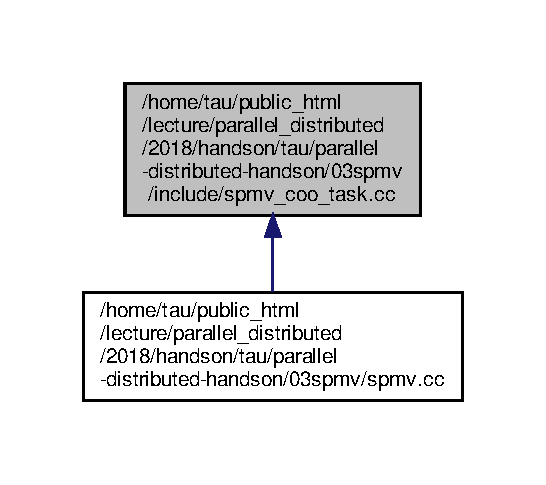
\includegraphics[width=235pt]{spmv__coo__task_8cc__dep__incl}
\end{center}
\end{figure}
\subsection*{Functions}
\begin{DoxyCompactItemize}
\item 
static int \hyperlink{spmv__coo__task_8cc_a0a02ba419ed338501ccf990bb7019429}{spmv\+\_\+coo\+\_\+task} (\hyperlink{structsparse__t}{sparse\+\_\+t} A, \hyperlink{structvec__t}{vec\+\_\+t} vx, \hyperlink{structvec__t}{vec\+\_\+t} vy)
\begin{DoxyCompactList}\small\item\em y = A $\ast$ x for coo with tasks \end{DoxyCompactList}\end{DoxyCompactItemize}


\subsection{Detailed Description}
y = A $\ast$ x for coo with tasks 



\subsection{Function Documentation}
\mbox{\Hypertarget{spmv__coo__task_8cc_a0a02ba419ed338501ccf990bb7019429}\label{spmv__coo__task_8cc_a0a02ba419ed338501ccf990bb7019429}} 
\index{spmv\+\_\+coo\+\_\+task.\+cc@{spmv\+\_\+coo\+\_\+task.\+cc}!spmv\+\_\+coo\+\_\+task@{spmv\+\_\+coo\+\_\+task}}
\index{spmv\+\_\+coo\+\_\+task@{spmv\+\_\+coo\+\_\+task}!spmv\+\_\+coo\+\_\+task.\+cc@{spmv\+\_\+coo\+\_\+task.\+cc}}
\subsubsection{\texorpdfstring{spmv\+\_\+coo\+\_\+task()}{spmv\_coo\_task()}}
{\footnotesize\ttfamily static int spmv\+\_\+coo\+\_\+task (\begin{DoxyParamCaption}\item[{\hyperlink{structsparse__t}{sparse\+\_\+t}}]{A,  }\item[{\hyperlink{structvec__t}{vec\+\_\+t}}]{vx,  }\item[{\hyperlink{structvec__t}{vec\+\_\+t}}]{vy }\end{DoxyParamCaption})\hspace{0.3cm}{\ttfamily [static]}}



y = A $\ast$ x for coo with tasks 


\begin{DoxyParams}{Parameters}
{\em (\+A)} & a sparse matrix \\
\hline
{\em (vx)} & a vector \\
\hline
{\em (vy)} & a vector \\
\hline
\end{DoxyParams}
\begin{DoxyReturn}{Returns}
1 if succeed, 0 if failed 
\end{DoxyReturn}

\hypertarget{spmv__coo__udr_8cc}{}\section{/home/tau/public\+\_\+html/lecture/parallel\+\_\+distributed/2018/parallel-\/distributed-\/handson/03spmv/include/spmv\+\_\+coo\+\_\+udr.cc File Reference}
\label{spmv__coo__udr_8cc}\index{/home/tau/public\+\_\+html/lecture/parallel\+\_\+distributed/2018/parallel-\/distributed-\/handson/03spmv/include/spmv\+\_\+coo\+\_\+udr.\+cc@{/home/tau/public\+\_\+html/lecture/parallel\+\_\+distributed/2018/parallel-\/distributed-\/handson/03spmv/include/spmv\+\_\+coo\+\_\+udr.\+cc}}


y = A $\ast$ x for coo with parallel for + user-\/defined reductions  


This graph shows which files directly or indirectly include this file\+:\nopagebreak
\begin{figure}[H]
\begin{center}
\leavevmode
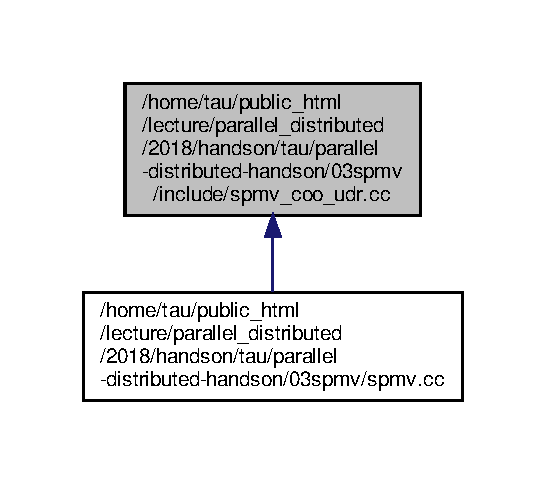
\includegraphics[width=235pt]{spmv__coo__udr_8cc__dep__incl}
\end{center}
\end{figure}
\subsection*{Functions}
\begin{DoxyCompactItemize}
\item 
static int \hyperlink{spmv__coo__udr_8cc_ac0d55e45d8bdc6031dc8d948da81b12c}{spmv\+\_\+coo\+\_\+udr} (\hyperlink{structsparse__t}{sparse\+\_\+t} A, \hyperlink{structvec__t}{vec\+\_\+t} vx, \hyperlink{structvec__t}{vec\+\_\+t} vy)
\begin{DoxyCompactList}\small\item\em y = A $\ast$ x for coo with parallel for + user-\/defined reductions \end{DoxyCompactList}\end{DoxyCompactItemize}


\subsection{Detailed Description}
y = A $\ast$ x for coo with parallel for + user-\/defined reductions 



\subsection{Function Documentation}
\mbox{\Hypertarget{spmv__coo__udr_8cc_ac0d55e45d8bdc6031dc8d948da81b12c}\label{spmv__coo__udr_8cc_ac0d55e45d8bdc6031dc8d948da81b12c}} 
\index{spmv\+\_\+coo\+\_\+udr.\+cc@{spmv\+\_\+coo\+\_\+udr.\+cc}!spmv\+\_\+coo\+\_\+udr@{spmv\+\_\+coo\+\_\+udr}}
\index{spmv\+\_\+coo\+\_\+udr@{spmv\+\_\+coo\+\_\+udr}!spmv\+\_\+coo\+\_\+udr.\+cc@{spmv\+\_\+coo\+\_\+udr.\+cc}}
\subsubsection{\texorpdfstring{spmv\+\_\+coo\+\_\+udr()}{spmv\_coo\_udr()}}
{\footnotesize\ttfamily static int spmv\+\_\+coo\+\_\+udr (\begin{DoxyParamCaption}\item[{\hyperlink{structsparse__t}{sparse\+\_\+t}}]{A,  }\item[{\hyperlink{structvec__t}{vec\+\_\+t}}]{vx,  }\item[{\hyperlink{structvec__t}{vec\+\_\+t}}]{vy }\end{DoxyParamCaption})\hspace{0.3cm}{\ttfamily [static]}}



y = A $\ast$ x for coo with parallel for + user-\/defined reductions 


\begin{DoxyParams}{Parameters}
{\em (\+A)} & a sparse matrix \\
\hline
{\em (vx)} & a vector \\
\hline
{\em (vy)} & a vector \\
\hline
\end{DoxyParams}
\begin{DoxyReturn}{Returns}
1 if succeed, 0 if failed 
\end{DoxyReturn}

\hypertarget{spmv__csr__cuda_8cc}{}\section{/home/tau/public\+\_\+html/lecture/parallel\+\_\+distributed/2018/handson/tau/parallel-\/distributed-\/handson/03spmv/include/spmv\+\_\+csr\+\_\+cuda.cc File Reference}
\label{spmv__csr__cuda_8cc}\index{/home/tau/public\+\_\+html/lecture/parallel\+\_\+distributed/2018/handson/tau/parallel-\/distributed-\/handson/03spmv/include/spmv\+\_\+csr\+\_\+cuda.\+cc@{/home/tau/public\+\_\+html/lecture/parallel\+\_\+distributed/2018/handson/tau/parallel-\/distributed-\/handson/03spmv/include/spmv\+\_\+csr\+\_\+cuda.\+cc}}


y = A $\ast$ x for csr with cuda  


\subsection*{Functions}
\begin{DoxyCompactItemize}
\item 
static int \hyperlink{spmv__csr__cuda_8cc_abfe0e8ff9d93cc6da3bbe47f3f9b8ea9}{spmv\+\_\+csr\+\_\+cuda} (\hyperlink{structsparse__t}{sparse\+\_\+t} A, \hyperlink{structvec__t}{vec\+\_\+t} vx, \hyperlink{structvec__t}{vec\+\_\+t} vy)
\begin{DoxyCompactList}\small\item\em y = A $\ast$ x for csr with cuda \end{DoxyCompactList}\end{DoxyCompactItemize}


\subsection{Detailed Description}
y = A $\ast$ x for csr with cuda 



\subsection{Function Documentation}
\mbox{\Hypertarget{spmv__csr__cuda_8cc_abfe0e8ff9d93cc6da3bbe47f3f9b8ea9}\label{spmv__csr__cuda_8cc_abfe0e8ff9d93cc6da3bbe47f3f9b8ea9}} 
\index{spmv\+\_\+csr\+\_\+cuda.\+cc@{spmv\+\_\+csr\+\_\+cuda.\+cc}!spmv\+\_\+csr\+\_\+cuda@{spmv\+\_\+csr\+\_\+cuda}}
\index{spmv\+\_\+csr\+\_\+cuda@{spmv\+\_\+csr\+\_\+cuda}!spmv\+\_\+csr\+\_\+cuda.\+cc@{spmv\+\_\+csr\+\_\+cuda.\+cc}}
\subsubsection{\texorpdfstring{spmv\+\_\+csr\+\_\+cuda()}{spmv\_csr\_cuda()}}
{\footnotesize\ttfamily static int spmv\+\_\+csr\+\_\+cuda (\begin{DoxyParamCaption}\item[{\hyperlink{structsparse__t}{sparse\+\_\+t}}]{A,  }\item[{\hyperlink{structvec__t}{vec\+\_\+t}}]{vx,  }\item[{\hyperlink{structvec__t}{vec\+\_\+t}}]{vy }\end{DoxyParamCaption})\hspace{0.3cm}{\ttfamily [static]}}



y = A $\ast$ x for csr with cuda 


\begin{DoxyParams}{Parameters}
{\em (\+A)} & a sparse matrix \\
\hline
{\em (vx)} & a vector \\
\hline
{\em (vy)} & a vector \\
\hline
\end{DoxyParams}
\begin{DoxyReturn}{Returns}
1 if succeed, 0 if failed 
\end{DoxyReturn}

\hypertarget{spmv__csr__parallel_8cc}{}\section{/home/tau/public\+\_\+html/lecture/parallel\+\_\+distributed/2018/parallel-\/distributed-\/handson/03spmv/include/spmv\+\_\+csr\+\_\+parallel.cc File Reference}
\label{spmv__csr__parallel_8cc}\index{/home/tau/public\+\_\+html/lecture/parallel\+\_\+distributed/2018/parallel-\/distributed-\/handson/03spmv/include/spmv\+\_\+csr\+\_\+parallel.\+cc@{/home/tau/public\+\_\+html/lecture/parallel\+\_\+distributed/2018/parallel-\/distributed-\/handson/03spmv/include/spmv\+\_\+csr\+\_\+parallel.\+cc}}


y = A $\ast$ x for csr with parallel for  


This graph shows which files directly or indirectly include this file\+:\nopagebreak
\begin{figure}[H]
\begin{center}
\leavevmode
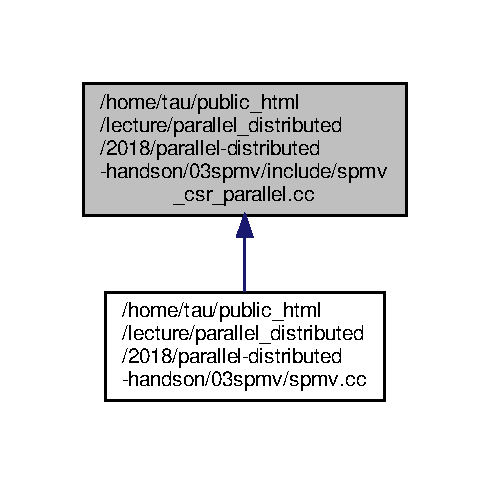
\includegraphics[width=235pt]{spmv__csr__parallel_8cc__dep__incl}
\end{center}
\end{figure}
\subsection*{Functions}
\begin{DoxyCompactItemize}
\item 
static int \hyperlink{spmv__csr__parallel_8cc_ae2c3871d937f3d196bfe193737ef2185}{spmv\+\_\+csr\+\_\+parallel} (\hyperlink{structsparse__t}{sparse\+\_\+t} A, \hyperlink{structvec__t}{vec\+\_\+t} vx, \hyperlink{structvec__t}{vec\+\_\+t} vy)
\begin{DoxyCompactList}\small\item\em y = A $\ast$ x for csr with parallel for \end{DoxyCompactList}\end{DoxyCompactItemize}


\subsection{Detailed Description}
y = A $\ast$ x for csr with parallel for 



\subsection{Function Documentation}
\mbox{\Hypertarget{spmv__csr__parallel_8cc_ae2c3871d937f3d196bfe193737ef2185}\label{spmv__csr__parallel_8cc_ae2c3871d937f3d196bfe193737ef2185}} 
\index{spmv\+\_\+csr\+\_\+parallel.\+cc@{spmv\+\_\+csr\+\_\+parallel.\+cc}!spmv\+\_\+csr\+\_\+parallel@{spmv\+\_\+csr\+\_\+parallel}}
\index{spmv\+\_\+csr\+\_\+parallel@{spmv\+\_\+csr\+\_\+parallel}!spmv\+\_\+csr\+\_\+parallel.\+cc@{spmv\+\_\+csr\+\_\+parallel.\+cc}}
\subsubsection{\texorpdfstring{spmv\+\_\+csr\+\_\+parallel()}{spmv\_csr\_parallel()}}
{\footnotesize\ttfamily static int spmv\+\_\+csr\+\_\+parallel (\begin{DoxyParamCaption}\item[{\hyperlink{structsparse__t}{sparse\+\_\+t}}]{A,  }\item[{\hyperlink{structvec__t}{vec\+\_\+t}}]{vx,  }\item[{\hyperlink{structvec__t}{vec\+\_\+t}}]{vy }\end{DoxyParamCaption})\hspace{0.3cm}{\ttfamily [static]}}



y = A $\ast$ x for csr with parallel for 


\begin{DoxyParams}{Parameters}
{\em (\+A)} & a sparse matrix \\
\hline
{\em (vx)} & a vector \\
\hline
{\em (vy)} & a vector \\
\hline
\end{DoxyParams}
\begin{DoxyReturn}{Returns}
1 if succeed, 0 if failed 
\end{DoxyReturn}

\hypertarget{spmv__csr__task_8cc}{}\section{/home/tau/public\+\_\+html/lecture/parallel\+\_\+distributed/2018/handson/tau/parallel-\/distributed-\/handson/03spmv/include/spmv\+\_\+csr\+\_\+task.cc File Reference}
\label{spmv__csr__task_8cc}\index{/home/tau/public\+\_\+html/lecture/parallel\+\_\+distributed/2018/handson/tau/parallel-\/distributed-\/handson/03spmv/include/spmv\+\_\+csr\+\_\+task.\+cc@{/home/tau/public\+\_\+html/lecture/parallel\+\_\+distributed/2018/handson/tau/parallel-\/distributed-\/handson/03spmv/include/spmv\+\_\+csr\+\_\+task.\+cc}}


y = A $\ast$ x for csr with tasks  


This graph shows which files directly or indirectly include this file\+:\nopagebreak
\begin{figure}[H]
\begin{center}
\leavevmode
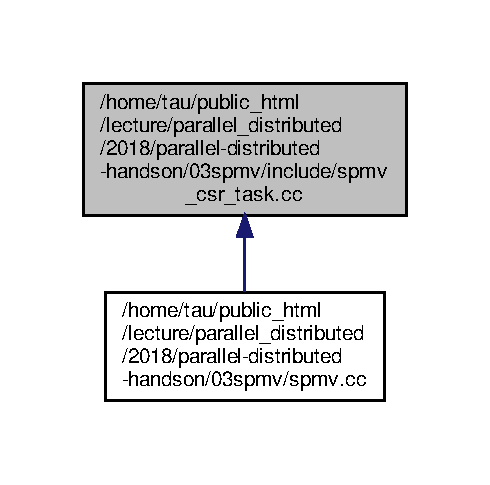
\includegraphics[width=262pt]{spmv__csr__task_8cc__dep__incl}
\end{center}
\end{figure}
\subsection*{Functions}
\begin{DoxyCompactItemize}
\item 
static int \hyperlink{spmv__csr__task_8cc_a3c9bfaecd18fdbead39a82c8b703efa8}{spmv\+\_\+csr\+\_\+task} (\hyperlink{structsparse__t}{sparse\+\_\+t} A, \hyperlink{structvec__t}{vec\+\_\+t} vx, \hyperlink{structvec__t}{vec\+\_\+t} vy)
\begin{DoxyCompactList}\small\item\em y = A $\ast$ x for csr with tasks \end{DoxyCompactList}\end{DoxyCompactItemize}


\subsection{Detailed Description}
y = A $\ast$ x for csr with tasks 



\subsection{Function Documentation}
\mbox{\Hypertarget{spmv__csr__task_8cc_a3c9bfaecd18fdbead39a82c8b703efa8}\label{spmv__csr__task_8cc_a3c9bfaecd18fdbead39a82c8b703efa8}} 
\index{spmv\+\_\+csr\+\_\+task.\+cc@{spmv\+\_\+csr\+\_\+task.\+cc}!spmv\+\_\+csr\+\_\+task@{spmv\+\_\+csr\+\_\+task}}
\index{spmv\+\_\+csr\+\_\+task@{spmv\+\_\+csr\+\_\+task}!spmv\+\_\+csr\+\_\+task.\+cc@{spmv\+\_\+csr\+\_\+task.\+cc}}
\subsubsection{\texorpdfstring{spmv\+\_\+csr\+\_\+task()}{spmv\_csr\_task()}}
{\footnotesize\ttfamily static int spmv\+\_\+csr\+\_\+task (\begin{DoxyParamCaption}\item[{\hyperlink{structsparse__t}{sparse\+\_\+t}}]{A,  }\item[{\hyperlink{structvec__t}{vec\+\_\+t}}]{vx,  }\item[{\hyperlink{structvec__t}{vec\+\_\+t}}]{vy }\end{DoxyParamCaption})\hspace{0.3cm}{\ttfamily [static]}}



y = A $\ast$ x for csr with tasks 


\begin{DoxyParams}{Parameters}
{\em (\+A)} & a sparse matrix \\
\hline
{\em (vx)} & a vector \\
\hline
{\em (vy)} & a vector \\
\hline
\end{DoxyParams}
\begin{DoxyReturn}{Returns}
1 if succeed, 0 if failed 
\end{DoxyReturn}

\hypertarget{spmv__csr__udr_8cc}{}\section{/home/tau/public\+\_\+html/lecture/parallel\+\_\+distributed/2018/handson/tau/parallel-\/distributed-\/handson/03spmv/include/spmv\+\_\+csr\+\_\+udr.cc File Reference}
\label{spmv__csr__udr_8cc}\index{/home/tau/public\+\_\+html/lecture/parallel\+\_\+distributed/2018/handson/tau/parallel-\/distributed-\/handson/03spmv/include/spmv\+\_\+csr\+\_\+udr.\+cc@{/home/tau/public\+\_\+html/lecture/parallel\+\_\+distributed/2018/handson/tau/parallel-\/distributed-\/handson/03spmv/include/spmv\+\_\+csr\+\_\+udr.\+cc}}


y = A $\ast$ x for csr with parallel for + user-\/defined functions  


This graph shows which files directly or indirectly include this file\+:\nopagebreak
\begin{figure}[H]
\begin{center}
\leavevmode
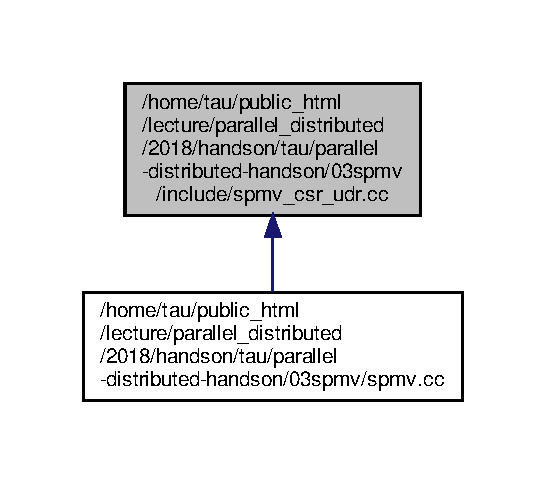
\includegraphics[width=262pt]{spmv__csr__udr_8cc__dep__incl}
\end{center}
\end{figure}
\subsection*{Functions}
\begin{DoxyCompactItemize}
\item 
static int \hyperlink{spmv__csr__udr_8cc_a9bee2a521f90ab82984586d212f437d3}{spmv\+\_\+csr\+\_\+udr} (\hyperlink{structsparse__t}{sparse\+\_\+t} A, \hyperlink{structvec__t}{vec\+\_\+t} vx, \hyperlink{structvec__t}{vec\+\_\+t} vy)
\begin{DoxyCompactList}\small\item\em y = A $\ast$ x for csr with parallel for + user-\/defined functions \end{DoxyCompactList}\end{DoxyCompactItemize}


\subsection{Detailed Description}
y = A $\ast$ x for csr with parallel for + user-\/defined functions 



\subsection{Function Documentation}
\mbox{\Hypertarget{spmv__csr__udr_8cc_a9bee2a521f90ab82984586d212f437d3}\label{spmv__csr__udr_8cc_a9bee2a521f90ab82984586d212f437d3}} 
\index{spmv\+\_\+csr\+\_\+udr.\+cc@{spmv\+\_\+csr\+\_\+udr.\+cc}!spmv\+\_\+csr\+\_\+udr@{spmv\+\_\+csr\+\_\+udr}}
\index{spmv\+\_\+csr\+\_\+udr@{spmv\+\_\+csr\+\_\+udr}!spmv\+\_\+csr\+\_\+udr.\+cc@{spmv\+\_\+csr\+\_\+udr.\+cc}}
\subsubsection{\texorpdfstring{spmv\+\_\+csr\+\_\+udr()}{spmv\_csr\_udr()}}
{\footnotesize\ttfamily static int spmv\+\_\+csr\+\_\+udr (\begin{DoxyParamCaption}\item[{\hyperlink{structsparse__t}{sparse\+\_\+t}}]{A,  }\item[{\hyperlink{structvec__t}{vec\+\_\+t}}]{vx,  }\item[{\hyperlink{structvec__t}{vec\+\_\+t}}]{vy }\end{DoxyParamCaption})\hspace{0.3cm}{\ttfamily [static]}}



y = A $\ast$ x for csr with parallel for + user-\/defined functions 


\begin{DoxyParams}{Parameters}
{\em (\+A)} & a sparse matrix \\
\hline
{\em (vx)} & a vector \\
\hline
{\em (vy)} & a vector \\
\hline
\end{DoxyParams}
\begin{DoxyReturn}{Returns}
1 if succeed, 0 if failed 
\end{DoxyReturn}

\hypertarget{vec__norm2__cuda_8cc}{}\section{/home/tau/public\+\_\+html/lecture/parallel\+\_\+distributed/2018/handson/tau/parallel-\/distributed-\/handson/03spmv/include/vec\+\_\+norm2\+\_\+cuda.cc File Reference}
\label{vec__norm2__cuda_8cc}\index{/home/tau/public\+\_\+html/lecture/parallel\+\_\+distributed/2018/handson/tau/parallel-\/distributed-\/handson/03spmv/include/vec\+\_\+norm2\+\_\+cuda.\+cc@{/home/tau/public\+\_\+html/lecture/parallel\+\_\+distributed/2018/handson/tau/parallel-\/distributed-\/handson/03spmv/include/vec\+\_\+norm2\+\_\+cuda.\+cc}}


the device procedure to do vec\+\_\+norm2 on the device  


\subsection*{Functions}
\begin{DoxyCompactItemize}
\item 
\+\_\+\+\_\+global\+\_\+\+\_\+ void \hyperlink{vec__norm2__cuda_8cc_afe19da671b9e7b759c966363ebff039c}{vec\+\_\+norm2\+\_\+dev} (\hyperlink{structvec__t}{vec\+\_\+t} v, \hyperlink{spmv_8cc_a11d147c64891830c9e79b3315b1b2e21}{real} $\ast$s)
\begin{DoxyCompactList}\small\item\em the device procedure to do vec\+\_\+norm2 on the device \end{DoxyCompactList}\item 
static \hyperlink{spmv_8cc_a11d147c64891830c9e79b3315b1b2e21}{real} \hyperlink{vec__norm2__cuda_8cc_a7dd3cfc8a09a071082c08d902a4ee7bc}{vec\+\_\+norm2\+\_\+cuda} (\hyperlink{structvec__t}{vec\+\_\+t} v)
\begin{DoxyCompactList}\small\item\em square norm of a vector in parallel with cuda \end{DoxyCompactList}\end{DoxyCompactItemize}


\subsection{Detailed Description}
the device procedure to do vec\+\_\+norm2 on the device 



\subsection{Function Documentation}
\mbox{\Hypertarget{vec__norm2__cuda_8cc_a7dd3cfc8a09a071082c08d902a4ee7bc}\label{vec__norm2__cuda_8cc_a7dd3cfc8a09a071082c08d902a4ee7bc}} 
\index{vec\+\_\+norm2\+\_\+cuda.\+cc@{vec\+\_\+norm2\+\_\+cuda.\+cc}!vec\+\_\+norm2\+\_\+cuda@{vec\+\_\+norm2\+\_\+cuda}}
\index{vec\+\_\+norm2\+\_\+cuda@{vec\+\_\+norm2\+\_\+cuda}!vec\+\_\+norm2\+\_\+cuda.\+cc@{vec\+\_\+norm2\+\_\+cuda.\+cc}}
\subsubsection{\texorpdfstring{vec\+\_\+norm2\+\_\+cuda()}{vec\_norm2\_cuda()}}
{\footnotesize\ttfamily static \hyperlink{spmv_8cc_a11d147c64891830c9e79b3315b1b2e21}{real} vec\+\_\+norm2\+\_\+cuda (\begin{DoxyParamCaption}\item[{\hyperlink{structvec__t}{vec\+\_\+t}}]{v }\end{DoxyParamCaption})\hspace{0.3cm}{\ttfamily [static]}}



square norm of a vector in parallel with cuda 


\begin{DoxyParams}{Parameters}
{\em (v)} & a vector \\
\hline
\end{DoxyParams}
\begin{DoxyReturn}{Returns}
the square norm of v (v\mbox{[}0\mbox{]}$^\wedge$2 + ... + v\mbox{[}n-\/1\mbox{]}$^\wedge$2) 
\end{DoxyReturn}
\mbox{\Hypertarget{vec__norm2__cuda_8cc_afe19da671b9e7b759c966363ebff039c}\label{vec__norm2__cuda_8cc_afe19da671b9e7b759c966363ebff039c}} 
\index{vec\+\_\+norm2\+\_\+cuda.\+cc@{vec\+\_\+norm2\+\_\+cuda.\+cc}!vec\+\_\+norm2\+\_\+dev@{vec\+\_\+norm2\+\_\+dev}}
\index{vec\+\_\+norm2\+\_\+dev@{vec\+\_\+norm2\+\_\+dev}!vec\+\_\+norm2\+\_\+cuda.\+cc@{vec\+\_\+norm2\+\_\+cuda.\+cc}}
\subsubsection{\texorpdfstring{vec\+\_\+norm2\+\_\+dev()}{vec\_norm2\_dev()}}
{\footnotesize\ttfamily \+\_\+\+\_\+global\+\_\+\+\_\+ void vec\+\_\+norm2\+\_\+dev (\begin{DoxyParamCaption}\item[{\hyperlink{structvec__t}{vec\+\_\+t}}]{v,  }\item[{\hyperlink{spmv_8cc_a11d147c64891830c9e79b3315b1b2e21}{real} $\ast$}]{s }\end{DoxyParamCaption})}



the device procedure to do vec\+\_\+norm2 on the device 


\begin{DoxyParams}{Parameters}
{\em (v)} & a vector \\
\hline
{\em (s)} & a pointer to a device memory to put the result into\\
\hline
\end{DoxyParams}
assume v.\+elems\+\_\+dev already set and s a proper pointer to a device memory 
\hypertarget{vec__norm2__parallel_8cc}{}\section{/home/tau/public\+\_\+html/lecture/parallel\+\_\+distributed/2018/parallel-\/distributed-\/handson/03spmv/include/vec\+\_\+norm2\+\_\+parallel.cc File Reference}
\label{vec__norm2__parallel_8cc}\index{/home/tau/public\+\_\+html/lecture/parallel\+\_\+distributed/2018/parallel-\/distributed-\/handson/03spmv/include/vec\+\_\+norm2\+\_\+parallel.\+cc@{/home/tau/public\+\_\+html/lecture/parallel\+\_\+distributed/2018/parallel-\/distributed-\/handson/03spmv/include/vec\+\_\+norm2\+\_\+parallel.\+cc}}


square norm of a vector in serial  


This graph shows which files directly or indirectly include this file\+:\nopagebreak
\begin{figure}[H]
\begin{center}
\leavevmode
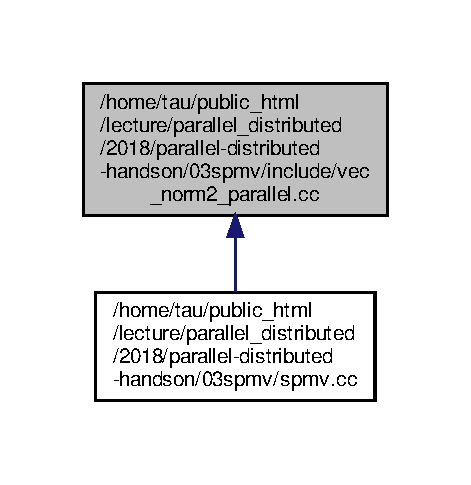
\includegraphics[width=226pt]{vec__norm2__parallel_8cc__dep__incl}
\end{center}
\end{figure}
\subsection*{Functions}
\begin{DoxyCompactItemize}
\item 
static \hyperlink{spmv_8cc_a11d147c64891830c9e79b3315b1b2e21}{real} \hyperlink{vec__norm2__parallel_8cc_a93ea4592e149a2ef18aea41dce0f1cbb}{vec\+\_\+norm2\+\_\+parallel} (\hyperlink{structvec__t}{vec\+\_\+t} v)
\begin{DoxyCompactList}\small\item\em square norm of a vector in serial \end{DoxyCompactList}\end{DoxyCompactItemize}


\subsection{Detailed Description}
square norm of a vector in serial 



\subsection{Function Documentation}
\mbox{\Hypertarget{vec__norm2__parallel_8cc_a93ea4592e149a2ef18aea41dce0f1cbb}\label{vec__norm2__parallel_8cc_a93ea4592e149a2ef18aea41dce0f1cbb}} 
\index{vec\+\_\+norm2\+\_\+parallel.\+cc@{vec\+\_\+norm2\+\_\+parallel.\+cc}!vec\+\_\+norm2\+\_\+parallel@{vec\+\_\+norm2\+\_\+parallel}}
\index{vec\+\_\+norm2\+\_\+parallel@{vec\+\_\+norm2\+\_\+parallel}!vec\+\_\+norm2\+\_\+parallel.\+cc@{vec\+\_\+norm2\+\_\+parallel.\+cc}}
\subsubsection{\texorpdfstring{vec\+\_\+norm2\+\_\+parallel()}{vec\_norm2\_parallel()}}
{\footnotesize\ttfamily static \hyperlink{spmv_8cc_a11d147c64891830c9e79b3315b1b2e21}{real} vec\+\_\+norm2\+\_\+parallel (\begin{DoxyParamCaption}\item[{\hyperlink{structvec__t}{vec\+\_\+t}}]{v }\end{DoxyParamCaption})\hspace{0.3cm}{\ttfamily [static]}}



square norm of a vector in serial 


\begin{DoxyParams}{Parameters}
{\em (v)} & a vector \\
\hline
\end{DoxyParams}
\begin{DoxyReturn}{Returns}
the square norm of v (v\mbox{[}0\mbox{]}$^\wedge$2 + ... + v\mbox{[}n-\/1\mbox{]}$^\wedge$2) 
\end{DoxyReturn}

\hypertarget{vec__norm2__task_8cc}{}\section{/home/tau/public\+\_\+html/lecture/parallel\+\_\+distributed/2018/parallel-\/distributed-\/handson/03spmv/include/vec\+\_\+norm2\+\_\+task.cc File Reference}
\label{vec__norm2__task_8cc}\index{/home/tau/public\+\_\+html/lecture/parallel\+\_\+distributed/2018/parallel-\/distributed-\/handson/03spmv/include/vec\+\_\+norm2\+\_\+task.\+cc@{/home/tau/public\+\_\+html/lecture/parallel\+\_\+distributed/2018/parallel-\/distributed-\/handson/03spmv/include/vec\+\_\+norm2\+\_\+task.\+cc}}


square norm of a vector in serial  


This graph shows which files directly or indirectly include this file\+:\nopagebreak
\begin{figure}[H]
\begin{center}
\leavevmode
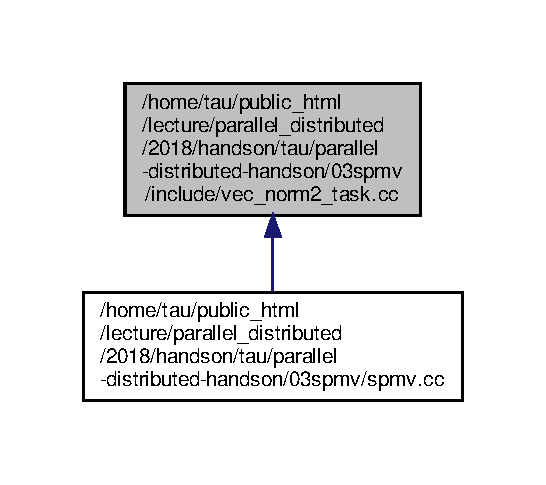
\includegraphics[width=226pt]{vec__norm2__task_8cc__dep__incl}
\end{center}
\end{figure}
\subsection*{Functions}
\begin{DoxyCompactItemize}
\item 
static \hyperlink{spmv_8cc_a11d147c64891830c9e79b3315b1b2e21}{real} \hyperlink{vec__norm2__task_8cc_a66ae15550f3329b3c276dead7d8b7ffc}{vec\+\_\+norm2\+\_\+task} (\hyperlink{structvec__t}{vec\+\_\+t} v)
\begin{DoxyCompactList}\small\item\em square norm of a vector in serial \end{DoxyCompactList}\end{DoxyCompactItemize}


\subsection{Detailed Description}
square norm of a vector in serial 



\subsection{Function Documentation}
\mbox{\Hypertarget{vec__norm2__task_8cc_a66ae15550f3329b3c276dead7d8b7ffc}\label{vec__norm2__task_8cc_a66ae15550f3329b3c276dead7d8b7ffc}} 
\index{vec\+\_\+norm2\+\_\+task.\+cc@{vec\+\_\+norm2\+\_\+task.\+cc}!vec\+\_\+norm2\+\_\+task@{vec\+\_\+norm2\+\_\+task}}
\index{vec\+\_\+norm2\+\_\+task@{vec\+\_\+norm2\+\_\+task}!vec\+\_\+norm2\+\_\+task.\+cc@{vec\+\_\+norm2\+\_\+task.\+cc}}
\subsubsection{\texorpdfstring{vec\+\_\+norm2\+\_\+task()}{vec\_norm2\_task()}}
{\footnotesize\ttfamily static \hyperlink{spmv_8cc_a11d147c64891830c9e79b3315b1b2e21}{real} vec\+\_\+norm2\+\_\+task (\begin{DoxyParamCaption}\item[{\hyperlink{structvec__t}{vec\+\_\+t}}]{v }\end{DoxyParamCaption})\hspace{0.3cm}{\ttfamily [static]}}



square norm of a vector in serial 


\begin{DoxyParams}{Parameters}
{\em (v)} & a vector \\
\hline
\end{DoxyParams}
\begin{DoxyReturn}{Returns}
the square norm of v (v\mbox{[}0\mbox{]}$^\wedge$2 + ... + v\mbox{[}n-\/1\mbox{]}$^\wedge$2) 
\end{DoxyReturn}

\hypertarget{vec__norm2__udr_8cc}{}\section{/home/tau/public\+\_\+html/lecture/parallel\+\_\+distributed/2018/parallel-\/distributed-\/handson/03spmv/include/vec\+\_\+norm2\+\_\+udr.cc File Reference}
\label{vec__norm2__udr_8cc}\index{/home/tau/public\+\_\+html/lecture/parallel\+\_\+distributed/2018/parallel-\/distributed-\/handson/03spmv/include/vec\+\_\+norm2\+\_\+udr.\+cc@{/home/tau/public\+\_\+html/lecture/parallel\+\_\+distributed/2018/parallel-\/distributed-\/handson/03spmv/include/vec\+\_\+norm2\+\_\+udr.\+cc}}


square norm of a vector in parallel using user-\/defined reduction  


This graph shows which files directly or indirectly include this file\+:\nopagebreak
\begin{figure}[H]
\begin{center}
\leavevmode
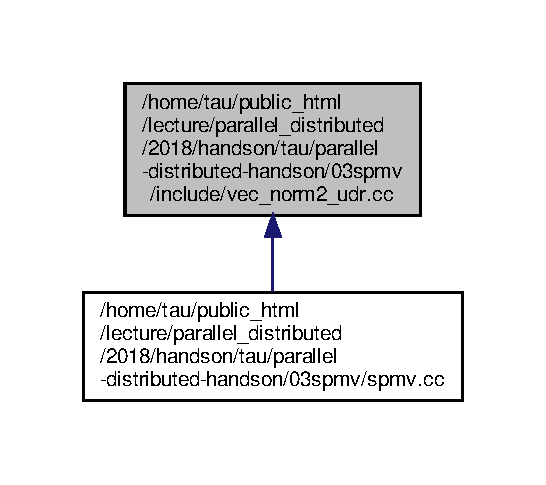
\includegraphics[width=226pt]{vec__norm2__udr_8cc__dep__incl}
\end{center}
\end{figure}
\subsection*{Functions}
\begin{DoxyCompactItemize}
\item 
static \hyperlink{spmv_8cc_a11d147c64891830c9e79b3315b1b2e21}{real} \hyperlink{vec__norm2__udr_8cc_a7559fa49346e732e2002df9c70512d6a}{vec\+\_\+norm2\+\_\+udr} (\hyperlink{structvec__t}{vec\+\_\+t} v)
\begin{DoxyCompactList}\small\item\em square norm of a vector in parallel using user-\/defined reduction \end{DoxyCompactList}\end{DoxyCompactItemize}


\subsection{Detailed Description}
square norm of a vector in parallel using user-\/defined reduction 



\subsection{Function Documentation}
\mbox{\Hypertarget{vec__norm2__udr_8cc_a7559fa49346e732e2002df9c70512d6a}\label{vec__norm2__udr_8cc_a7559fa49346e732e2002df9c70512d6a}} 
\index{vec\+\_\+norm2\+\_\+udr.\+cc@{vec\+\_\+norm2\+\_\+udr.\+cc}!vec\+\_\+norm2\+\_\+udr@{vec\+\_\+norm2\+\_\+udr}}
\index{vec\+\_\+norm2\+\_\+udr@{vec\+\_\+norm2\+\_\+udr}!vec\+\_\+norm2\+\_\+udr.\+cc@{vec\+\_\+norm2\+\_\+udr.\+cc}}
\subsubsection{\texorpdfstring{vec\+\_\+norm2\+\_\+udr()}{vec\_norm2\_udr()}}
{\footnotesize\ttfamily static \hyperlink{spmv_8cc_a11d147c64891830c9e79b3315b1b2e21}{real} vec\+\_\+norm2\+\_\+udr (\begin{DoxyParamCaption}\item[{\hyperlink{structvec__t}{vec\+\_\+t}}]{v }\end{DoxyParamCaption})\hspace{0.3cm}{\ttfamily [static]}}



square norm of a vector in parallel using user-\/defined reduction 


\begin{DoxyParams}{Parameters}
{\em (v)} & a vector \\
\hline
\end{DoxyParams}
\begin{DoxyReturn}{Returns}
the square norm of v (v\mbox{[}0\mbox{]}$^\wedge$2 + ... + v\mbox{[}n-\/1\mbox{]}$^\wedge$2) 
\end{DoxyReturn}

\hypertarget{vec__to__dev_8cc}{}\section{/home/tau/public\+\_\+html/lecture/parallel\+\_\+distributed/2018/parallel-\/distributed-\/handson/03spmv/include/vec\+\_\+to\+\_\+dev.cc File Reference}
\label{vec__to__dev_8cc}\index{/home/tau/public\+\_\+html/lecture/parallel\+\_\+distributed/2018/parallel-\/distributed-\/handson/03spmv/include/vec\+\_\+to\+\_\+dev.\+cc@{/home/tau/public\+\_\+html/lecture/parallel\+\_\+distributed/2018/parallel-\/distributed-\/handson/03spmv/include/vec\+\_\+to\+\_\+dev.\+cc}}


make a deivce copy of a vector.  


\subsection*{Functions}
\begin{DoxyCompactItemize}
\item 
static int \hyperlink{vec__to__dev_8cc_a526773beced925dd5db091a60d74fdcf}{vec\+\_\+to\+\_\+dev} (\hyperlink{structvec__t}{vec\+\_\+t} \&v)
\begin{DoxyCompactList}\small\item\em make a deivce copy of a vector. \end{DoxyCompactList}\end{DoxyCompactItemize}


\subsection{Detailed Description}
make a deivce copy of a vector. 



\subsection{Function Documentation}
\mbox{\Hypertarget{vec__to__dev_8cc_a526773beced925dd5db091a60d74fdcf}\label{vec__to__dev_8cc_a526773beced925dd5db091a60d74fdcf}} 
\index{vec\+\_\+to\+\_\+dev.\+cc@{vec\+\_\+to\+\_\+dev.\+cc}!vec\+\_\+to\+\_\+dev@{vec\+\_\+to\+\_\+dev}}
\index{vec\+\_\+to\+\_\+dev@{vec\+\_\+to\+\_\+dev}!vec\+\_\+to\+\_\+dev.\+cc@{vec\+\_\+to\+\_\+dev.\+cc}}
\subsubsection{\texorpdfstring{vec\+\_\+to\+\_\+dev()}{vec\_to\_dev()}}
{\footnotesize\ttfamily static int vec\+\_\+to\+\_\+dev (\begin{DoxyParamCaption}\item[{\hyperlink{structvec__t}{vec\+\_\+t} \&}]{v }\end{DoxyParamCaption})\hspace{0.3cm}{\ttfamily [static]}}



make a deivce copy of a vector. 


\begin{DoxyParams}{Parameters}
{\em (v)} & the reference to a matrix whose elems\+\_\+dev has not been set (i.\+e., = N\+U\+LL) \\
\hline
\end{DoxyParams}
\begin{DoxyReturn}{Returns}
1 if succeed. 0 if failed. 
\end{DoxyReturn}
\begin{DoxySeeAlso}{See also}
sparse\+\_\+to\+\_\+dev 
\end{DoxySeeAlso}

%--- End generated contents ---

% Index
\backmatter
\newpage
\phantomsection
\clearemptydoublepage
\addcontentsline{toc}{chapter}{Index}
\printindex

\end{document}
